\documentclass[fontsize = 12pt,						%Schriftgröße
paper = a4,								%Papierformat
headings = small,					%Größe der Überschriften
open=right,								%Abschnitte beginnen rechts
cleardoublepage = empty,		%leere Seiten ohne Kopfzeile
BCOR = 10mm,								%Binde Korrektur
captions = tableheading,		%Tabellen mit Überschriften
bibliography = totoc,			%Literatur- ins Inhaltsverzeichnis
listof = totoc,						%Verzeichnisse ins Inhaltsverzeichnis
twoside = false]						%doppelseitiges Layout
{scrbook}										%Dokumentklasse

% headsepline Auslassen von Kopfzeilen bei Kapiteln und titlepage das Auslassen von einer Titelseitennummerierung
%\usepackage[ngerman]{babel} % Für die deutsche Sprache
%\usepackage{ngerman}
\usepackage{eurosym} % Eurozeichen
%\usepackage[utf8]{inputenc} % Für deutsche Umlaute
\usepackage{graphicx} % Für die Einbringung von Graphiken
\usepackage{subcaption} % Für das Darstellen von Graphiken nebeneinander
\usepackage{multirow} % Für Tabellen, 1 Zeile auf 2 Zeilen
\usepackage{tocvsec2} % Für das Herausnehmen von Untersektionen aus dem Inhaltsverzeichnis (settocdepth{section})
\usepackage{setspace} % Für den Zeilenabstand
\usepackage{scrhack} %um den error \float@listhead detected!(scrartcl)
\usepackage{booktabs} % Für unterschiedlich Breite senkrechte Tabellenlinien (vertikale Linien können als unnötig angesehen werden)
\usepackage{pdfpages} % Um pdfs zu inkludieren
\usepackage{float} % Platziert Abbildungen an exakt dem Platz   [H]
\usepackage{pstricks}
 %\usepackage[style=numeric,backend=biber,giveninits=true,doi=false,isbn=false,url=false]{biblatex} %Für die Bibliography
 \usepackage[style=numeric,backend=biber,doi=false,isbn=false]{biblatex} %Für die Bibliography
 \DefineBibliographyStrings{american}{phdthesis = {PhD dissertation}}
 \bibliography{bib} %Ort der Bibliography
 \usepackage{csquotes} %Für zitieren mit biblatex notwendig
 
\usepackage{amsmath, amsthm, amssymb, amsfonts} % Für das Darstellen von Formeln

\usepackage{pifont} % xmark und checkmark
\newcommand{\cmark}{\ding{51}}%
\newcommand{\xmark}{\ding{55}}%

\numberwithin{equation}{section}   % Nummerierung der Formeln abschnittsweise
  
\usepackage{gensymb} % Für das darstellen von degree
  
\usepackage{chngcntr} %Für kapitelweise Nummerierung der Abbildungen
  \counterwithout{figure}{section}
  \counterwithout{figure}{subsection}
  %\counterwithin{figure}{chapter}
  
\usepackage{xcolor} %Für ein dunkleres blau zum besseren Drucken
  \definecolor{ultramarine}{RGB}{0,32,96}

\usepackage[printonlyused, nohyperlinks]{acronym} %Für ein Abkürzungsverzeichnis, nur benutzte Abkürzungen werden 	  aufgeführt, keine hyperlinks weil diese sonst gefärbt sein würden
  \renewcommand*{\acsfont}[1]{{\color{black}\text{#1}}} % Setzt die Farbe der Abkürzungen im Text auf schwarz

\usepackage{tikz} %Für Ablaufdiagramm und andere Zeichnungen
\usetikzlibrary{matrix,shapes,arrows,positioning,chains}
\usetikzlibrary{calc,patterns,angles,quotes} % Um Grad einzuzeichnen
\usetikzlibrary{trees} % Für entscheidungsbäume
\tikzstyle{decision} = [diamond, draw, text width=4.5em,node distance=3.5cm, text badly centered,inner sep=0pt] %Definiert den Entscheidungsblock 
\tikzstyle{block} = [rectangle, draw, text centered, rounded corners,   ] %minimum height=4em,text width=20em  %Definiert den Anweisungsblock
\tikzstyle{line} = [draw, -latex'] %Definiert die Verbindungslinie

\usepackage{forest} % u.a. Für das Darstellen von horizontalen Entscheidungsbäumen 
\usetikzlibrary{positioning}
 \usetikzlibrary{arrows,decorations.pathmorphing,backgrounds,fit,positioning,shapes.symbols,chains} % Für Systemdiagramme

\usepackage{hyperref} % Für Querverweise im Inhaltsverzeichnis auf Kapitel (Auch Adobe Reader Infos möglich)
  \hypersetup{hidelinks,% Keine Box und keine Farbe für Querverweise
	      colorlinks   = true, %gefärbte Links anstatt Boxen 
	      allcolors=black,   %Jede Farbe auf blau
	      linktocpage % Seitenzahlen werden gefärbt, nicht die Buchstaben
  }
  \texorpdfstring{}{} %Formeln in hyperref angezeigt werden können.
 
\usepackage{pythonhighlight} % Darstellen von Python Programmierung
 
\usepackage{listings} % Für das Einfügen von Quelltext 
  \renewcommand{\lstlistingname}{Code} % Für das Ändern der Quellcode Unterschriften
  \renewcommand{\lstlistlistingname}{List Code} % Für das Ändern der Quellcodeverzeichnis Überschrift
  \lstset{ % Einstellungen für listings
    language=python, % Programmiersprache
    numbers=left, % Zeilennummern links anzeigen
      numbersep=-15pt,   % Abstand zwischen Nummer und Code
    basicstyle=\footnotesize, % Größe der Quellcode Buchstaben
    captionpos=b, % Position einer Beschriftung
       xleftmargin={-0.2cm}, % Abstand zum linken Rand um Zeilennummern an Text auszurichten
%    xleftmargin=\textwidth, xrightmargin=\textwidth
  }

\usepackage{scrpage2}
\usepackage{scrhack}
\pagestyle{scrheadings}
\automark[section]{chapter}
\addtokomafont{pageheadfoot}{\normalfont\sffamily}
\addtokomafont{pagenumber}{\normalfont\sffamily\bfseries}
\setheadsepline{0.4pt}
\clearscrheadfoot
%\cehead[]{\leftmark}
%\cohead[]{\rightmark}
\ohead[]{\pagemark}
\ofoot[\pagemark]{}
\ihead[]{\leftmark}
\ihead[]{\rightmark}
\usepackage{lmodern}
\usepackage[T1]{fontenc}
\usepackage{graphicx}

\usepackage{afterpage} % Für eine leere Seite
\newcommand\blankpage{%
	\null
	\thispagestyle{empty}%
	\addtocounter{page}{-1}%
	\newpage}

\usepackage[Sonny]{fncychap}		%Sonny/Lenny/Glenn/Conny/Rejne/Bjarne
\ChTitleVar{\LARGE\bfseries}
\ChNameVar{\large\bfseries}
\begin{document}

   \renewcommand*{\chapterpagestyle}{empty}
  
   \frontmatter

  \clearpage
   %-----------------------------------------------------------------------------%
%                                                                             %
%    T I T E L S E I T E                                                      %
%                                                                             %
%-----------------------------------------------------------------------------%
%
\thispagestyle{empty}
\hypersetup{pageanchor=false}


%
\begin{center}
\vspace*{5cm} 
\Large
\textsf{Final Project}
\vspace*{1cm} 

\textsf{Development of a software architecture for virtual sensors in an autonomous small vessel for inland waterways.\footnote{Revisited version without formal part and with reduced number of external figures. }}\\

\normalsize
\vspace*{1cm} 
August 05, 2021\\ \vspace*{0.5cm} 
Jonas Mahler

\end{center}



  %\afterpage{\blankpage}
   \clearpage
   \makeatletter\@openrightfalse
   \chapter*{Abstract}
This project takes place in the context of the research project \ac{ELLA} that is funded by the German Federal Ministry of Transport and Digital Infrastructure. In this project, automated  manoeuvring of inland navigation vessels in confined spaces such as flood gates and harbours is investigated with a simulated virtual environment and a subsequent verification of the simulation results with a model scaled small vessel of an actual inland navigation vessel. The aim of this thesis is to develop a software architecture that allows for the integration of virtual sensors in the navigation subsystem of a guidance, navigation and control system of a small vessel in the inland navigation sector. In addition to the integration of virtual sensors, the architecture should be easily extendable towards the utilization of real sensors.\\
% The environment contains a scaled height map of the project specific location and is modelled according to the geographic characterisations of the real environment
 
The system is realized within the framework supplied by ROS2 in conjunction with Node.js and a virtual environment that is set up in a game engine provided by Unity3d. As a first step a virtual environment is set up in Unity3d. A small vessel that is contained in the virtual environment is equipped with virtual sensors such as a \ac{LIDAR} and an \ac{IMU}. The sensors publish its data with customized messages via Node.js that serves as a transition, to ROS2. In ROS2 the distinction between the three subsystems of the \ac{GNC} system is made and the sensor data is preprocessed by the navigation subsystem if necessary.\\

The results show that the chosen frameworks and algorithms allow for virtual data generation and subsequent data processing and visualization. It is demonstrated that the designed software architecture allows for the modular integration of  both virtual elements and algorithms. Ways to extend the design are outlined as well as improvements related to the performance of the implemented modules.
\chapter*{Kurzfassung}

Diese Projektarbeit findet im Rahmen des Forschungsvorhaben \ac{ELLA} statt, das vom Bundesministerium für Verkehr und digitale Infrastruktur gefördert wird. In diesem Projekt wird das automatisierte Manövrieren von Binnenschiffen in engen Räumen wie Schleusen und Häfen mit einer simulierten virtuellen Umgebung und einer anschließenden Verifikation der Simulationsergebnisse mit einem maßstabsgetreuen Kleinfahrzeug eines realen Binnenschiffs untersucht. Ziel dieser Arbeit ist es, eine Softwarearchitektur zu entwickeln, welche die Integration virtueller Sensoren in das Navigationssubsystem eines Führungs-, Navigations- und Steuerungssystems eines Binnenschiffs ermöglicht. Neben der Integration virtueller Sensoren soll die Architektur auch für die Nutzung realer Sensoren erweiterbar sein. Realisiert wird das System innerhalb des von ROS2 bereitgestellten Frameworks in Verbindung mit Node.js und einer virtuellen Umgebung, die in einer von Unity3d Game-Engine umgesetzt wird. \\


In einem ersten Schritt wird eine virtuelle Umgebung in Unity3d erstellt. Ein Kleinfahrzeug, das sich in der virtuellen Umgebung befindet, ist mit virtuellen Sensoren wie einem \ac{LIDAR} und einer \ac{IMU} ausgestattet. Die Sensoren veröffentlichen ihre Daten mit Nachrichten über Node.js, das als Übergang dient, an ROS2. In ROS2 wird die Unterscheidung zwischen den drei Subsystemen des \ac{GNC}-Systems vorgenommen und die Sensordaten werden bei Bedarf durch das Navigationssubsystem vorverarbeitet.\\

Die Ergebnisse zeigen, dass die gewählten Frameworks und Algorithmen eine virtuelle Datengenerierung und anschließende Datenverarbeitung und Visualisierung ermöglichen. Es wird gezeigt, dass die entworfene Software-Architektur eine modulare Integration sowohl von virtuellen Elementen als auch von Algorithmen ermöglicht. Möglichkeiten zur Erweiterung des Designs werden ebenso aufgezeigt wie Verbesserungen in Bezug auf die Leistung der implementierten Module.


   

  \@openrighttrue\makeatother 
   \tableofcontents
  
   \clearpage
   %\addchap*{Abbreviations} %Asterix (*) lässt Kapitel ohne Nummern, ohne Inhaltsverzeichniseintrag
  \begin{acronym}[SOCA-CFAR] % Abkürzungsverzeichnis, längste Abkürzung in []
  \renewcommand{\\}{}
  \begin{spacing}{0.7} % ändert den Zeilenabstand von default auf einen anderen Wert
  \acro{USV}{Unmanned Surface Vehicle}
  \acroplural{USV}{Unmanned Surface Vehicles} % (acp{})
  \acro{GNC}{Guidance, Navigation and Control}
  \acro{LIDAR}{Light Detection and Ranging}
  \acro{GNSS}{Global Navigation Satellite System}
  \acro{IMU}{Intertial Measurement Unit}
  \acro{MOOS-IvP}{Mission Oriented Operating Suite-Interval Programming}
  \acro{PID}{Proportional Integral Derivative}
  \acro{PLC}{Programmable Logic Control}
  \acro{RADAR}{Radio Detection and Ranging}
  \acro{LASER}{Light Amplification by Stimulated Emission of Radiation}
  \acro{CFT}{Clustering Feature Tree}
  \acro{CF}{Clustering Feature}
  \acro{BIRCH}{Balanced Iterative Reducing and Clustering using Hierarchies}
  \acro{MTD}{Moving Target Detection}
  \acro{SNR}{Signal Noise Ratio}
  \acro{CFAR}{Constant False Alarm Rate}
  \acro{OS-CFAR}{Ordered Statistics Constant False Alarm Rate}
  \acro{PDF}{Probability Density Function}
  \acroplural{PDF}{Probability Density Functions}
  \acro{CUT}{Cell Under Test}
  \acro{DBSCAN}{Density Based Spatial Clustering of Applications with Noise}
  \acro{SONAR}{Sound Navigation and Ranging}
  \acro{WLAN}{Wireless Local Area Network}
  \acro{SDK}{Software Development Kit}
  \acro{CARACAS}{Control Architecture for Robotic Agent Command and Sensing}
  \acro{ROS}{Robot Operating System}
  \acro{CAN}{Controller Area Network}
  \acro{GPU}{Graphics Processing Unit}
  \acro{API}{Application Programming Interface}
  \acro{HMI}{Human Machine Interface}
  \acro{FOV}{Field of View}
  \acro{LAN}{Local Area Network}
  \acro{LAESSI}{Guiding and Assistance Systems to Improve Safety of Navigation on Inland Waterways}
  \acro{RTK}{Real Time Kinematics}
  \acro{CPU}{Central Processing Unit}
  \acro{MASS}{Maritime Autonomous Surface Ships}
  \acro{VDE}{Association for Electrical, Electronic and Information Technologies}
  \acro{ISO}{International Organization for Standardization}
  \acro{IMO}{International Maritime Organization}
  \acro{IEEE}{Institute of Electrical and Electronics Engineers}
  \acro{IEC}{International Electrotechnical Commission}
  \acro{DDS}{Data Distribution Service}
  \acro{RTT}{Round Trip Time}
  \acro{TCP}{Transmission Control Protocol}
  \acro{JSON}{JavaScript Object Notation}
  \acro{ELLA}{Model Scale Development Platform for Maneuver Automation/ Entwicklungsplattform im Modellmaßstab für Manöver-Automatisierung}
  \acro{ROS2}{Roboter Operating System 2}
  \acro{TIN}{Triangulated Irregular Network}
  \acro{DEM}{Digital Elevation Model}
  \acro{SOCA-CFAR}{Smallest of Cell Averaging-CFAR}
  \end{spacing}
  \end{acronym}
 % Auflistung der Abkürzungen
  

  \mainmatter % den Hauptteil beginnen
   \clearpage

   \pagestyle{scrheadings}  % Kopfzeilen
   \thispagestyle{scrheadings}  % Kopfzeilen

  
\chapter{Introduction}\label{Introduction}
  \section{Motivation}

With the increasing relevance of climate change new concepts for mobility are required. A change in mobility demands not only decreasing carbon emissions but also increasing flexibility in order to remain competitive in an international context. With the strategic plan "Transport 2050" the European Commission sets targets to increase mobility in the European Union and to reduce emissions at the same time. Among these targets is the requirement to shift freight transport from road to rail and water. This is to be implemented by 2050 for 30\% of freight transports over 300km \cite{Transport2050}. Within the European Union, Germany proposed a national master plan specifically for the future of inland navigation in which the importance of inland navigation for a sustainable future is further highlighted. One important aspect is to increase the transport of goods by inland navigation to reach 12,3\% of total transported goods until 2030 \cite{MasterplanBinnen}. These requirements can be set against a background of increasing congestion on the roads and at the same time overcapacity of transport by water. In the context of these changes, waterborne transport, and in particular inland navigation, must prove to be competitive both economically and in terms of sustainability \cite{Christa2020}.\\

The automatisation of inland navigation vessels up to the possibility of an unmanned operated or autonomous vessels can play a vital role to full fill this requirements. There are expected to be huge advantages in operating \acp{USV} in comparison to traditional operated vehicles. With the automatisation of the vehicles comes an reduction of crew members to control a vehicle and hence the operational cost are reduced. Furthermore the reliability and flexibility in harsh or otherwise sophisticated environments increases. Particularly in shallow waters this flexibility allows an adaption of the \ac{USV} towards the requirements of this environment \cite{Liu2016}.\\

The technological innovation efforts of the inland navigation sector comprised mainly the development of low-emission engines \cite{Christa2020}. However, research into the field of \acp{USV} has been pursued over the past two decades. Even so, most current research is conducted on relatively small vehicles with limited capabilities regarding autonomy, endurance, payload and power outputs and experimental research remains an important topic for the future \cite{Liu2016}. \\

Therefore, designing a vessel specifically for autonomous operation to evaluate technologies for the next generation of inland navigation vessels is an important step towards further innovations in this sector. More specifically, the vessel should be able to sense its environment and operational state to enable situational awareness and autonomous decision making, possibly with the application of machine learning. Simulated environments provide an opportunity to facilitate the process of sensor data generation by means of virtual sensors. Therefore a software architecture that supports both real world and virtual appliance is of great importance in the design process of such a vessel.  


 \section{Previous work}\label{previous}
  
 Within the research project \ac{LAESSI}, a driver assistance system was designed and implemented on an inland navigation vessel with the focus on a bridge collision warning system and instruments to visualize the internal and external state of the vessel. To localize the vessels position, a land based corrected \ac{GNSS} signal was used together with electronic charts and further information transmitted from a land based station as for example temporarily restrictions caused by construction sides and the current water level. Internal sensors comprise a inertial measurement unit, a height sensor and turn indicator. The sensors data together with the \ac{GNSS} data are processed and checked for integrity as errors in the positing data directly influences the rudder commands in the chosen system architecture \cite{LAESSI}. The sensors in this research project however do not allow the vessel a land station independent representation of its environment and thus the vessel depends on an established connection to a land based station to function properly.\\
 
 A first step towards a higher degree of automatisation with the focus on reducing crew members to operate a vessel was laid by the KU Leuven with the vessel "Cogge". A design for an automated vessel is proposed with focus on the three key technological design aspects industrial relevance, vessel-environment interactions and the motions control of the vessel. The design is in accordance with an EU co financed vessel design project Watertruck+ \cite{watertruck}, in which standardised and modular small barges and push boats allow a high degree of flexibility especially in small waterways. The sensors of the "Cogge" comprising \ac{GNSS}, \ac{IMU}, \ac{LIDAR} and stereo image sensors. The software for the motion control is organized in a multilayered software design. To determine the route, waypoints are generated based on an open source map which then can be utilized by the middle level control. Software for the middle level control is provided by the \ac{MOOS-IvP} system \cite{MOOS}, a set of open source software modules specifically for the operation of autonomous marine vehicles. To reduce the error between the current and the desired speed and direction, a \ac{PID} controller compares the \ac{GNSS} and \ac{IMU} sensor values with given data of the \ac{MOOS-IvP}. The \ac{PID} controller connected with a downstream \ac{PLC} is implemented in the lower level control. Experiments conducted with this platform however has tended to focus on following generated waypoints with optimizing course deviations\cite{Peeters2020}. The integration of sensors beyond \ac{IMU} and \ac{GNSS} and the ability to manoeuvre in confined spaces as necessary in weir and lock systems remains open. Furthermore, the outlined design is lacking a \ac{RADAR} system to generate spatial data for objects further away than the range of the \ac{LIDAR}. That also leaves open the question how to merge the \ac{RADAR} and \ac{LIDAR} data at its transition.\\
 
 With increasing interest in autonomous driving especially in the field of automotive during the recent years, the research into automotive systems that integrates a wide variety of sensors is considerably more detailed compared to the inland navigation sector or more generally compared to water bound vehicles. A software-stack framework that is called "Autoware" provides an example of such a system designed to enable autonomous driving of vehicles. It is based on \ac{ROS}, an opensource middleware framework developed for robot applications and is open source itself. The required sensors that are used by the software can be purchased on the market and comprise a \ac{LIDAR}, a camera, \ac{GNSS}  with \ac{RTK} in the proposed system. On the software side, the tasks of algorithms are divided into the classes scene recognition, path planning and vehicle control. For each of these classes a set of algorithms is proposed. The software is run on an Nvidia \ac{GPU}, which allows for example for a faster object detection compared to \ac{CPU} based computation \cite{Autoware}. In a subsequent paper the migration of the software stack to an embedded system on board of a vehicle is proved and insofar its hardware flexibility is highlighted \cite{AutowareEmbedd}. The integration into an inland navigation vessel with its requirements and external influences remains open.
 
 \section{Outline}\label{Ziel}
 
 The present document is organized in five chapters. The first chapter (\ref{Introduction}) gives an introduction to the context of this thesis as well as a brief overview of previous research within the field of software architectures for inland navigation vessels.\\
 
 The second chapter (\ref{Fundamentals}) explains \ac{LIDAR} and \ac{RADAR} systems as well as the algorithms that are used to process its data. For the \ac{LIDAR}, direct, cluster based, hierarchic and density based methods are elaborated on that can be applied to cluster pointclouds and derive a structured representation of the environment in the around the sensor. To process the data of the \ac{RADAR}, algorithms for a fixed threshold and dynamic threshold signal filtering are presented. Three different implementations of the dynamic threshold are further outlined.\\
  
 Oriented on the V-Model for the development of safety related software, chapter three (\ref{Impl}) elaborates on the design of the software architecture for virtual sensors. First the overall system is designed with respect to appliances beyond this thesis. This is followed by a detailed description of the part that is implemented inside the system with a focus on the four sensor types that are integrated into the system. \\ 
 
 The system as designed in chapter three (\ref{Impl}) is tested and discussed in chapter four (\ref{Result}). Module and integration tests are conducted with emphasis on the performance of the system with the latency as an criteria. With a subsequent software validation, the implemented system is tested against the requirements.\\
 
 With a summary and outlook given in chapter five (\ref{ConFut}), this thesis is concluded.
 
  \chapter{Fundamentals}  \label{Fundamentals}
  This chapter aims to give an introduction to an \ac{GNC} system as used commonly for \ac{USV} and according sensor processing algorithms to represent the \ac{GNC} systems environment. In section \ref{USV} the tasks of the three subsystems the \ac{GNC} consists of are briefly explained. Hereafter, section \ref{Quater} explains the notation for rotations as used in Unity3d. Section \ref{Houghtransf} outlines an algorithm that is used to extract lines of an image. The section is followed by an explanation of the fundamentals of distance measurement with \ac{LIDAR} in section \ref{LIDAR} and object detection with \ac{RADAR} in section \ref{RADAR}.
  
  
   \section{The \ac{USV} and Guidance, Navigation and Control} \label{USV}  
    \begin{figure}
   	\begin{centering}	
   		\begin{forest}
   			for tree={grow=0,l=3cm,anchor=west,child anchor=west} 
   			[{GNC systems}
   			[{Guidance}
   			[{Mission planning}]
   			[{Plan path}]
   			[{Update path}]]
   			[{Control actuators}]
   			[{Navigation}
   			[{Sense internal state}]
   			[{Predict future states}]
   			[{Sense environment}]]]
   		\end{forest}
   		\caption{\ac{GNC} of \ac{USV} \cite{Liu2016}.}
   		\label{fig_USVGNC}%Label für das Referenzieren 
   	\end{centering}
   \end{figure}
   Every \ac{USV} includes six basic elements which are the hull and auxiliary structural elements, propulsion and power systems, \ac{GNC} systems, communication systems, data collection equipment which are the sensors of the \ac{USV} and the ground station. According to various fields of applications, elements can be added. To operate an \ac{USV} autonomously, \ac{GNC} systems as depicted in figure \ref{fig_USVGNC} are of outstanding importance. The \ac{GNC} subsystem is divided into three main parts, namely in systems that full fill the purpose of navigation, guidance and control objectives. As these subsystems are highly interlinked with each other, a malfunction of one of them can compromise the performance of the whole \ac{USV}. 
   
   Connected to the onboard sensors, the navigation subsystem identifies future states of the \ac{USV} and represents the \ac{USV}'s current state as well as the environment. Sensors used to perceive the environment includes passive visual and infrared sensor as well as active perceptions methods such as \ac{LIDAR}, \ac{RADAR} and \ac{SONAR}. These sensors can also support the process of state estimation of the \ac{USV} as the main reference for localisation provided by the \ac{GNSS} and \ac{IMU} may be disturbed by the environmental influences. As clutter and disturbances like waves and wind are practical problems and lead to undetected targets in the application of sensors, these effects have to be filtered by appropriate methods to avoid the provision of misleading information.
   
   With the processed data of the navigation subsystem, a map with obstacles is to be generated as a first step in a so called mission planning \cite{Liu2016}. This obstacle map then allows for different methods the application of path finding algorithms to provide a trajectory from the actual position to a desired position. Two main distinctions between path planning algorithms can be made by dividing them into global and local approaches. Due to the problems of considering unexpected or dynamic obstacles when calculating a path, global approaches are more suitable for static environments or offline calculations. Further limitation in the application of these algorithms can be found in the considerably high computational resources and time to find a path. Local path finding algorithms provide the possibility of taking dynamic objects into account as they use updated sensor data and its computational effort allows real time behaviour \cite{EnvPerc}. An algorithm applying so called potential fields can be assigned to a local path finding approach. The object moves in a field of forces that originate from the kinematics of the object itself, repulsing forces of the obstacles and attracting forces from the spatial point that is to be reached. By finding a path that maximizes the potential, the object is supposed to reach the required spatial point. However, it has to be noted, that local path finding approaches are prone to find only local minima of optimal paths because they do not take into account the whole scene \cite{PotField}.
   %With the filtered information of the navigation subsystem a trajectory of the required path is planned by the guidance subsystem in a process called mission planning. The environmental conditions and the internal state and capabilities of the \ac{USV} are used to determine a trajectory which suffices the mission goals and is updated regularly according to the provided information. Different path planning methods have been proven to be feasible and can  \cite{Guidance} and are based on optimization criteria such as to find the shortest or most time efficient way to a given point \cite{EnvPerc}.
   
   With the information of both the guidance and the navigation subsystem the control subsystem determines the control forces and moments to be generated at the actuators in accordance with the desired control objectives and the \ac{USV} capabilities \cite{Liu2016}. The mathematical model to describe the ships characteristics can be sufficiently described by a three degrees of freedom model especially for inland navigation, as the ships rarely encounter large waves \cite{Control3DOF}. Therefore, the influence of heave, pitch and roll can be neglected and only the surge, sway and yaw is described by the equations of the model. Since most ships are equipped with a rudder and one or more propellers or water jets, only surge forces and the yaw momentum can be manipulated by the control system to obtain the control objectives, thus the ship model can be called under actuated. With equation \ref{eq_ControlStat} derived in \cite{ControlUnder}, the surge and yaw displacement as well as the yaw angle are described in a earth fixed frame by $x$, $y$ and $\psi$ whereas equation \ref{eq_ControlVelo} describes the surge, sway and yaw velocities by $u$, $v$ and $r$. 
  \begin{equation}
  \label{eq_ControlStat}
  \dot x= u \cos\psi- v \sin\psi, \quad \dot y= u \sin\psi+ v  \cos\psi, \quad \dot \psi= r  
  \end{equation}
  \begin{equation}
  \begin{aligned} 
  \label{eq_ControlVelo}
  & \dot u= \frac{m_{22}}{m_{11}}vr-\frac{d_u}{m_{11}}u- \sum_{i=2}^{3}\frac{d_{ui}}{m_{11}}|u|^{i-1}u+ \frac{1}{m_{11}}\tau_u+ \frac{1}{m_{11}}\tau_{wu}(t),\\
  & \dot v= \frac{m_{11}}{m_{22}}ur-\frac{d_v}{m_{22}}v- \sum_{i=2}^{3}\frac{d_{vi}}{m_{22}}|v|^{i-1}v+ \frac{1}{m_{22}}\tau_{wu}(t),\\
  & \dot r= \frac{m_{11}-m_{22}}{m_{33}}uv-\frac{d_r}{m_{33}}r- \sum_{i=2}^{3}\frac{d_{ri}}{m_{11}}|r|^{i-1}r+ \frac{1}{m_{33}}\tau_{r}(t)+ \frac{1}{m_{33}}\tau_{wr}(t)\\
  \end{aligned}
  \end{equation}
  The ships inertia as well as the added masses are denoted with $m_{xx}$ and with $d_{xx}$ the hydrodynamic damping in surge, sway and yaw is represented. Environmental disturbances are modelled with $\tau_{wu}(t)$, $\tau_{wv}(t)$ and $\tau_{wr}(t)$, caused by the influence of waves, wind and current. Higher non-linear terms are neglected to keep the model as compact as possible. The available control variables are the surge force $\tau_u$ and the yaw moment $\tau_r$. As depicted in figure \ref{fig_ControlPos}, the actual position of the ship is assumed to be specified by a point $M[x,y]$ and a direction vector $u$ which is related to the ships spatial orientation. The desired position is defined by a point $M_d[x_d,y_d]$ and a related vector $u_0$. The control objectives can be formulated by equation \ref{eq_ControlObj}. 
  \begin{equation}
  \begin{aligned} 
  \label{eq_ControlObj}
  & x_e= x_d-x, \quad y_e=y_d-y, \quad \psi_e=\psi-\psi_d \\ 
  & z_e= \sqrt{x_e^2+y_e^2}, \quad \psi_d=arcsin\frac{y_e}{z_e}\\
  \end{aligned}
  \end{equation}
	The distance difference from $M$ to $M_d$ are expressed with $x_e$ and $y_e$ which results in the summed distance $z_e$. Hereafter, the angle deviation can be formulated by $\psi_d$. Therefore, it becomes clear that in order to obtain a controllable system, the ships navigation subsystem has to provide the position and heading of the ship, the environmental data such as wind speed, the current and the waves direction as well as the scale \cite{ControlPara}. The desired state $M_d$ has to be calculated by the guidance subsystem. At least, after the computation of a suitable control, the actuators that generate the surge force and yaw moment are to be controlled accordingly \cite{ControlUnder}. 
  \begin{figure}
  	\begin{centering}
  		\begin{tikzpicture}      
  		%\draw[help lines,xstep=.5,ystep=.5,dashed] (0,0) grid (10,10); %Hilfsdiagramm für Koordinaten
  		%\foreach \x in {0,1 ,...,10} { \node [anchor=north] at (\x,0) {\x}; }
  		%\foreach \y in {0,1,...,10} { \node [anchor=east] at (0,\y) {\y}; }
  		
  		\draw[->,] (1,1) -- 	(7.5,1) node  [at end,anchor= north]{$X$}; %x axis
  		\draw[->,] (1,1) -- 	(1,7.5) node  [at end,anchor= south]{$Y$}; %y axis
  		\draw [dashed] (3,1) -- 	(3,3) node  [at start,anchor= north]{$x$}; % line to x position
  		\draw [dashed] (1,3) -- 	(3,3) node [at start,anchor= east]{$y$}; % line to y position
     	\draw[fill=black]       (3,3) circle (0.05) node (M)[below right]{$M$}; % point M
  	
  	    \draw [dashed](7,1) -- 	(7,7) node  [at start,anchor= north]{$x_d$}; % line to x_d position
  	    \draw [dashed](1,7) -- 	(7,7) node  [at start,anchor= east]{$y_d$}; % line to y_d position
  	    \draw[fill=black]       (7,7) circle (0.05) node[below right]{$M_d$}; % point M_d
  	
  		\draw[->] (3,3) -- 	(7,7) node  [midway, anchor=north]{$z_e$}; %line z_e
  		\draw[->] (3,3) -- 	(4,6) node  [midway, anchor=east]{$u$}; % line u
  		
  		\draw[->] (3,3) -- 	(7,7) node (z) {}; %line z_e to draw angles without anchor
  		\draw[->] (3,3) -- 	(4,6) node (u) {}; % line u to draw angles without anchor
         
        \coordinate (origo) at (3,3); % point M in coordinates to draw angles without anchor
        \draw [dashed](3,3) -- 	(6,3) node (y) {} ; % line to y to draw angles without anchor
  		
  		\pic["$\theta_d$" shift={(9mm,0mm)}, draw=black, <->, angle radius=1.5cm] {angle=y--origo--z};
  		\pic["$\theta$" shift={(12mm,1mm)}, draw=black, <-> ,   angle radius=2cm] {angle=y--origo--u};
  		\pic["$\theta_e$" shift={(8mm,11mm)}, draw=black, <->, angle radius=2.5cm] {angle=z--origo--u};
  		
  		\end{tikzpicture}
  		\caption{Approximation of a ships position $M$ towards a desired position $M_d$ by \cite{ControlUnder}.}
  		\label{fig_ControlPos}
  	\end{centering}
  \end{figure}
   %Insert concept of ELLA (yet classified)
   \section{Quaternions} \label{Quater}
   To describe fluid rotations of rigid bodies in a 3D space, and subsequently visualize the results in a simulation tool, a suitable mathematical representation of the rotation has to be found. Accepted as the most intuitive way are the so called Euler Angles. Rotations are described with the rotation matrix $\boldsymbol{R_{()\psi,\theta,\phi)}}$as shown in equation \ref{eq_EulerRot}. 
   \begin{equation}
   \label{eq_EulerRot}
   \boldsymbol{R_{(\psi,\theta,\phi)}} = Rot[z, \psi] Rot[x,\theta] Rot[z, \phi]  
   \end{equation}
  
   Matrix $ \boldsymbol{R_{(\psi,\theta,\phi)}}$  is composed of the three rotation $\psi, \theta, \phi$ around the three carthesian axes  $x, y, z$. However, calculating this rotation matrix and the respective rotated vector for every incremental step in order to reach a fluid rotation until a required degree is obtained is very demanding in terms of computational power. Additionally, in case one of the rotation degrees $\psi, \theta, \phi$ are zero, one degree of freedom is lost as two rotations about the same axis take place. This phenomenon is called gimbal lock. As a third back draw, the order in which the rotation about the axis are executed are important to the final result. Thus, a more suitable notation for rotations can be found in the so called quaternions. Quaternions follow a specified quaternion algebra. For instance operations on it are not commutative. Any quaternion can be written as depicted in equation \ref{eq_QuatStandard}. 
   \begin{equation}
   \begin{aligned}
   \label{eq_QuatStandard}
   & q = d + a\textit{i}+ b \textit{j} + c \textit{k} \\
   & q = cos\theta + sin\theta(s_x \textit{i} + s_y\textit{j} + s_z \textit{k} )\\
   \end{aligned}
   \end{equation}
   
   The three dimensional complex tuple $\textit{i, j, k}$ now forms a hyperspace that is in the four dimensional space that exists with the real number $\textit{d}$. $a,b,c$ or $s_x,s_y,s_z$ respectively define the rotation axis around which is rotated and represent a vector in the hyperspace as shown in figure \ref{fig_QuatHyper}. The rotation itself is defined by the angle $\theta$.  By specifying a vector $r$ as shown in equation \ref{eq_QuatVector}, the rotated vector $r'$ can be calculated with two multiplications with the normalized quaternion as in equation \ref{eq_QuatCalc} \cite{Quaternions}.
   
   \begin{equation}
   \label{eq_QuatVector}
   r = r_x\textit{i}+ r_y\textit{j} + r_z\textit{k}
   \end{equation}
   
   \begin{equation}
   \label{eq_QuatCalc}
   r' = qrq^{-1}
   \end{equation}
   
   \begin{figure}
   	\begin{centering}
   		
   		\begin{tikzpicture}      
   		%\draw[help lines,xstep=.5,ystep=.5,dashed] (0,0) grid (10,10); %Hilfsdiagramm für Koordinaten
   		%\foreach \x in {0,1 ,...,10} { \node [anchor=north] at (\x,0) {\x}; }
   		%\foreach \y in {0,1,...,10} { \node [anchor=east] at (0,\y) {\y}; }
   		\draw[->,] (3,3) -- 	(3,8)     	node (k)  [at end,anchor= south]{$k$}; % k axis
   		\draw[->,] (3,3) -- 	(1,1)     	node (i)  [at end,anchor= north]{$i$}; % i axis
   		\draw[->,] (3,3) -- 	(8,3)     	node (j)  [at end,anchor= north]{$j$}; % j axis
   		\draw[->,] (3,3) -- 	(2.5,6.5)   node (r)  [at end,anchor= east] {$r$}; % r vector	  
   		\draw[->,] (3,3) -- 	(2,5.5)   node (r') [at end,anchor= east] {$r'$};% r' vector
   		\draw[->,] (3,3) -- 	(5,2)    	node (s)  [at end,anchor= north]{$s$}; % s vector
   		
   		\end{tikzpicture}
   		\caption{A rotated vector in a Quaternion 3D hyperplane after \cite{Quaternions}.}
   		\label{fig_QuatHyper}
   	\end{centering}
   \end{figure}
  
  \section{Line Extraction with the Hough Transform} \label{Houghtransf}
   One algorithm that is widely used over time to enable a computer the extraction of patterns in images is the Hough transform. Let a greyscale  image consist of points that are defined in a two-dimensional cartesian coordinates system with some of the points fall on a line. Now given a quantity of points $X,Y$ on one line, equation \ref{Eq_Hough1} is fulfilled for the slope $m$ and intercept $b$ of that line.
   \begin{equation} 
   \label{Eq_Hough1}
   f((X,Y),(m,b)) = Y-mX-b = 0 
   \end{equation}
   Taking a single point $x,y$ separately, the lines described by the quantity of $M$ and the intercept $B$ through that point full fill equation \ref{Eq_Hough2}.
   \begin{equation} 
   \label{Eq_Hough2}
   f((x,y),(M,B)) = y-Mx-B = 0 
   \end{equation}
   The equation describes every possible line through the point $x,y$. Computing the quantity $M,B$ for several points on one line, all sets $m,b$ of values are different from each other apart from the one that describes the line on which the points lie. Because this value occurs more often, the line can be detected. The Hough transform and the line detection is visualized in figure \ref{fig_Hough1} and \ref{fig_Hough2}. With the points $a_1,a_4$ and $a_6$ in figure \ref{fig_Hough1} a line is described in the Hough image space. The image space is a picture that has been preprocessed with a edge detection with for example a Canny edge detection. For every point in the image space, the quantity $M$ and $B$ is build so that it suffices equation \ref{Eq_Hough2}. For point $a_4$ a few of the possible lines are shown. Every found combination of $m$ and $b$ is written to the Hough feature space. In the feature space, the intercept of lines is plotted against the slope. In the feature space, the line that is formed by $a_1,a_4$ and $a_6$ in the image space is plotted in black to symbolize that the corresponding slope and intercept occurs more often. Because in the feature space the values are collected that define the lines in the image space, it is called an accumulator. The more often one set of values is found, the more likely it is that a line exists in the image space.
   More precisely in the feature space, the slope and intercept is plotted in a polar coordinate system which is omitted here for reasons of simplicity. \cite{StandHough}
   
  \begin{figure}
  	\begin{minipage}[t]{0.48\textwidth}
  		\begin{centering}
  			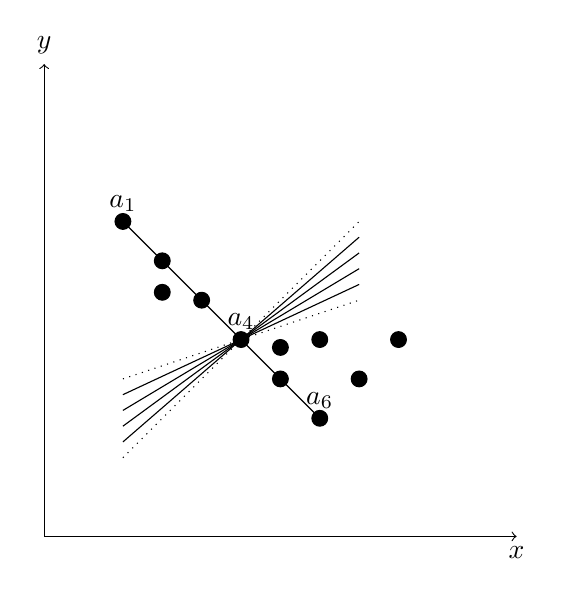
\begin{tikzpicture}      
  			%\draw[help lines,xstep=.5,ystep=.5,dashed] (0,0) grid (6,6); %Hilfsdiagramm für Koordinaten
  			%\foreach \x in {0,1 ,...,6} { \node [anchor=north] at (\x,0) {\x}; }
  			%\foreach \y in {0,1,...,6} { \node [anchor=east] at (0,\y) {\y}; }
  			
  			\draw[->,] (0,0) -- 	(6,0) node  [at end,anchor= north]{$x$}; %x axis
  			\draw[->,] (0,0) -- 	(0,6) node  [at end,anchor= south]{$y$}; %z axis
  			
  			% sorted in rising x
  			\draw[fill=black]       (1,4) circle (0.1) node (M)[above]{$a_1$}; % point M
  			\draw[fill=black]       (1.5,3.5) circle (0.1) node (M)[above right]{}; % point M
  			\draw[fill=black]       (1.5,3.1) circle (0.1) node (M)[above right]{}; % point M
  			\draw[fill=black]       (2,3) circle (0.1) node (M)[above right]{}; % point M
  			\draw[fill=black]       (2.5,2.5) circle (0.1) node (M)[above]{$a_4$}; % point M
  			\draw[fill=black]       (3,2) circle (0.1) node (M)[above right]{}; % point M
  			\draw[fill=black]       (3,2.4) circle (0.1) node (M)[above right]{}; % point M
  			\draw[fill=black]       (3.5,1.5) circle (0.1) node (M)[above]{$a_6$}; % point M
  			\draw[fill=black]       (3.5,2.5) circle (0.1) node (M)[above right]{}; % point M
  			\draw[fill=black]       (4,2) circle (0.1) node (M)[above right]{}; % point M
  			\draw[fill=black]       (4.5,2.5) circle (0.1) node (M)[above right]{}; % point M
  			
  			\draw[dotted] (1,1) --  (4,4) node []{};
  			\draw[] (1,1.2) --  (4,3.8) node []{};
  			\draw[] (1,1.4) --  (4,3.6) node []{};
  			\draw[] (1,1.6) --  (4,3.4) node []{};
  			\draw[] (1,1.8) --  (4,3.2) node []{};
  			\draw[dotted] (1,2) --  (4,3) node []{};
  			\draw[] (1,4) --  (3.5,1.5) node []{};
  			
  			\end{tikzpicture}
  			\caption{Points in image space}
  			\label{fig_Hough1}
  		\end{centering}
  	\end{minipage}\hfill
  	\begin{minipage}[t]{0.48\textwidth}
  		\begin{centering}
  			\begin{tikzpicture}      
  			%\draw[help lines,xstep=.5,ystep=.5,dashed] (0,0) grid (6,6); %Hilfsdiagramm für Koordinaten
  			%\foreach \x in {0,1 ,...,6} { \node [anchor=north] at (\x,0) {\x}; }
  			%\foreach \y in {0,1,...,6} { \node [anchor=east] at (0,\y) {\y}; }
  			
  			\draw[->,] (0,0) -- 	(6,0) node  [at end,anchor= north]{$m$}; %x axis
  			\draw[->,] (0,0) -- 	(0,6) node  [at end,anchor= south]{$b$}; %z axis
  			
  			
  			% sorted in rising x
  			\draw[fill=black]       (1.5,3) circle (0.1) node (M)[above]{$c_1$}; % point M
  			\draw[]       (1,3.5) circle (0.1) node (M)[below right]{}; % point M
  			\draw[]       (0.5,4) circle (0.1) node (M)[below right]{}; % point M
  			\draw[]       (3,2) circle (0.1) node (M)[below right]{}; % point M
  			\draw[]       (1.7,2.5) circle (0.1) node (M)[below right]{}; % point M
  			\draw[]       (3,2.7) circle (0.1) node (M)[below right]{}; % point M
  			\draw[]       (14,2.4) circle (0.1) node (M)[below right]{}; % point M
  			\draw[]       (1.8,1.5) circle (0.1) node (M)[below right]{}; % point M
  			\end{tikzpicture}
  			\caption{Lines in feature space}
  			\label{fig_Hough2}
  		\end{centering}
  	\end{minipage}
  \end{figure}
  
   \section{Distance Measurement with \ac{LIDAR}} \label{LIDAR}
   With the rapid development of lasers for optical distance measurement, today the \ac{LIDAR} technology is widely used in different fields of applications. After an introduction to the working principle of a \ac{LIDAR}, this section continuous by detailing four clustering algorithms that can be applied on the \ac{LIDAR} data. In subsection \ref{Hough3d} the Hough algorithm for the three-dimensional space is explained followed by the partition based K-Means algorithm in subsection \ref{K-means}. Hereafter, subsections \ref{Birch} and \ref{DBSCAN} explain the hierarchic \ac{BIRCH} and density based \ac{DBSCAN} algorithm respectively.\\
   
   A classification based on the transmission waveform and data processing method divides the \ac{LIDAR} technology into pulsed, continuous wave, pulse compression, moving target display, pulse Doppler and imaging \ac{LIDAR}. All of these varieties are based on the fundamental principle of a \ac{LASER}. The wavelength of the laser is in the range of ultraviolet, infrared or visible light. Typically, a wavelength of about 1000nm or less is used. One advantage that a pulsed laser has over a continuous laser is the higher light intensity for a period of time. A typical measurement cycle according to the pulsed laser method comprises three integrations. A laser pulse is emitted and the received radiation is registered via integration one. After the time $t_{pulse}$ is elapsed, in the first integration the backlight and the first part of the reflected pulse is saved. Hereafter, integration two sums up the backlight and the last part of the reflected pulse. Integration three solely measures the backlight over a certain period of time. With equation \ref{Eq_ToFdirekt2} derived in \cite{ASpieck} and in \cite{ADrie}, the quotient $Q_{ToF}$ can be calculated. The backlight or noise is subtracted by integration three from the reflected light measured in integration one and two. With the pulse length $t_{pulse}$, $t_{ToF}$ can be calculated by \eqref{Eq_ToFdirekt3}. By multiplication with the speed of light $c$, the now known value  $t_{ToF}$ results in the distance of the object from which the light was reflected.
      
    \begin{equation} 
   \label{Eq_ToFdirekt2}
   Q_{ToF}=\frac{integration2-integration3}{integration1+integration2-2*integration3}
   \end{equation}
   
   \begin{equation}
   \label{Eq_ToFdirekt3}
   t_{ToF}=t_{pulse}*Q_{ToF}
   \end{equation}
   
   \begin{equation} 
   \label{Eq_ToFdirekt1}
   d=\frac{c}{2}*t_{ToF}
   \end{equation}                                                                                                                               
   To obtain a point cloud and scan the environment of the \ac{LIDAR}, the emitted light has to be directed by some means. Different scanning methods exist of which one is a motor-driven rotation of a mirror, which reflects the laser and hereby allows sampling of the surrounding of up to 360\degree. As moving parts are part of this method, friction and therefore a reduced durability are inherent to this approach. However, because of the technical simplicity this implementation is widely used. A typical mechanical \ac{LIDAR} scanner with the aforementioned laser as a source, comprises the a servo motor as an actuator and a mirror as the rotational element.
  
   
   The segmentation of the \ac{LIDAR} data takes a vital role to extract the necessary information used for the subsequent object classification.  A number of segmentation algorithms were proposed in the last years which can be divided into direct and indirect approaches. Given a point cloud with artefacts shaped in regular geometric shapes, an example for a direct
   approach is given by the Hough transformation. Geometric parameters can be extracted directly from the point cloud data besides the segmentation process. Indirect segmentation methods apply for example progressive algorithms (over time improving approximations of a complete solutions with intermediate results \cite{ProgAlg}) on the point cloud data to compute spatial proximity and geometric derived values as for example local surface normal vectors. Common algorithms for an indirect data segmentation by clustering without feature extraction comprise methods based on partitioning, hierarchy and density. 
   
   \subsection{Hough Transform Algorithm (direct approach)} \label{Hough3d}
   The Hough Transform Algorithm for the 3D space works similar to the Hough Transform Algorithm in the 2D space which is frequently used in image feature extraction. The 2D Hough algorithm is explained in section \ref{Houghtransf}. Let a planar feature in the 3D carthesian space be described by a function F as shown in equation \ref{eq_imSpace}, it can be converted into angle information to the form in equation  \ref{eq_featSpace}.
   \begin{equation} 
   \label{eq_imSpace}
   F=ax+ by+ cz+ d= 0%\frac{c}{2}*t_{ToF}
   \end{equation} 
  \begin{equation}
   \begin{aligned} 
   \label{eq_featSpace}
    &\rho= x\cos\theta\sin\phi+ y\sin\theta\sin\phi+ z\cos\phi \\
    & \theta \in [0\degree,360\degree], \phi \in [-90\degree,90\degree]
   \end{aligned}
   \end{equation}
   
   The normal vector n of the planar feature is described by the parameters $\theta, \phi$ and $\rho$ as depicted in figure \ref{fig_HoughIm}. Accordingly, the Hough space consist of these parameters. The algorithm (accumulator) now iterates through the point cloud data and maps the possible normal vectors of each point in its feature space
   (Hough space). Hence, every time a point is on the planar feature, the density of the parameters ($\theta, \phi, \rho$) in the feature space related to n will increase. Points with a high density in the feature plane therefore represent a plane in the 3D carthesian space and the feature is extracted. However, for each point in data, there are 
   $x_\theta*x_\phi$ possibilities to be mapped in the feature space. With $y$ points in the point cloud the accumulator needs $y*x_\theta*x_\phi$ iterations to finish the process. For large databases, the process therefore requires many iterations and the computational power has to be sufficient to cluster the database in the required time frame of the application.
   \begin{figure}
   	\begin{centering}
   		\begin{tikzpicture}      
   		%\draw[help lines,xstep=.5,ystep=.5,dashed] (0,0) grid (10,10); %Hilfsdiagramm für Koordinaten
   		%\foreach \x in {0,1 ,...,10} { \node [anchor=north] at (\x,0) {\x}; }
   		%\foreach \y in {0,1,...,10} { \node [anchor=east] at (0,\y) {\y}; }
   		\draw[->,] (3,3) -- 	(3,8)     	node (z) [at end,anchor= south]{$z$}; %z axis
   		\draw[->,] (3,3) -- 	(1,1)     	node (x) [at end,anchor= north]{$x$}; %x axis
   		\draw[->,] (3,3) -- 	(8,3)     	node[at end,anchor= north]{$y$}; % y axis
   		\draw[->,] (3,3) -- 	(4,7.5)   node (n)[midway,anchor= east]{$\rho$} node[at end,anchor= east]{$n$}  ; % n axis normal vector to plane		  
   		\draw[] (4.5,5) -- 	(7.5,6)   	; % plane line
   		\draw[] (4.5,5) -- 	(2,6)     	; % bottom to right plane line
   		\draw[] (2,6) -- 	(4.5,7)     	; % bottom to left plane line
   		\draw[] (4.5,7) -- 	(7.5,6)     ; % mid to top plane line
   		\draw[dashed] (3,3) -- (3.75,2) node (xy)[] {} ; % bottom square intersecting line 
   		\draw[dashed] (2,2) -- (3.75,2) ; % bottom square left to right
   		\draw[dashed] (4.75,3) -- (3.75,2)     ; % bottom square right to top
   		\draw[dashed] (3.75,6.5) -- (3.75,2)     ; % %perpendicular to bottom suquare to plane
   		%\coordinate at (5,6.5) node {P};
   		\coordinate (origo) at (3,3); % origin coordinates coordinate system
   		\pic[draw, "$\phi$", angle radius=0.5cm, anchor= south west] {angle=xy--origo--n}; %angle phi
   		\pic[draw, "$\theta$", angle radius=0.7cm] {angle=x--origo--xy}; % angle theta
   		\end{tikzpicture}
   		\caption{A planar feature described in the 3D hough image space \cite{EnvPerc}.}
   		\label{fig_HoughIm}
   	\end{centering}
   \end{figure}

   \subsection{K-Means algorithm (partition based) }  \label{K-means}
   The K- means partitioning algorithm follows a very straight forward method and is divided into three steps. The first step is to find a center point for each cluster, which can be done randomly. The distance from each point to the center point of each cluster is calculated in a second step. In a third step, the average coordinates from each point of a cluster is calculated and defined as the new center of the according cluster. Step two and three can be iterated until a difference criterion between the former and actual cluster center is found. Therefore to reach a certain accuracy, many iterations can be necessary and the computational effort for large databases is high.
   \subsection{BIRCH Algorithm (hierarchic)} \label{Birch}
   The \ac{BIRCH} algorithm is used for very large datasets which are to be processed in a limited time with very small amount of used memory space. In most cases, one single scan of the data which is to be clustered is sufficient. Furthermore, noise is handled effectively \cite{BIRCH}.
   Based on the \ac{CF} and the hierarchical \ac{CFT}, the \ac{CF} is  defined by the triplet $(N_i, \vec{LS}, \vec{SS})$, in which $N_i$ represents the $i$ data points in the cluster, $\vec{LS}$ the sum $\sum N_i$ and $\vec{SS}$ the sum of squares $\sum N_i^2$. The cluster features can be added to each other which is expressed by equation \ref{eq_BirchMerge}.
   \begin{equation}
   \label{eq_BirchMerge}
   CF1+CF2=(N1+N2, \vec{LS1}+\vec{LS2}, \vec{SS1}+\vec{SS2})
   \end{equation}
    The \ac{CF} are stored in a \ac{CFT} with Root, Nonleaf, and Leafnotes and the MinCluster as depicted in figure \ref{fig_BIRCHTree}. B describes the maximum branches of the Nonleafes and L the maximum branches of the MinCluster. The parameter T limits the radius of the cluster. The algorithm consists of five consecutive steps. First, the nearest CF node to the new sample is found. If, second, the distance between the new sample and the CF node is less than the threshold T, insert the sample. Otherwise, and if the CF branches (MinCluster) of the leaf node are below the threshold L, insert a new MinCluster. If the threshold requirement L is not met, in a fourth step divide the leaf into two new leafs. The two MinCluster furthest away from each other are selected for the new leaf nodes. The new sample and the already given samples have to be assigned to the according leaf hereafter.
   
   The main advantage is that no iteration over the datapoints is necessary, as each datapoint is read in only once. As the \ac{CFT} only points to the data that is saved, even high amounts of data can be processed. However, due the limited \ac{CF} per node, the algorithm is prone to over segmentation and is also called a micro clustering approach. Therefore, created cluster may not represent the real world situation especially for large target objects in the measured data \cite{EnvPerc}. Additionally due to distance restriction of the \ac{CF}, the shape of the cluster data tends to be spherical for large target objects.
 
\begin{figure}
	\begin{centering}
	
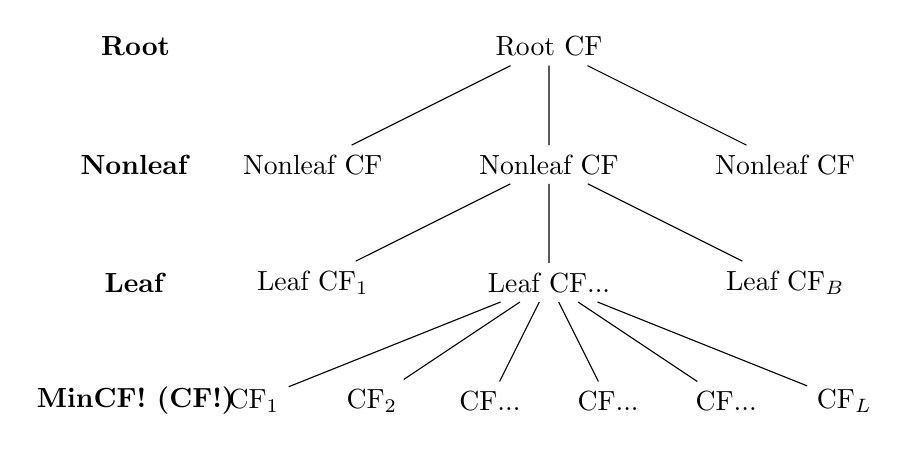
\begin{tikzpicture}[level distance=1.5cm,
level 1/.style={sibling distance=3cm},
level 2/.style={sibling distance=3cm},
level 3/.style={sibling distance=1.5cm},
level 4/.style={sibling distance=1cm}]

\node (Root) {Root CF} % Root cluster
child {node {Nonleaf CF}} % nonleaf cluster
child {node {Nonleaf CF}  % nonleaf cluster
	child {node {Leaf CF$_1$}} % leaf cluster
	child {node {Leaf CF...} % The CF nodes start below this Leaf CF
		child {node{CF$_1$} % From this node, the level describtion starts from downwards to Root
			child [grow=left] {node (q) {\textbf{Min\ac{CF}}} edge from parent[draw=none] % level description Cluster
				child [grow=up] {node (q) {\textbf{Leaf}} edge from parent[draw=none] % level description Nonleaf
					child [grow=up] {node (q) {\textbf{Nonleaf}} edge from parent[draw=none] % level description Leaf
						child [grow=up] {node (q) {\textbf{Root}} edge from parent[draw=none]}}}}} % level desctiption Root
		child {node{CF$_2$}} % cluster CF
		child {node{CF...}} % cluster CF
		child {node{CF...}} % cluster CF
		child {node{CF...}} % cluster CF
		child {node{CF$_L$}}}	% cluster CF
	child {node {Leaf CF$_B$}}} % cluster CF
child {node {Nonleaf CF}}% non leaf CF
;
\end{tikzpicture}
\caption{A \ac{CFT} derived from the \ac{BIRCH} Algorithm \cite{EnvPerc}.}
\label{fig_BIRCHTree}%Label für das Referenzieren 
\end{centering}
\end{figure}
\subsection{DBSCAN (density based)} \label{DBSCAN}
With the \ac{DBSCAN} algorithm a method is proposed with which arbitrary shaped targets can be clustered even in an environment with present noise. It is a density based approach and efficient for large spatial databases. The algorithm takes advantage of the characteristic of a shape or cluster, that the points of the cluster provide a higher density than the noise outside of a cluster. Therefore each point inside a cluster requires to have a minimum of points $MinPts$ inside its neighbourhood $Eps$. The shape of a neighbourhood is to be determined by the function of distance of two points with $dist(p,q)$, where $Eps$ is the maximum distance between two points $p,q$ to consider them as neighbours. For example for an Euclidean distance the shape of a neighbourhood would be spherical and for a Manhattan distance, the shape would be rectangular. Equation \ref{eq_DBSCANDef1} describes this relation with $N_{Eps}$ describing the $Eps$ neighbourhood and $D$ the dataset of points in a k-dimensional space to be considered.
 \begin{equation}
\label{eq_DBSCANDef1}
N_{Eps}(p)= \{q\in D |dist(p,q) \leq Eps \}
\end{equation}
A point $p$ that full fills the requirement of $MinPts$ points $q$ in its neighbourhood is considered to be directly-density-reachable with the formal definition described by equation \ref{eq_DBSCANDef2}.
\begin{equation}
\label{eq_DBSCANDef2}
p \in N_{EPS}(q) \land |N_{Eos}(q)| \geq MinPts
\end{equation}
However, because a data point $p$ at the border of a cluster may not full fill the requirement of $MinPts$ points inside its neighbourhood but is nevertheless inside the cluster, its relation to a point $q$ is defined by the expression density-reachable. A point $p$ is density-reachable, if there is a chain of points $p_1,...,p_i= q, p_n=p$ with $p_{i+1}$ directly-density-reachable from $p_i$. A third definition is required to describe the relation of two points $p$ and $q$ both at the border of a cluster. They are density-connected if a point $o \in N_{Eps}$ is density-reachable from $p$ and $q$ \cite{DBSCAN} \cite{DBSCANRev}. Figure \ref{fig_DBSCAN} depicts the aforementioned relations with the points B, A, C and N. N can be considered as noise and is unrelated to a cluster because it is not connected to another points by any given definition. The data points A are directly-density-reachable from each of the red points. The data points B and C are density-reachable from A and the other red points are density-connected to each other by the red points. The found cluster now consists of the red and yellow points.

As density based algorithms as the \ac{DBSCAN} depend essentially on the closeness $Eps$ of the data points to each other, spatially distributed cluster and varying density results in large inaccuracies \cite{ClusterOver}. Therefore, in an environment with these characteristics an adaptive value for $Eps$ is required. A linear threshold expressed with equation \ref{eq_DBSCANAdv} has been experimentally proven to be feasible. The arc length $L$ is calculated with the angle resolution $\theta$ and the distance $d_i$ and results in $Eps$ together with the precision factor $n$. Additionally, because not only the distance of points to each other, but the density of points inside a cluster can be reduced by increasing distance, the minimum of required points inside a cluster may be adapted with a linear equation related to the distance \cite{AdvancedDBSCAN}.
\begin{equation}
\begin{aligned} 
\label{eq_DBSCANAdv}
& L= \frac{\theta\pi d_i}{180}  \\
& Eps = nL
\end{aligned}
\end{equation}

 
   
   \begin{figure}
   	\begin{centering}
   		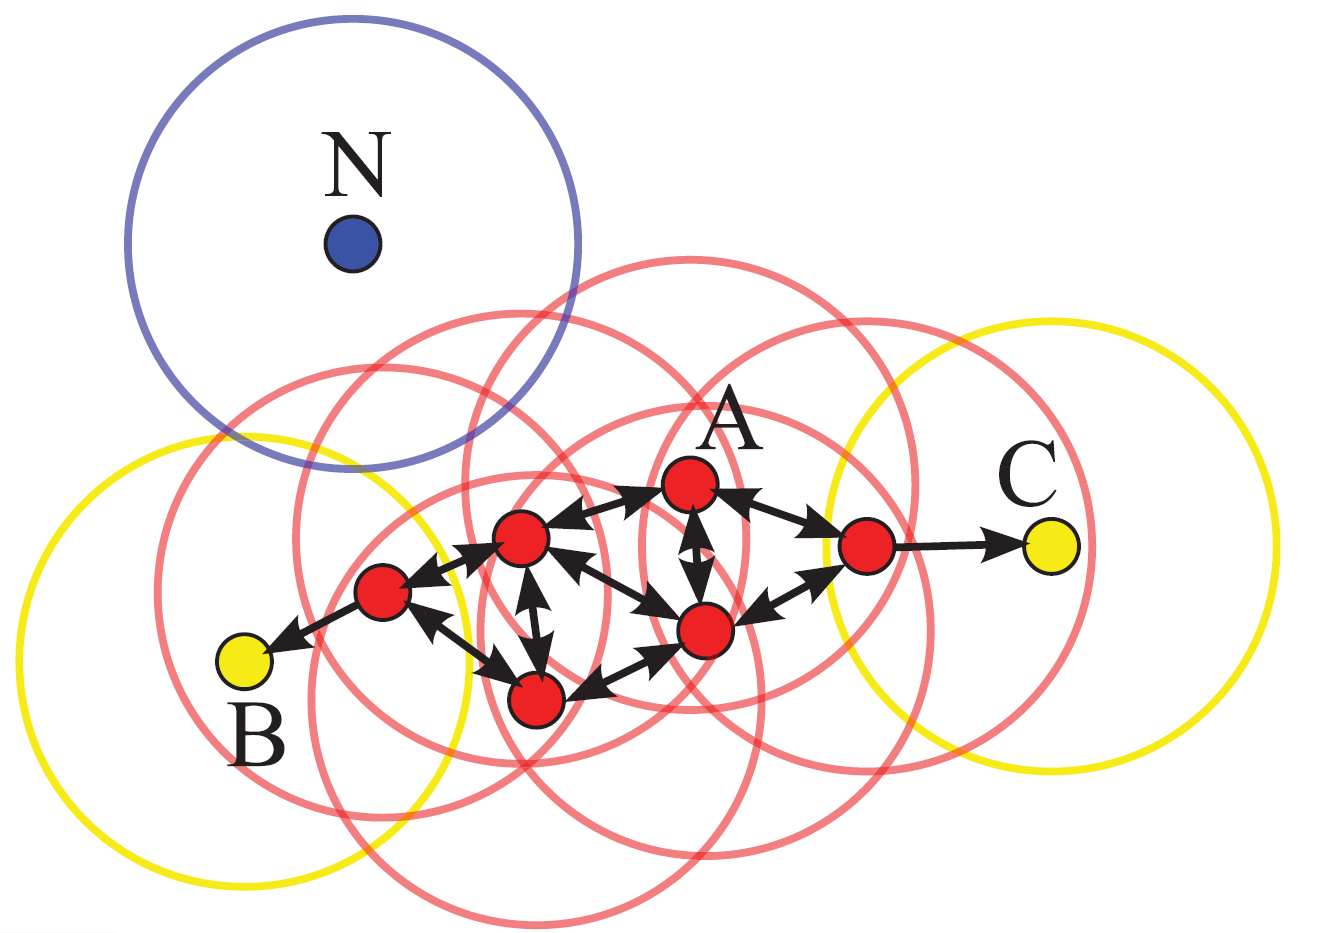
\includegraphics[width=0.5\linewidth,keepaspectratio]{Bilder/DBSCAN.png}
   		\caption{Clustered data with \ac{DBSCAN} and noise \cite{DBSCANRev}.}
   		\label{fig_DBSCAN}%Label für das Referenzieren 
   	\end{centering}
   \end{figure}
   
   
   \section{Object Detection with \ac{RADAR}} \label{RADAR}
   After an introduction to the fundamental formulas that describe \ac{RADAR} systems, this section continuous with four different approaches to filter the \ac{RADAR} data. in subsection \ref{constThresh}, a constant threshold is explained to separate noise from the signal. Continued by subsection \ref{CFARthr}, a dynamic threshold calculation is introduced which is the foundation for subsection \ref{OSthre} and \ref{SOCAthre}. In this subsections, derivatives to the afore mentioned dynamic threshold calculation are explained.\\  
   
   A millimetre wave \ac{RADAR} can estimate distances by means of electromagnetic waves with a frequency between 30GHz and 300GHz and wavelength between 1-10mm. An electromagnetic wave is emitted and reaches a possible target with the energy $S_e$ (equation \ref{eq_RADAREmit}). In equation \ref{eq_RADAREmit}, $g$ represents the antenna gain, $P_S$ the power of emittance in Watts and $r$ the distance from the antenna to the target.  
   \begin{equation}
   \label{eq_RADAREmit}
   S_e=\frac{gP_s}{4\pi r^2} \quad \quad  [\frac{W}{m^2}] % quad for spacing
   \end{equation}
   The electromagnetic wave is then reflected with the energy $S_s$ according to equation \ref{eq_RADARRec} with $r$ similar to \ref{eq_RADAREmit} and $A_e$ being the RADAR cross section calculated by \ref{eq_RADARCross} \cite{Funk}. 
   \begin{equation}
   \label{eq_RADARRec}
   S_s=\frac{A_eS_e}{4\pi r^2} \quad \quad  [\frac{W}{m^2}]
   \end{equation}
   Equation \ref{eq_RADARCross} can be described as the ratio of the target surface $A_{pl}$ to the wavelength $\gamma$ of the emitted wavelength. Therefore, the larger the wavelength and the smaller the surface area of the target object, the smaller the reflected energy and the higher the signal to noise ration. For practical considerations, in most cases values with sufficient accuracy can be calculated by approximating the target area as planar\cite{Funk}. For further specification, the power of the radiation depends on the size, shape and material of the target \cite{EnvPerc}.
   \begin{equation}
   \label{eq_RADARCross}
   A_e=4\pi\frac{A_{pl}^2}{\gamma^2} \quad \quad  [m]
   \end{equation}
   
   Two operational principles can be distinguished of which the first is the continuous wave system RADAR and the second the pulse system RADAR. In the continuous wave system the reflectance of the target object is received during the emittance of waves. In the pulsed system, a wave is emitted intermittently and during the emittance breaks, the reflectance is received. Inherent to both systems is the importance of signal processing to increase the target detection in a non uniform environment and improve target position estimation. 
   
   \subsection{Constant Threshold} \label{constThresh}
   The most straight forward approach is to empirically determine a threshold to separate the objects reflectance signal from the noise and clutter of the measurement. The higher the threshold, the lower the probability of false alarms becomes. However, with a high threshold, the probability to ignore targets becomes higher, too. Therefore, the level of the threshold is vital in this approach. To add further robustness, several measurements of the same object can be compared and only data points which are consistently above the threshold can be specified as an object representation. Hence, the more measurements are made, the higher is the certainty with which objects can be determined. In figure \ref{fig_ConseqRADAR}, four different measurements of the same scene are depicted. On the first axis the time $t$ is plotted and the second axis represents the reflected signal strength $U_E$. Only the corresponding value of $t_x$ to $t_x+\Delta t_x$ is above the threshold $U_S$ in all measurements. Thus, a target reflectance can be associated to this period of time with some certainty. In contrast, the time $t_y$ to $t_y+\Delta t_y$ exceeds the threshold only once and can be classified as noise or clutter \cite{Funk}. Due to the fixed threshold, environments with changing noise intensity results in varying probabilities for false alarms. Additionally, the targets reflectance may change due to positional deviations and resulting surface area changes and thus further raise the false alarm probability. 
   \begin{figure}
   	\begin{centering}
   		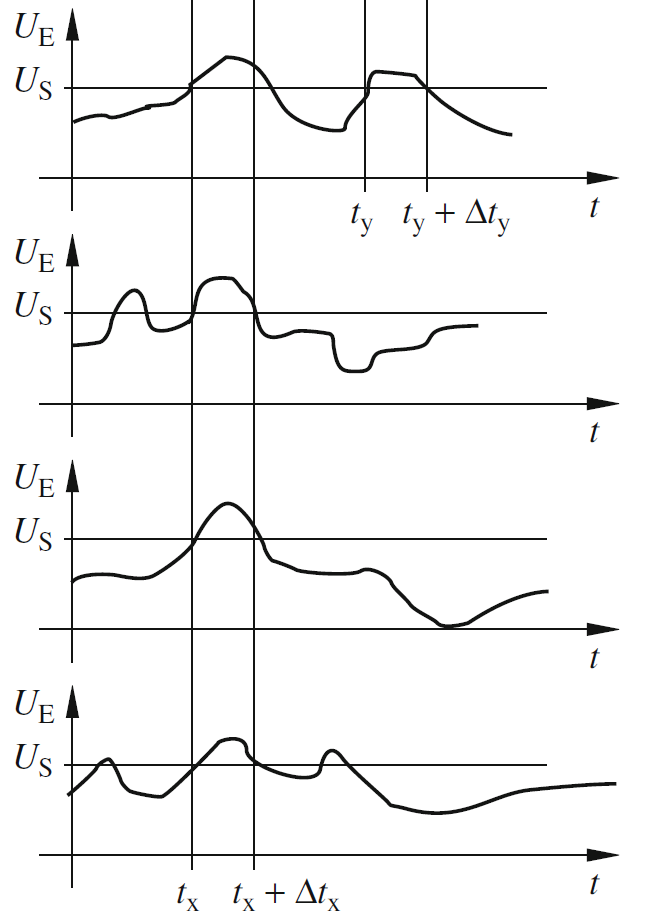
\includegraphics[width=5cm,keepaspectratio]{Bilder/ConseqRADAR.png}
   		\caption{Four datasets to distinguish the target from noise and clutter \cite{Funk}.}
   		\label{fig_ConseqRADAR}%Label für das Referenzieren 
   	\end{centering}
   \end{figure}
       
   \subsection{\ac{CFAR}} \label{CFARthr}
    By taking the \ac{SNR} as a threshold rather than the absolute value of the signal, an adaptive signal threshold can be realized and the probability for an false alarm is reduced even in situations with a high noise signal strength. First, the noise of the measurement has to be determined and normalized. Specifically in naval applications, the noise can be approximated with different \acp{PDF} of which one is the Rayleigh distribution \cite{SeaClutter}. The \ac{PDF} of the Rayleigh distribution is shown in equation \ref{eq_Ray} with the noise $x$ and $b$ proportional to the mean of the noise $\mu$ according to \ref{eq_RayFac}.  
   \begin{equation}
   \label{eq_Ray}
   P(x)=\frac{x}{b}^{-\frac{x^2}{2+b^2}}
   \end{equation}
   \begin{equation}
   b=\sqrt{\frac{2}{\pi}}+\mu
   \label{eq_RayFac}
   \end{equation}
   To express equation \ref{eq_Ray} independent of the noise level, $b$ can be substituted by $y=x/b$ which results in equation \ref{eq_RayUn}. \begin{equation}
   \label{eq_RayUn}
   P(y)=y^{-\frac{y^2}{2}}
   \end{equation} 
   The probability for a value $y$ is now only dependent on the \ac{SNR} of the target signal to the mean noise of the environment. A system diagram of the necessary operations is provided by figure \ref{fig_CFAR}. A mean value $\mu$ of the noise is calculated with one or more sampling pulses and compared with the input signal $x$. It is not required to take additional sampling pulses to the already taken samples, because the noise can be extracted from the present measurements. This can be either done by dividing the area of interest into cells and measure the noise in cells surrounding the target by assuming that these cells only consist of noise \cite{SigProcRADAR}. Another approach is to use the measured signal levels before and after the target reflectance. Therefore, it has to be assumed that the area before and after the target represents solely noise \cite{EnvPerc}. After the noise extraction, the mean value $\mu$ of the noise is estimated and compared to the input signal $x$. The hereby resulting value $y$ is given to the detector, which compares the value to the  \ac{SNR} threshold $U_0$. Either the signal is above the determined threshold and the output results in a target signal (one) or the threshold is not exceeded and therefore no target signal is detected (zero). The probability for a false alarm therefore can be set through the threshold.
   \begin{figure}
   	\begin{centering}
   		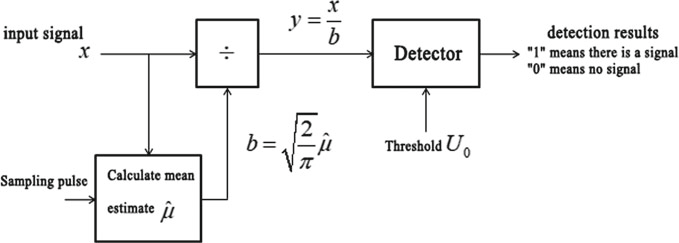
\includegraphics[width=0.75\linewidth,keepaspectratio]{Bilder/CFAR.png}
   		\caption{Single target \ac{CFAR} with fixed threshold  \cite{EnvPerc}.}
   		\label{fig_CFAR}%Label für das Referenzieren 
   	\end{centering}
   \end{figure}
  
   
   \subsection{\ac{OS-CFAR}} \label{OSthre}
   Considering the possibility of different noise and clutter levels in the sample, the aforementioned method with a very basic noise calculation approach can reach its limits in real world applications. The method as proposed in \cite{AdvCFAR} resembles the ideas of image processing. More specific, the clutter and noise power estimation that for example derives one value by averaging the whole noise sample is replaced by an arithmetic averaging procedure that is applied already in image processing applications. Especially for dense target situations, the proposed method provides advanced target extraction capabilities. The most significant change to common \ac{CFAR} approaches is the application of order statistics to derive a noise value close to the field of interest. The field of interest is divided into cells of which the centre cell is called \ac{CUT} as depicted in figure \ref{fig_StatCFAR}. The aim is the decision whether there is a target present in the cell or not by comparing the signal strength of the cell with its surrounding cells. The green cells right and left of the \ac{CUT} are called guard cells and are lined up in a one dimensional space in this example. In a three dimensional application they would build a sphere around the \ac{CUT} accordingly. They are ignored in the measurement, because the signal energy can affect adjacent cells and may effect the noise calculation. The signal strength of the cells $x_1...x_N$ and $y_1...y_M$ are most important for the noise calculation and are processed by the order statistic process in such a way that $x_{(1)}\leq... \leq x_{(k)}\leq... \leq x_{(N)}$ and $y_{(1)}\leq... \leq y_{(k)}\leq... \leq y_{(N)}$. Hereafter, these values can be described by a \ac{PDF} of order statistics. One value $x_k, \quad k \in \{1,2,...,N\}$ or $y_k, \quad k \in \{1,2,...,M\}$ is then selected and used as an estimation for the average noise power $Z$ as shown in equation \ref{eq_AvClut}.
   \begin{equation}
   Z= X_{(k)}
   \label{eq_AvClut}
   \end{equation}
   By scaling $Z$ with the factor $T$, an adaptive threshold $S$ for the comparator is found (equation \ref{eq_thres}). 
   \begin{equation}
   S= TZ
   \label{eq_thres}
   \end{equation}
   In figure \ref{fig_StatCFAR}, $\alpha$ resembles the scaling factor $T$ of equation \ref{eq_thres} and with $\beta$ the threshold can be further adjusted. A comparator thereafter compares the value of the \ac{CUT} to the threshold and the decision is made, whether there is a target (one) or only noise (zero) in the according cell. The algorithm then iterates through the cells until each cell is set to zero or one. The advantage of multi target detection in this approach resulting from the independency of the mean value of the clutter comes by the disadvantage of high computational effort to calculate the threshold. The probability that a random noise variable $Y_0$ of the \ac{CUT} is interpreted as an echo of the target can be expressed with equation \ref{eq_OrdStat}. To obtain a required false alarm rate, this equation has to be solved to derive the scaling factor $T$. 
   \begin{equation}
   P_{fa}=P[Y_0\geq TZ]
   \label{eq_OrdStat}
   \end{equation}
   As aforementioned, in sea borne applications, the Rayleigh function can be used as an estimation to clutter and therefore describes the \ac{PDF} of $Y_0$ sufficiently. However to proof the independency of the mean value of all noise values in the threshold calculation, a simple exponential distribution for the noise following $1/\mu e^{-x/\mu}$ is sufficient. The \ac{PDF} of $Z=x_k$ is shown by equation \ref{eq_OrdEq}.
   \begin{equation}
   P_{x_k}= \frac{k}{\mu_{N,k}}{e^{\frac{-x}{\mu}}}^{N-k+1}({1-e^{\frac{-x}{\mu}}}^{k-1})
   \label{eq_OrdEq}
   \end{equation}
   As both \ac{PDF} of $Y_0$ and $Z=x_{(k)}$ are known, the scaling factor $T$ can be calculated for a required false alarm rate $P_{fa}$ with equation \ref{eq_OrdStat} which results in equation \ref{eq_OrdP}.
   \begin{equation}
   P_{fa}= k_{N,k}\frac{(k-1)!(T+N-k)!}{(T+N)!}
   \label{eq_OrdP}
   \end{equation}
   It has to be noted that with this equation, the probability for a false alarm no longer depends on the mean value $\mu$ but solely on the scaling factor $T$ the fixed value $N$ or $M$ describing the number of the sample cells and the sample index $k$. For a fixed false alarm rate the literature proposes values for the threshold $T$ to limit the computational effort to derive these values \cite{AdvCFAR}.
	\begin{figure}
		\begin{centering}
			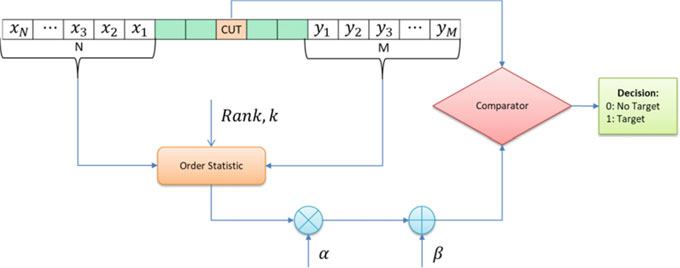
\includegraphics[width=0.6\linewidth,keepaspectratio]{Bilder/StatCFAR.png}
			\caption{Multi target \ac{OS-CFAR}, threshold calculated by ordered statistics \cite{SigProcRADAR}.}
			\label{fig_StatCFAR}%Label für das Referenzieren 
		\end{centering}
	\end{figure}
 
    \subsection{\ac{SOCA-CFAR}} \label{SOCAthre}
   The \ac{SOCA-CFAR} algorithm is a variation of the \ac{CFAR} algorithm and takes the lowest mean value of the cells right and left to the \ac{CUT} \cite{SigProcRADAR}. Therefore, the chance to detect targets with low energy is high and the computational effort moderate. That comes with the back draw of a higher false alarm detection rate. In figure \ref{fig_SOCACFAR} the difference to other algorithms that are based on the \ac{CFAR} method becomes clear with the orange box that decides in favour of the lowest mean value of $x_i$ and $y_i$. This is expressed by equation \ref{eq_SOCA}.% The other variables in the figure resemble figure \ref{fig_StatCFAR}. 
   
   
   
   \begin{equation}
   Z= \min (\frac{1}{N}\sum_{i=1}^{N}x_i,\frac{1}{M}\sum_{i=1}^{M}y_i)
   \label{eq_SOCA}
   \end{equation}
   
   \begin{figure}
   	\begin{centering}
   		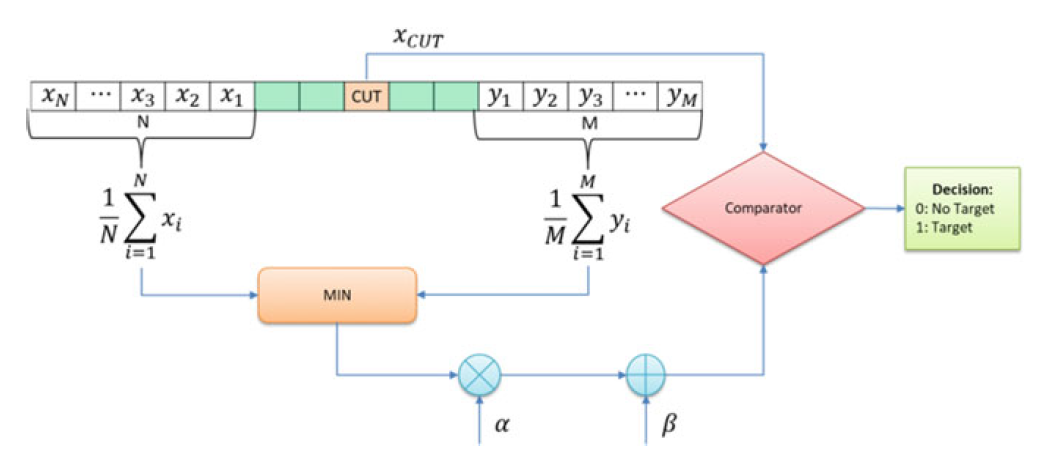
\includegraphics[width=0.6\linewidth,keepaspectratio]{Bilder/SOCACFAR.png}
   		\caption{\ac{SOCA-CFAR}, threshold calculated by average \cite{SigProcRADAR}.}
   		\label{fig_SOCACFAR}%Label für das Referenzieren 
   	\end{centering}
   \end{figure}

  \chapter{Implementation} \label{Impl}
The implementation of the system is oriented at following the V-Modell. In section \ref{Require}, the requirements of the designed system are defined. This section is followed by a description of the system architecture of the vessels \ac{GNC} system and peripherals in \ref{Archi}. The part of the architecture that is further detailed in the implementation is described hereafter. The system specification in section \ref{Spec} discusses the possible hardware, the simulation environment and the software framework used to realize the defined architecture. The software modules and its interdependencies both for the simulation and the software framework are defined in section \ref{ModuleDes} and are followed by a more detailed description and the implementation in section \ref{ModuleImp}. 

\section{Requirements}\label{Require}
 This section describes the requirements that derive from the use case of the system. The requirements are separated in the three main categories safety considerations in subsection \ref{Regulations} and hardware and software requirements in subsection \ref{ReqHardSoft}.
 \subsection{Regulations and safety}\label{Regulations}
 \begin{figure}[h]
 	\centering
 	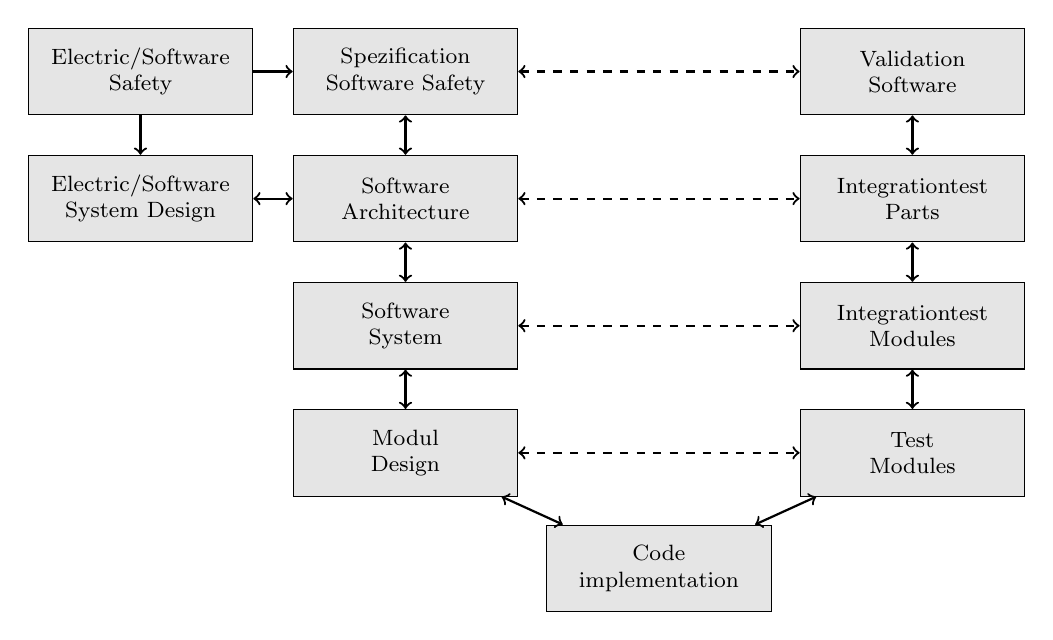
\begin{tikzpicture}
 	[node distance = 1cm, auto,font=\footnotesize,
 	% STYLES
 	every node/.style={node distance=3cm},
 	% The comment style is used to describe the characteristics of each force
 	comment/.style={rectangle, inner sep= 5pt, text width=4cm, node distance=0.25cm},
 	% The force style is used to draw the forces' name
 	force/.style={rectangle, draw, fill=black!10, inner sep=5pt, text width=2.5cm, minimum height=1.1cm,  text badly centered}]
 	
 	% V model box centre
 	\node [force,] (Code) {Code\\implementation};
 	%left
 	\node [force, above left = 0.5cm of Code] (Modul) {Modul\\Design};
 	\node [force, above = 0.5cm of Modul] (System) {Software\\System};
 	\node [force, above = 0.5cm of System] (Archi) {Software\\Architecture};
 	\node [force, above = 0.5cm of Archi] (Spezi) {Spezification\\Software Safety};
 	%right
 	\node [force, above right = 0.5cm of Code] (Modultest) {Test\\Modules};
 	\node [force, above = 0.5cm of Modultest] (Integration) {Integrationtest\\Modules};
 	\node [force, above = 0.5cm of Integration] (Integrationparts) {Integrationtest\\Parts};
 	\node [force, above = 0.5cm of Integrationparts] (Validation) {Validation\\Software};
 	%left of v modell
 	\node [force, left = 0.5cm of Spezi] (Req) {Electric/Software\\Safety};
 	\node [force, left = 0.5cm of Archi] (ArchiEl) {Electric/Software\\System Design};
 	% Draw the links between sensor forces, HMI and Actuators
 	\path[<->,thick]
 	% Vmodell and one addition at end
 	(Code) edge (Modul)
 	(Modul) edge (System)
 	(System) edge (Archi)
 	(Archi) edge (Spezi)
 	(Code) edge (Modultest)
 	(Modultest) edge (Integration)
 	(Integration) edge (Integrationparts)
 	(Integrationparts) edge (Validation)
 	(ArchiEl) edge (Archi);
 	%dotted lines of Vmodell
 	\path[<->,thick, dashed]
 	(Modul) edge (Modultest)
 	(System) edge (Integration)
 	(Archi) edge (Integrationparts)
 	(Spezi) edge (Validation);
 	% Draw lines right and left 
 	\path[->,thick]
 	(Req) edge (Spezi)
 	(Req) edge (ArchiEl);
 	
 	\end{tikzpicture} 
 	\caption{Systematic development of safety related software with the V-Model after \cite{DIN_1}.}
 	\label{fig_VModel}
 \end{figure}
 The design of a technical system has to be conducted by taking into account technical regulations. Both the EU and \ac{IMO} developed regulations for the requirements of testing \ac{MASS}. Among the regulations in the interim guidelines of the \ac{IMO} is the demand for an adequate human-system interface and a human centred design of a \ac{MASS}. Furthermore, information that is related to the vessels internal state and the data upon which the automated system judges the scene should be made available to any personnel involved in the \ac{MASS} trial \cite{IMO_MASS}. The regulation published by the EU takes into consideration the aforementioned regulation of the \ac{IMO} and highlights the  ability of the applicant of the \ac{MASS} trial to maintain a meaningful human control at any time during the test or trial with the ability to abort the trial \cite{EU_MASS}.\\
 
 Regarding the detailed design process, there are many organizations that develop standards for safety related software with the \ac{IEEE} and the \ac{IEC} considered as the most important organizations \cite{OverviewReg}. For more detailed specifications of the software requirements in programmable electronic safety related systems in Germany, the \ac{VDE} 0803-3 \cite{DIN_3} can be acquired which is related to \ac{IEC} 61508. Section 7.1 to 7.9 describe the requirements of a software safety life cycle. General information are given (7.1) and safety requirements specified (7.2). The validation of software is described (7.3) and the software development process related to safety aspects explained (7.4). The document continuous with the integration of software and electronic parts (7.5), modification processes (7.6), the software validation (7.7) and software modification (7.8) and verification (7.9). It is stated, that every model of a software safety life cycle that full fills the requirements of the document is allowed to be used with an example given by the V-Model as depicted in figure \ref{fig_VModel}. The figure describes from the upper left to the upper right the states of a development process related to the safety of software and it becomes clear, that embedding this model in a traditional V-model development process is possible. First, the electrical and software safety requirements are determined to design the electrical and software system upon which the software architecture relies. Also, the specification of the software safety can be derived from this requirements. During these steps, the software is validated and integrations tests of the software architecture are defined. The software system and module design takes place hereafter with the integration test and module test specified and applied simultaneously. The most detailed level of the design is the code implementation. The model as proposed in \ac{VDE} 0803-3 is intended to be applied on large projects, therefore steps can be merged for the application in small projects.\\
 
 Of special interests is section 7.4 in this document as it details the software design and development process with subsection 7.4.3 specifying the requirements for the design of a software architecture. The design of the system should be without faults in the concept, easily comprehensible and display a deterministic behaviour. The implementation of the design is required to be testable and has to be fault tolerant even in the case of external events. The responsibility for the software as well as the architecture of the design and modifications shall be documented (7.4.3.1-3). The document is continued by subsection 7.4.5 comprising the requirements for a detailed software system design. The responsibility for the software as well as the intended design of the system with related electrical parts and a plan for the safety validation of the system has to be documented (7.4.5.1-2). The software shall be programmed in such a way, that a modular, testable and changeable code is obtained and every system is divided into several more detailed submodules (7.4.5.3-4). Tests for the integration shall be specified in order to full fill the required safety integrity level. Every software code that is implemented shall be tested as specified in section 7.4.6.\\
  
 It is noted, that an according regulation for the development and use of programmable electronic systems in marine applications \cite{ISO} by the \ac{ISO} exists but is not used in favour for the more specific \ac{IEC} 61508 , which is referred to in the \ac{ISO} document for detailed information regarding the design process \cite{LearningAuto}.
 
 \subsection{Hardware and software} \label{ReqHardSoft}
 To enable a \ac{USV} to percept its environment, suitable sensors have to be found and ideally fused into a fault resistant representation of a present scene by the navigation subsystem.  The navigation subsystem that integrates this sensors is required to be modular to allow the system to be updated independently from other subsystems and thus provide situational awareness in changing scenes. The exchange of information with other subsystems should be ensured and a focus has to be laid on the user of the system \cite{ReqNav}. The resulting data of the navigation subsystem can be utilized in a subsequent step to control the \ac{USV} actuators in a way that serves the objectives of the planned mission. Different sensors are proposed to be utilized in a \ac{GNC} system \cite{Liu2016}. The navigation subsystem is supposed to detect obstacles and determines its position both globally and in relation to the \ac{USV}. Therefore, for long range obstacle detection, \ac{RADAR} is most suitable whereas for short distances and a higher distance resolution and accuracy \ac{LIDAR} serves the purpose. To classify objects, cameras can be used. At very close range, ultrasonic sensors are an affordable solution for obstacle detection. The global position of a \ac{USV} can be determined by \ac{GNSS} \cite{EnvPerc}. To synchronize the mission goals with the control centre a connection to the guidance subsystem is required. Furthermore, to archive given control objectives, the influences of environmental disturbances have to be measured by a wind gauge which provides both wind direction and velocity. A water speed sensor and a three dimensional \ac{IMU} serves as a feedback for the control subsystem. Ideally, the sensors can be connected to a system which allows data to be manipulated, broadcasted and send to a control station on request.\\
 
 \section{System Architecture}\label{Archi}
 
 Figure \ref{fig_systemGNC} incorporates a comprehensive system diagram of a vessels \ac{GNC} system with a software framework functioning as the middleware on a processor unit. The peripheral sensors are connected to the interface of the processor unit. The sensors data can be filtered and processed to such an extent that they suffice the data rate to the control centre and can be send to it via a connection of choice. A \ac{HMI} connected to the control centre provides the possibility to send instructions to the operating system of the vessel and thus allow the full control over the system. Consequently, a connection to the actuator control enables the applicant to access relevant functions. The actuators sensors provide the control subsystem and the control centre with data of its operational status. The system architecture as depicted allows for the selection of either real sensors or virtual sensors in conjunction with a simulation environment. The simulation can be run on a different processing unit than the software framework. However, given sufficient processing power, calculations for both systems can be conducted on one system as well.
  
 \begin{figure}[h]
 	\centering
 	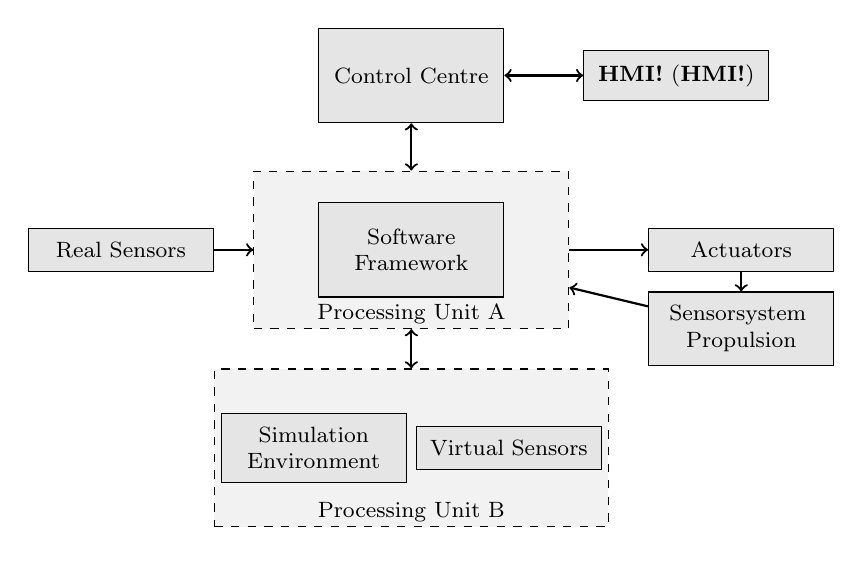
\begin{tikzpicture}
 	[node distance = 1cm, auto,font=\footnotesize,
 	% STYLES
 	every node/.style={node distance=3cm},
 	% The comment style is used to describe the characteristics of each force
 	comment/.style={rectangle, inner sep= 5pt, text width=4cm, node distance=0.25cm},
 	% The force style is used to draw the forces' name
 	force/.style={rectangle, draw, fill=black!10, inner sep=5pt, text width=2cm, text badly centered}]
 	
 	% Linux box with comment
 	\node [rectangle, draw, fill=black!5, minimum height=2cm, minimum width=4cm, dashed ] (Linux){Linux};
 	\node [comment, below=-0.5 of Linux, text centered] (comment-Linux) {Processing Unit A};
 
 	
 	% ROS box
 	\node [force,minimum height=1.2cm] (ROS) {Software\\Framework};
 	
 	% Sensor boxes
 	\node [force, left= 0.5 of Linux] (RealSensors) {Real Sensors};
 	
 	% Control centre box
 	\node [force,minimum height=1.2cm, above= 1cm of ROS] (Control) {Control Centre};
 	\draw [<->,thick](Control) -- (Linux) node [] {};
 	
 	% HMI
 	\node [force, right=1cm of Control](Human) {\ac{HMI}};
 	\draw [<->,thick](Control) -- (Human) node [] {};
 	
 	% Acutators
 	\node [force, right=1cm of Linux](Actuators) {Actuators};
 	 	
 	% Actuators sensor
 	\node [force, right=1cm of Linux, below= 0.25cm of Actuators](Propulsion) {Sensorsystem \newline Propulsion};
 	\draw [->,thick](Propulsion) -- (Linux) node [] {};
 	\draw [<-,thick](Propulsion) -- (Actuators) node [] {};
 	
 	% ComputerB
 	\node [rectangle, draw, fill=black!5, minimum height=2cm, minimum width=5cm, dashed, below =0.5cm of Linux ] (ComputerBl){};
 	\node [comment, below=-0.5 of ComputerBl, text centered] (comment-ComputerBl) {Processing Unit B};
 	\draw [<->, thick] (ComputerBl) -- (Linux) node []{};
 	
 	% Unity, Sensor box
 	\node [force,left= -2.45cm of ComputerBl] (Unity) {Simulation Environment};
 	\node [force,right=-2.45cm of ComputerBl] (Sensor) {Virtual Sensors};
 	
 	% Draw the links between sensor forces, HMI and Actuators
 	\path[->,thick]
 	(RealSensors) edge (Linux)
 	(Linux) edge (Actuators);

 	\end{tikzpicture} 
 	\caption{System diagram of the \ac{GNC} system}
 	\label{fig_systemGNC}
  \end{figure}

\section{System Specification} \label{Spec}
Referring to the designed system architecture in section \ref{Archi}, in this section the described systems of the architecture are specified. A focus is on the peripheral devices and the processing unit, that are outlined in subsection \ref{PeriDev}, followed by the selection of a central software framework in subsection \ref{Softframe}. Finally, the virtual environment is specified in subsection \ref{virtuenv}.

\subsection{Peripheral Devices and Central Processing Unit} \label{PeriDev}
The sensors described in the following are not implemented and used in an experimental verification but its defined characteristics are important for the subsequent design and implementation of the virtual sensors. They were however chosen with respect to the appliance at hand and an implementation in a real environment is encouraged. The choice of sensors is considerably reduced by the exclusion of proprietary interfaces as these can not be connected to a third party or open source solution and thus allow only very restricted access to the sensors data. An example is given by \ac{RADAR} solutions which almost always relay on the manufacturers choice of displays and therefore do not allow the data to be filtered, clustered or otherwise manipulated. Additionally a \ac{SDK} can be bought only on request, with not further specified predefined functions and executable only on the manufacturers choice of operating system. Due to this restrictions and the recent progress in solid state \ac{RADAR} solutions in the automotive field \cite{ResRADAR}, it has to be taken into consideration to use such a sensor in addition to a \ac{LIDAR} system.\\

The Aptive ESR 2.5 \cite{AptivESR} is such a automotive \ac{RADAR} sensor. It applies a millimetre wave radiation, this having a wavelength of around 80Ghz, to the environment and thereby senses up to 64 targets within a distance of 174m in long range mode. In addition to the long range mode with a \ac{FOV} of $\pm10^{\circ}$, a mid range mode with a range of 60m and a \ac{FOV} of $\pm45^{\circ}$ provides a higher degree of spatial width. The Aptive ESR 2.5 can be integrated into \ac{ROS} with an \ac{API} for \ac{CAN} provided by the company AutonomousStuff. Additionally to the \ac{CAN} interface which only provides data about extracted obstacles, an Ethernet interface gives access to the raw data of the \ac{RADAR}. To ensure the detection of obstacles further away, the Garmin GMR Fantom 54 \ac{RADAR} is used. It radiates with a power of 50W and has a range from 6m to 72 nautical miles. For closer distances of up to 100m , the Velodyne Puck \cite{VelodynePuck} provides a 3D point cloud of environmental objects with 300000 points per second and for ranges of up to 7.5m, the SEN0313 Ultrasonic sensor \cite{UltrasonicA01} gives access to analogue distance measurements. The BFS-U3-13Y3C-C 1.3MP Blackfly camera from the manufacturer Flirr \cite{Blackfly} allows for the classification of detected objects. The MTi-680G by XSens \cite{XSens}, an integrated \ac{IMU} and \ac{GNSS} unit, allows vessel localization and movement detection. Wind speed and direction can be measured with the WS200-UMB ultrasonic anemometer by Lufft \cite{Lufft}. The advantage of an ultrasonic wind gauge solution can be found in the absence of moving parts and thus an extended lifecycle. A wireless transmission to additional devices in the network is realized by the FL WLAN 1101 by Phoenix Contact \cite{Phoenix_WLAN}. An overview of suitable sensors is given in table \ref{tab_sensor}. In the table, the sensor type is horizontally followed by the product name of the chosen sensor and an estimated price as well as the interface the sensor uses to transmit data.\\

To integrate the sensors and connect its data, a central hardware solution has to be found. The Jetson AGX Xavier hardware specifications qualify it as the central data processing unit. The Xavier Development Kit provides a development platform with many standard hardware interfaces that results in a highly flexible and extensible platform for rapid prototyping. It uses a maximum power of 30W for its own supply and can supply external peripheral devices with an overall power of 35W. The Xavier Development Kit can be interfaced via USB, UART, I2C, CSI-2, Ethernet and a variety of other ports. It is run by a derivative of the operating system Linux Ubuntu. As the hardware platform hosts a powerful \ac{GPU} with according libraries such as OpenCV and TensorRT and a Multimedia \ac{API}, it is a suitable solution for sensor integration and data processing \cite{Xavier}.

\begin{table}[H]
	 \centering	
		\caption{Sensors for environment detection}
		\begin{tabular}{l l l } 
			\toprule
			Type  & Name  & Interface \\[0.25ex]
			\midrule
			RADAR&Aptive ESR 2.5 & CAN/Ethernet\\	
			RADAR & GMR Fantom 54 & Ethernet \\	
			LIDAR & Velodyne Puck & Ethernet \\	
			IMU &\multirow{3}{*}{MTi-680G}& \\  
			GNSS & &CAN\\
			Velocity&& \\
			Windspeed&WS200-UMB &  RS485\\ 
			Camera &Blackfly 1.3 MP& USB 3.1\\
			Processor & Jetson AGX Xavier  & various\\	
			Ultrasonic  & SEN0313  &  digital\\	
			WLAN & FL WLAN 1101& Ethernet \\
			\bottomrule
		\end{tabular}
	\label{tab_sensor}
\end{table}

\subsection{Software Framework} \label{Softframe}

To integrate the sensor and provide a middleware to execute the \ac{GNC} system, the frameworks \ac{ROS}, \ac{CARACAS} and \ac{MOOS-IvP} are taken into consideration. These system platforms facilitates the effort to program the required functions with predefined libraries and communication structures. 
\begin{itemize}
	\item The \ac{CARACAS} architecture is available on request for research projects and is potentially applicable on diverse robotic systems. The system is divided into three agents that interact with each other and a data storage that hosts a world model. The objective of the agents is to provide the robotic system with the capabilities of both deterministic reactions to unanticipated occurrences and re-planning in the event of changes in goals and resources. The focus therefore is on the guidance subsystem of the \ac{GNC} system \cite{CARACAS}.
	\item \ac{MOOS-IvP} is an open source project and specifically intended for the application in unmanned marine vehicles. An autonomy system, which can be referred to as the guidance subsystem, runs the autonomous decision making helmet \ac{MOOS-IvP} which is connected with an input to the data of a navigation subsystem and with an output of data of the control system (figure \ref{fig_MOOS}). Therefore, it is decoupled from the platforms hardware and does not require any specification of how the navigation and control subsystem is implemented \cite{MOOS}.
	\item  \ac{ROS} is an open source software which is developed with the objectives of modularity, usage of a peer to peer structure and being based on tools. A low level device control provides drivers for peripheral devices and a hardware independent architecture allows \ac{ROS} to be run on a wide variety of devices. Community based libraries provide methods for sensor data processing and visualization, obstacle detection, mapping and path finding \cite{ROS}. As the sensor integration into the \ac{GNC} system is vital in the design of a new robotic platform, \ac{ROS} can be evaluated as a middleware software.
\end{itemize}	

\begin{figure}
	\begin{centering}
		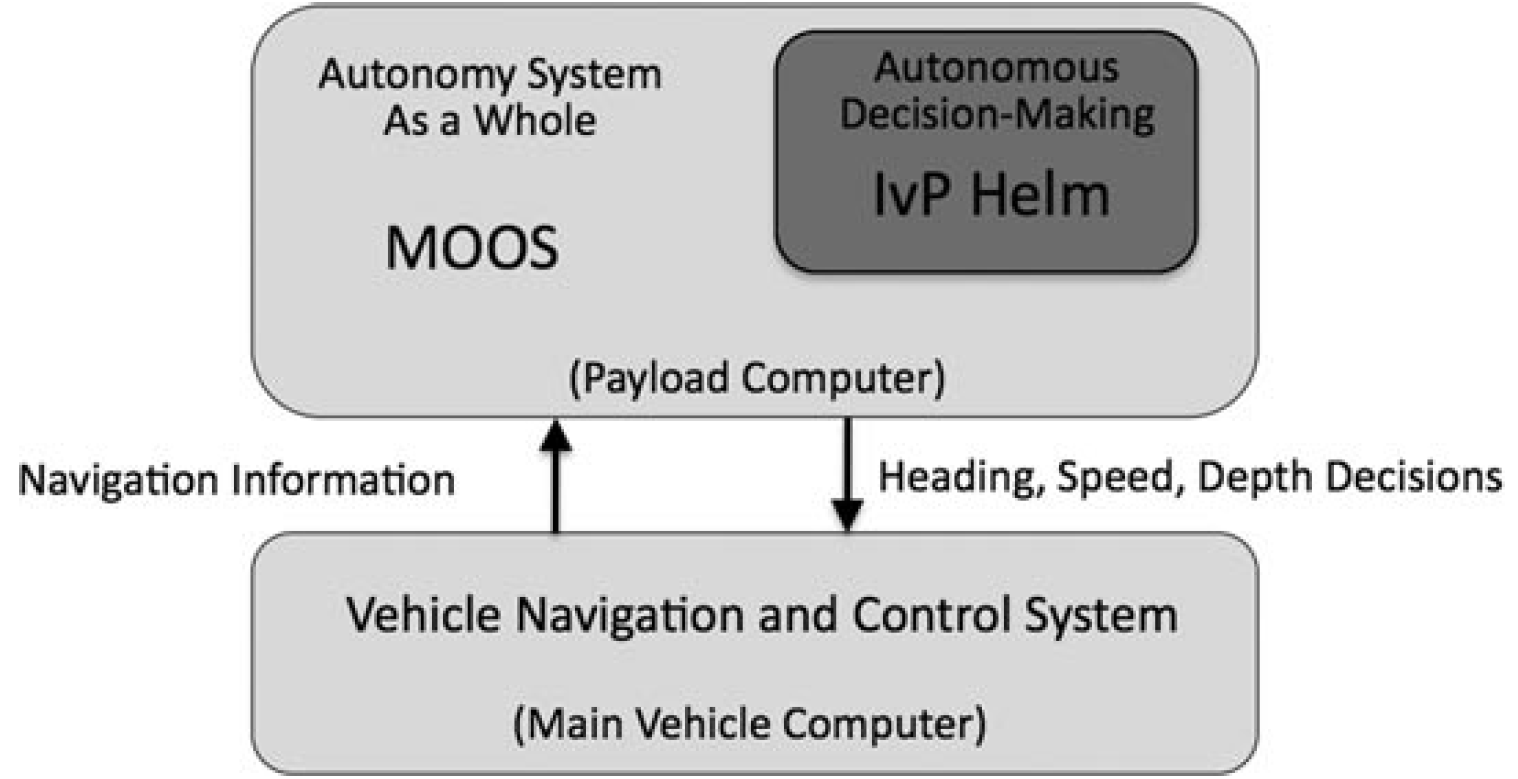
\includegraphics[width=10cm,keepaspectratio]{Bilder/MOOS.PNG}
		\caption{System diagram of the \ac{MOOS-IvP} architecture after \cite{MOOS}. The navigation and control system is physically decoupled from the autonomy system and is not further specified.}
		\label{fig_MOOS}%Label für das Referenzieren 
	\end{centering}
\end{figure}

With two different implementations of  \ac{ROS}, namely ROS1 and ROS2, the choice has to be made which of them is best suited to the application at hand. Developed since 2007, ROS1 provides a comprehensive set of packages \cite{ROSExample} and is supported until 2025. Therefore, four more years of active development is ahead of the current long term supported derivation, which is \textit{Noetic Ninjemys}. With the four years ending, adding new hardware can proof difficult because of the lack of drivers, however the system as developed before would continue to be functional. ROS1 is not build with native real time support \cite{ROSPerform}. Released with an first beta version in 2016, ROS2 still needs resources to implement interface functions and migrate packages from ROS1. For example Unity features are not supported at all and Gazebo is supported only partially in ROS2. However, ROS2 provides real time characteristics (note that real time capability depends on the underlying operating system as well as on the device driver \cite{ROSRealtime}), is suitable for small embedded platforms and can be run not only on Linux. It implements a \ac{DDS} in exchange for the ROS1 message transport system. \ac{DDS} follows an industry standard and provides real time communication by various configurations such as deadline, reliability and durability specifications \cite{ROSDDS}.\\

To further verify \ac{ROS} as a middleware for interfacing sensors and process its data, the performance of the software in situations with a high amount of data traffic has to be evaluated. In figure \ref{fig_ROSPerform}, the data latency [$ms$] with respect to the data size [$byte$] is plotted. Two machines with an Intel Core i5 are used for remote and local transmission of a string typed message in a 10Hz interval. The latency difference for data of 4Mb in figure \ref{fig_ROS1vsROS2} for ROS1 Indigo and ROS2 Cement can be neglected in comparison to the difference of remote and local data transmission with a latency of about 80ms and 5ms respectively. Thus, when dealing with large datasets as resulting from for example \ac{LIDAR} point clouds, processing data locally is to be preferred over the transmission of data to another data processing device. The performance of local data transmission in \ac{ROS} is detailed in figure \ref{fig_ROS1vsROS2Intra}. Performance of data transmission by a pointer (referred to as nodelet in ROS1 and intra in ROS2), by a node via \ac{TCP} (referred to as local), by the OpenSplice implementation of \ac{DDS} set to reliable and in between ROS1 and ROS2 are compared. The performance of a nodelet in ROS1 exceeds the other transmission modes with a latency of less then 2ms at a data size of 4Mb.  It is followed by a ROS1 node with less than 4ms. The performance of the communication between ROS1 and ROS2 with 5ms latency at only 1Mb of data size is the least performing transmission method \cite{ROSDDS}. As for a real time system, not only the transmission time, but the compliance with predefined timing deadlines is important, in figure \ref{fig_ROS2RT} and \ref{fig_ROS2RTOver} the number of messages that missed its deadlines are displayed. The tests are conducted with two different machines that run Linux with a PREEMPT-RT patched kernel, which is a real time kernel implementation for Linux. The \ac{RTT} from one machine to the other are measured with the ROS2 profile "best-effort reliability" and three different \ac{DDS} implementation in each test. In figure \ref{fig_ROS2RT} the message latency is plotted against the number of samples with that latency. Even with a system traffic of 40Mbps and the processor under load, three, zero and five samples in accordance with the \ac{DDS} preferences missed the preset deadlines over a test time of 12h and of a total of 4320000 samples. In figure \ref{fig_ROS2RTOver} the same test was conducted but only over a time period of 10 min and with an increased traffic of 80 Mbps. This results in missed deadlines of 1470, 1799 and 570 missed deadlines dependent on the \ac{DDS} settings with a total of below 60000 send samples. This can be considered as not sufficient for real time appliances \cite{ROSRealtime}.\\

It can be concluded, that in having a supported deterministic behaviour and a long support window, the advantage of ROS2 outweighs the disadvantage of lacking development resources in the appliance to the middleware of the \ac{GNC} system. In addition the interface to the game engine Unity3d is proven to work for ROS2 as well as ROS1 with only small changes in the workflow. The drawback of a less extended development community is presently becoming smaller as the industry more and more supplies software and support for ROS2. This is a trend that can be expected to grow in the future. Therefore, ROS2 is chosen as the middleware for the implementation of the \ac{GNC} system.


%The test conducted in \ref{fig_ROS1Perform} and \ref{fig_DDSPerform} are performed on the \ac{ROS} distribution Kinetic Kame and the eProsima Fast RTPS \ac{DDS} implementation respectively. To measure the response time, the \ac{RTT} is measured by an echo reply of the initial message. The \ac{RTT} is measured while the system is in idle mode, during an artificial generated \ac{CPU} load and traffic in the network. With focus on the messages of about 32 kByte, message transmission with \ac{DDS} results in less response time than using \ac{ROS}. However it has to be stated, that in \ac{ROS}, 75$\%$ of messages have response times below 2$ms$ and the average difference between the response time with a high network load compared to \ac{DDS} is below 100 $\mu s$. With the system in idle and CPU load mode, this value rises to 400$\mu s$ and 700$\mu s$. Even with 32kbyte of data, that can be considered to be small compared to the data generated by 3D sensors, the response time varies widely with differences of up to 1.5$ms$.\\

\begin{figure}
	\centering
\begin{subfigure}[b]{0.49\textwidth}
	\centering
	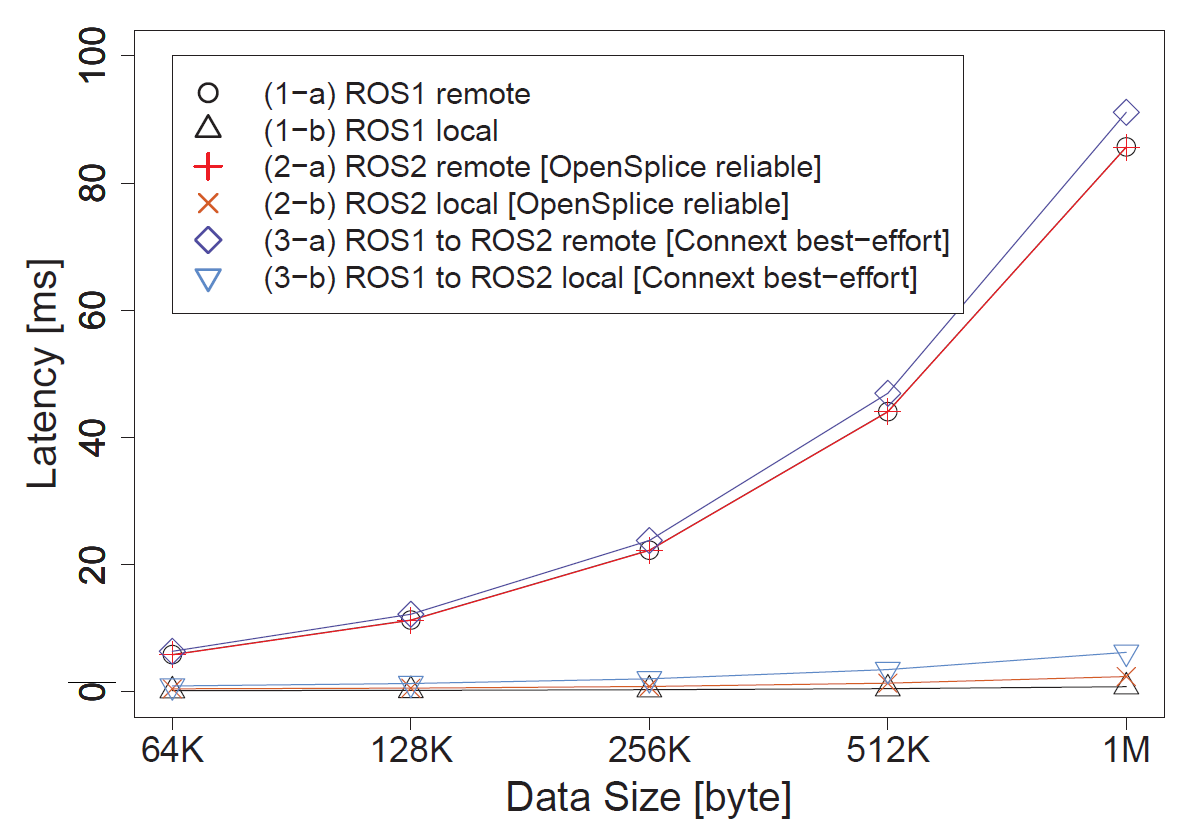
\includegraphics[width=\textwidth]{Bilder/PerformEndtoEnd.PNG}
	\caption{Latency in ROS1 and ROS2 in $[ms]$ for remote/local data transmission of 64 Kbyte to 1 Mbyte by \cite{ROSDDS}.}
	\label{fig_ROS1vsROS2}
\end{subfigure}
\hfill
\begin{subfigure}[b]{0.49\textwidth}
	\centering
	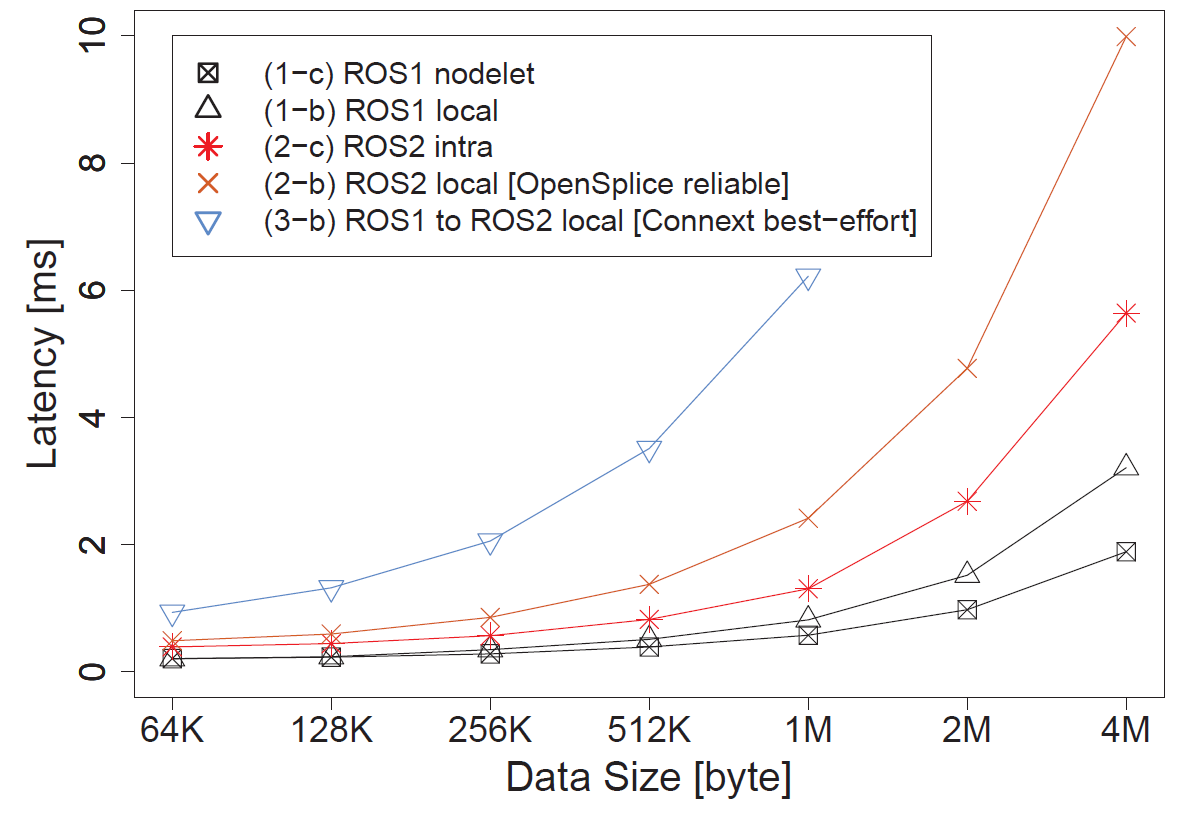
\includegraphics[width=\textwidth]{Bilder/PerformIntra.PNG}
	\caption{Latency in ROS1 and ROS2 in $[ms]$ for local data transmission of 64 Kbyte to 4 Mbyte by \cite{ROSDDS}.}
	\label{fig_ROS1vsROS2Intra}
\end{subfigure}
	\begin{subfigure}[b]{0.49\textwidth}
		\centering
		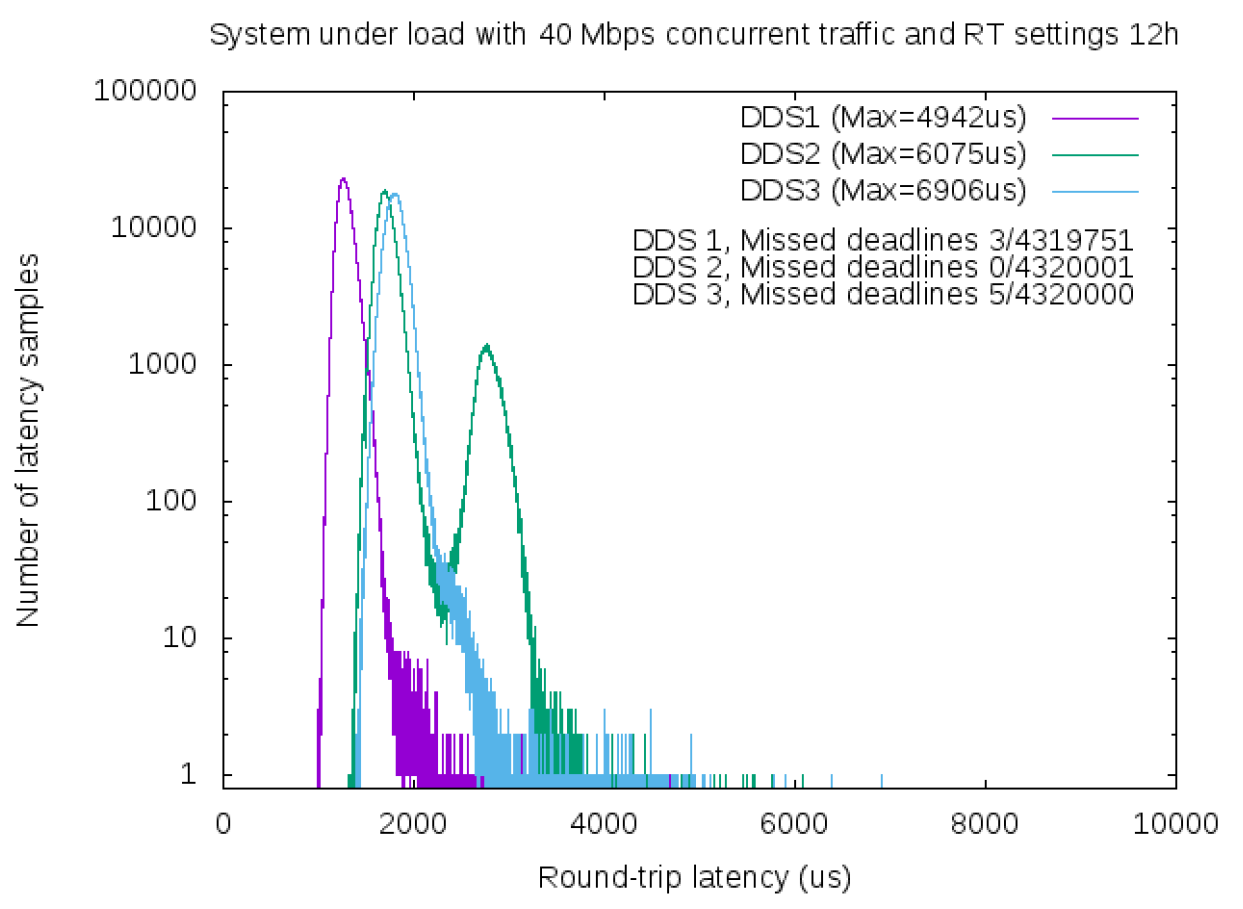
\includegraphics[width=\textwidth]{Bilder/ROS2Realtime.PNG}
		\caption{ROS2 round-trip latency in $[\mu s]$ for three different timing deadlines for 40Mbps in 12h under \ac{CPU} load by \cite{ROSRealtime}.}
		\label{fig_ROS2RT}
	\end{subfigure}
	\hfill
	\begin{subfigure}[b]{0.49\textwidth}
		\centering
		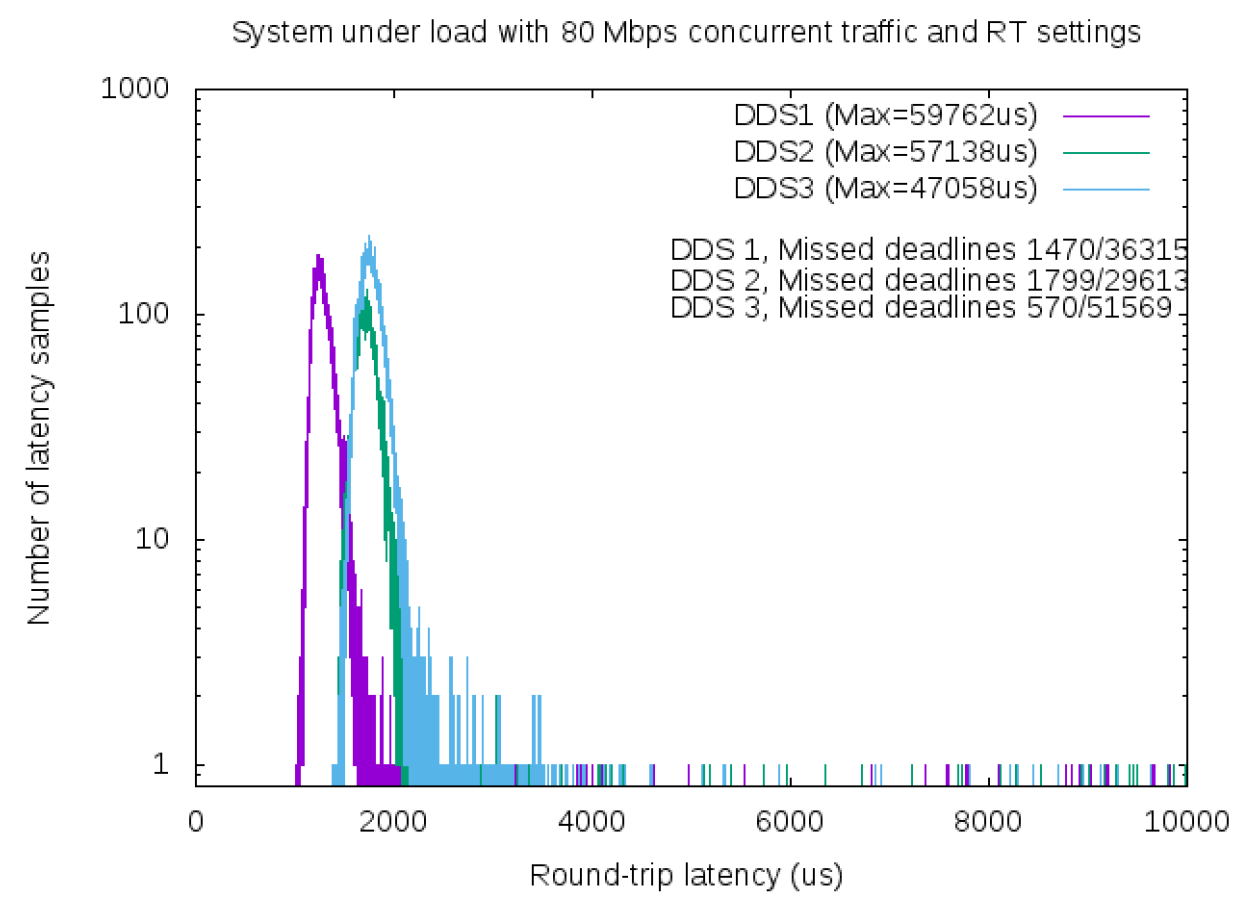
\includegraphics[width=\textwidth]{Bilder/ROS2RealtimeOver.PNG}
		\caption{ROS2 round-trip latency in $[\mu s]$ for three different timing deadlines for 80Mbps in 10min under \ac{CPU} load by \cite{ROSRealtime}.}
		\label{fig_ROS2RTOver}
	\end{subfigure}	
%	\begin{subfigure}[b]{0.49\textwidth}
%		\centering
%		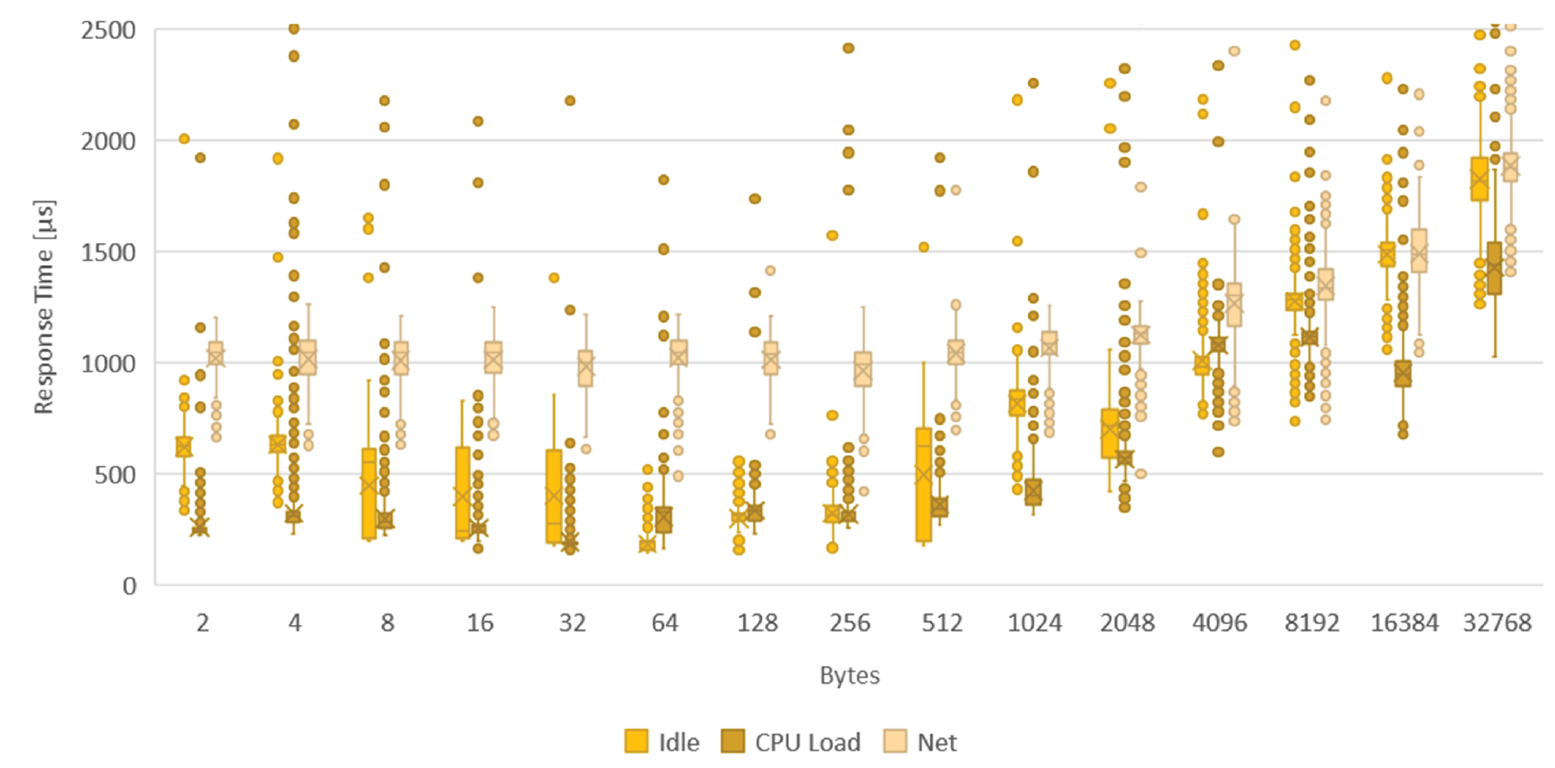
\includegraphics[width=\textwidth]{Bilder/ROS1Perform.PNG}
%		\caption{Echo \ac{RTT} in $[\mu s]$ of data messages in \ac{ROS} from 2 bytes to 32 kbytes by \cite{ROSPerform}.}
%		\label{fig_ROS1Perform}
%	\end{subfigure}
%	\hfill
%	\begin{subfigure}[b]{0.49\textwidth}
%		\centering
%		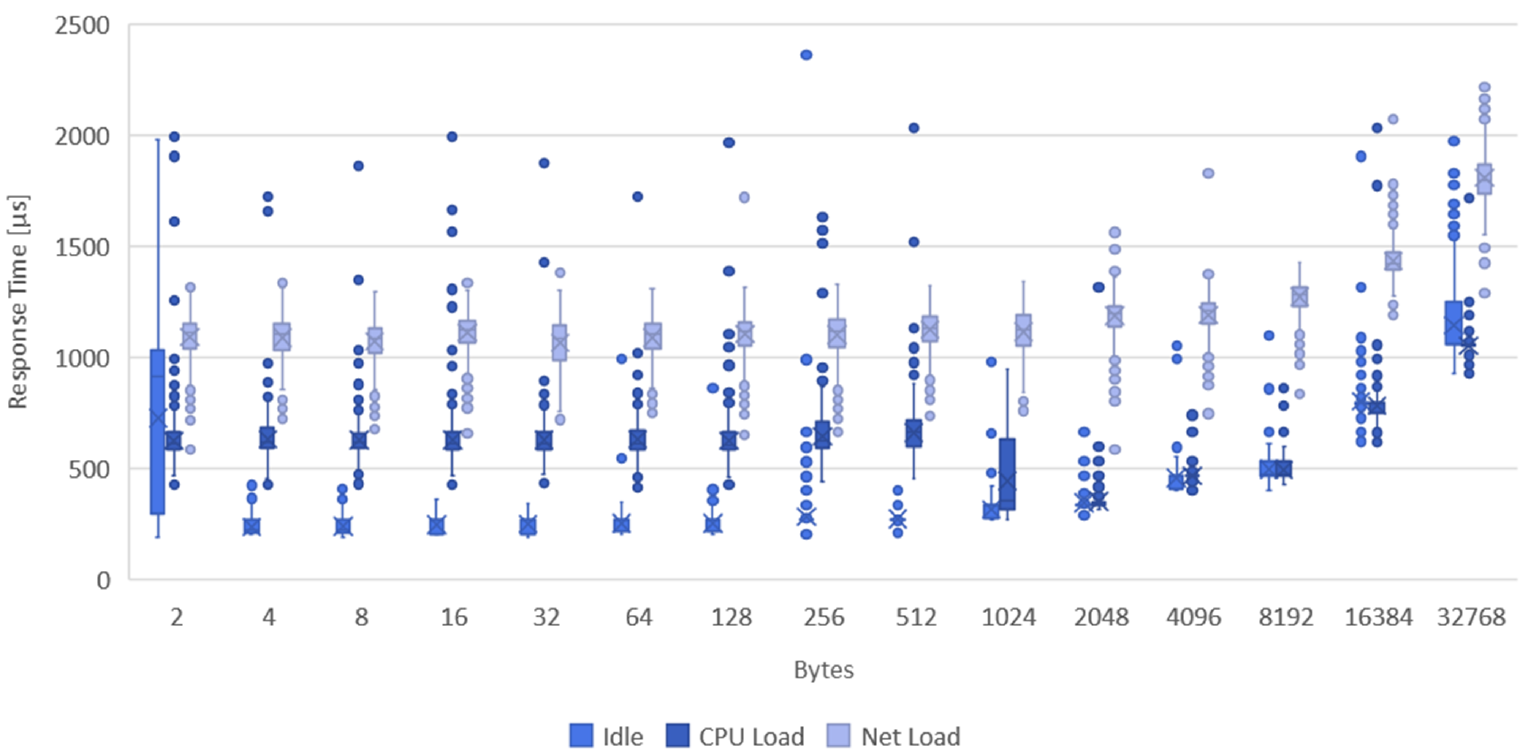
\includegraphics[width=\textwidth]{Bilder/DDSPerform.PNG}
%		\caption{Echo \ac{RTT} in $[\mu s]$ of data messages with \ac{DDS} from 2 bytes to 32 Kbytes by \cite{ROSPerform}.}
%		\label{fig_DDSPerform}
%	\end{subfigure}	
	\caption{ROS data transmission performance.}
	\label{fig_ROSPerform}
\end{figure}
\subsection{Virtual Environment} \label{virtuenv}
Virtual environments has been long used in the development of robotics to test new concepts, strategies and algorithms \cite{Gazebo}. With the inherent limitations of a real world testing environment such as unpredictable weather phenomena, wind induced currents and wakes and time dependent changes of light, simulated environments can increase the availability of suitable test variables, to name one advantage. There are many software solutions to simulate environments, however, especially in the field of \ac{USV}, using the simulation software Unity3D is a viable choice and can be preferred to other simulation software \cite{UnityUSV}. Unity3D is a game engine developed by Unity Technologies and allows for easy development of interactive scenes with a high visual fidelity. An asset store in which a large community  publish textures, models and extensions and other types of predefined assets makes the development process of a new scene efficient. Compared to most other simulation environments, the elements of the virtual environment built with Unity3D are close to the actual environment with an example given by an available high fidelity virtual water surface environment. Furthermore, virtual sensors can be modelled and embedded into the scene through scripts \cite{UnityUSV}. Unity features a powerful PhysX physics engine, a render engine and collision detection engine among others. Of special interest is that there is available a library called \textit{rosbridgelib} for Unity, that links the architectures of \ac{ROS} and Unity by using a \ac{JSON} data format to exchange messages \cite{ROStoUnity}. It has to be noted that this library is officially only implemented for ROS1 and planned only in 2022 for ROS2 as of information in 2021. However, as the message exchange format between ROS1 and ROS2 only differs in specific use cases, the library can as well be used for ROS2.

\section{Module Design}\label{ModuleDes}
% Describe the packages and messages used in ROS and the designstructure in Unity.

\begin{figure}[h]
	\centering
	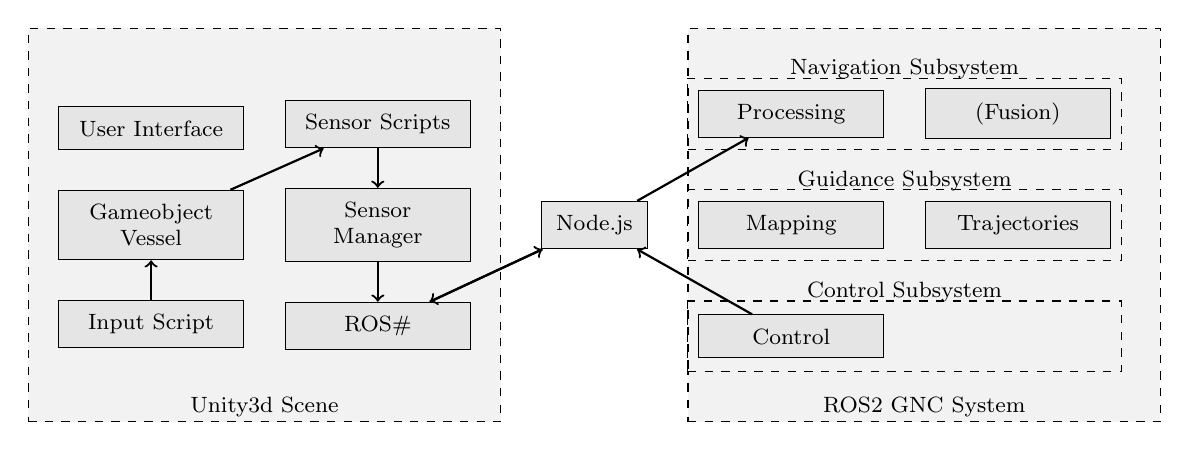
\begin{tikzpicture}
	[node distance = 1cm, auto,font=\footnotesize,
	% STYLES
	every node/.style={node distance=3cm},
	% The comment style is used to describe the characteristics of each force
	comment/.style={rectangle, inner sep= 5pt, text width=4cm, node distance=0.25cm},
	% The force style is used to draw the forces' name
	force/.style={rectangle, draw, fill=black!10, inner sep=5pt, text width=2cm, text badly centered}]
	
	\node [rectangle, draw, fill=black!10, inner sep=5pt, text width=1cm, text badly centered] (Node) {Node.js};
	
	% Box Unity3d with comment
	\node [rectangle, left= 0.5cm of Node, draw, fill=black!5, minimum height=5cm, minimum width=6cm, dashed ] (Unity3d)         {};
	\node [comment, below=-0.5 of Unity3d, text centered]                                 (comment-Unity3d) {Unity3d Scene};
	
	% Boxes right inside Unity3d Scene
	\node [force, right=-2.75cm of Unity3d] (Manager) {Sensor Manager};
	\node [force, above = 0.5cm of Manager] (Sensor)  {Sensor Scripts};
	\node [force, below = 0.5cm of Manager] (ROS)     {ROS\#};
	
	% Boxes left inside Unity3d Scene
	\node [force, left=-2.75 cm of Unity3d] (Vessel) {Gameobject Vessel};
	\node [force, above = 0.5cm of Vessel]  (UI)     {User Interface};
	\node [force, below = 0.5cm of Vessel]  (Input)  {Input Script};
	
	% Links in Unity3d box
	\path[->,thick]

	(Vessel) edge (Sensor)
	(Input) edge (Vessel)
	(Sensor) edge (Manager)
	(Manager) edge (ROS);
	
	
	% ROS2 box with comment
	\node [rectangle, right=0.5cm of Node, draw, fill=black!5, minimum height=5cm, minimum width=6cm, dashed ] (ROS2){};
	\node [comment, below=-0.5 of ROS2, text centered]  (comment-ROS2) {ROS2 GNC System};
	
	% Guidance box with comment
	\node [rectangle, right=0.5cm of Node, draw, fill=black!5, minimum height=0.9cm, minimum width=5.5cm, dashed ] (Guid){};
	\node [comment, above=-0.2 of Guid, text centered]  (comment-Guid) {Guidance Subsystem};
	
	% Navigation box with comment
	\node [rectangle, above =0.5cm of Guid, draw, fill=black!5, minimum height=0.9cm, minimum width=5.5cm, dashed ] (Navi){};
	\node [comment, above=-0.2 of Navi, text centered]  (comment-Navi) {Navigation Subsystem};
	
	% Control box with comment
	\node [rectangle, below =0.5cm of Guid, draw, fill=black!5, minimum height=0.9cm, minimum width=5.5cm, dashed ] (Control){};
	\node [comment, above=-0.2 of Control, text centered] (comment-Control) {Control Subsystem};
	
	% Boxes inside Navigation, Guidance, Control
	\node [force, left=-2.5 cm of Navi]    (Process) {Processing};
	\node [force, right=-2.5 cm of Navi]   (Fusion)  {(Fusion)};
	
	\node [force, left=-2.5 cm of Guid]    (Map) 	 {Mapping};
	\node [force, right=-2.5 cm of Guid]   (Traject) {Trajectories};
	
	\node [force, left=-2.5 cm of Control] (Control) {Control};
	
	% Links to node.js
	\path[->,thick]
	(ROS) edge (Node)
	(Node) edge (Process)
	(Control) edge (Node)
	(Node) edge (ROS);	
	
	\end{tikzpicture} 
	\caption{Modules of the proposed system}
	\label{fig_modules}
\end{figure}

With the tools set according to the requirements, the module design takes place as depicted in figure \ref{fig_modules}. With a focus on the virtual environment, physical sensors are left out of the figure but can as well be integrated in conjunction with or in place of the virtual sensors. Figure \ref{fig_modules} is divided into two main components that are connected with the \ac{ROS} webbridge which is implemented in Node.js. Node.js is an asynchronous event-driven JavaScript runtime environment with the purpose of building scalable network applications. The Unity3d Scene to the left of the Node.js component is composed of a User Interface with which preferences to the Unity Scene such as the screen resolution can be chosen. An input script enables the user to send steering information via keyboard to the virtual vessel which is a Unity3d Gameobject and thus the position of the vessel can be manipulated. Assigned to the vessel are the scripts that simulate the sensors. The scripts send its data to a central Sensor Manager where the data structures are defined with which the data of the sensors can be send with the ROS\# to the \ac{ROS} webbridge. With the introduction of a Sensor Manager, sensors of different types can be easily integrated into the scene and its data types manipulated without changing definitions at various places inside the Unity3d Scene editor.\\ 

With the virtual environment set, the ROS2 component right to the Node.js component is required to receive the sensor data and manipulate it. This is done in three main categories of functions that are set up according the the specification of a \ac{GNC} system. First the Navigation Subsystem processes the received data. As the sensor data, particularly when transmitted combined, can amount to a high data rate, it is advantageous to process them directly in the procedure that receives the data.
After processing the data by filtering, feature extraction and clustering, the results of the different procedures can be fused into a fault resistant representation of the scene. With this representation, the Guidance Subsystem creates a map and calculates trajectories. The points prescribed by the trajectory are then used by the Control Subsystem to generate steering information either for a physical or a virtual implementation of the vessel. As required, the results of the processes inside the categories have to be visualized to the user, so that decisions of the system are understandable.


  \section{Module Implementation}\label{ModuleImp}
This section implements the modules that are specified in section \ref{ModuleDes}. In subsection \ref{VirtEnvStat} the scene in the Unity3d game engine is modelled with static elements such as the terrain and objects. This is followed by the design of the dynamic elements that are navigated through the scene e.g. a vessel and different sensors (\ref{VirtEnvDyn}). A third subsection \ref{DataProcessing} details the \ac{ROS} network that is programmed to process the data of the sensors in the Unity3d scene.

\subsection{Static environment} \label{VirtEnvStat}
% The code level, pseudo code in the modules, most detailed description.
In a first step, the virtual scene is modelled in Unity3d running on Linux 20.04 LTS. As a geographic reference for the terrain, the location proposed for the physical implementation of the project \ac{ELLA} is used. Elevation data for this location in the reference coordinate system EPSG 25832 for the position and EPSG 7837 for the height from east 384999 to west 383000 and from north 5720999 to south 5719000 is provided in .xyz data by OpenDataNRW with a resolution of one meter \cite{Xyzdata}.\\

The data is loaded into to the software QGIS Version 3.16.6 LTR. QGIS is an open source geographic information system and provides various functionalities in this domain. One of them is the creation of a \ac{TIN} which can represent a \ac{DEM}. Given a function $z = f(x,y)$ in which $x$ and $y$ represent the position data and z the according height, the function can be computed only for discrete points as $x$ and $y$ are finite in $S$ and depend on the resolution of the source. Therefore, in order to map the \ac{DEM} continuously, a \ac{TIN} has to be created that connects the discrete points so that they suffice three conditions. First the number of vertices $T$ of the resulting triangles have to be equal to the number of points $S$. As a second condition the interiors of the triangles out of $T$ are not allowed to intersect each other and if the boundaries of two triangles intersect each other, the intersection has to be either a common edge or a common vertices. On the resulting triangles, a linear interpolation function can be applied and thus a continuous \ac{DEM} approximation is achieved \cite{TIN}.\\

To convert the \ac{DEM} to a .raw heightmap that is used by Unity3d to create a terrain, the \ac{DEM} is converted to a .TIFF and exported to Gimp. Gimp is an open source image manipulation program and supports various file formats of which the .raw format is one. The resulting image is shown in figure \ref{fig_HenrichHeight}. On a 256-bit greyscale resolution the darker regions of the image represent low terrain with increasing height for every step towards white. With the import function of Unity3d the terrain is then shaped according to the heightmap. The resulting terrain data is visualized in figure \ref{fig_terrainRaw}. The sink in the bottom-left of the image matches the second dark shape along the top of figure \ref{fig_HenrichHeight}.\\ 
\begin{figure}[!htb]
	\begin{minipage}[t]{0.48\textwidth}
		\centering
		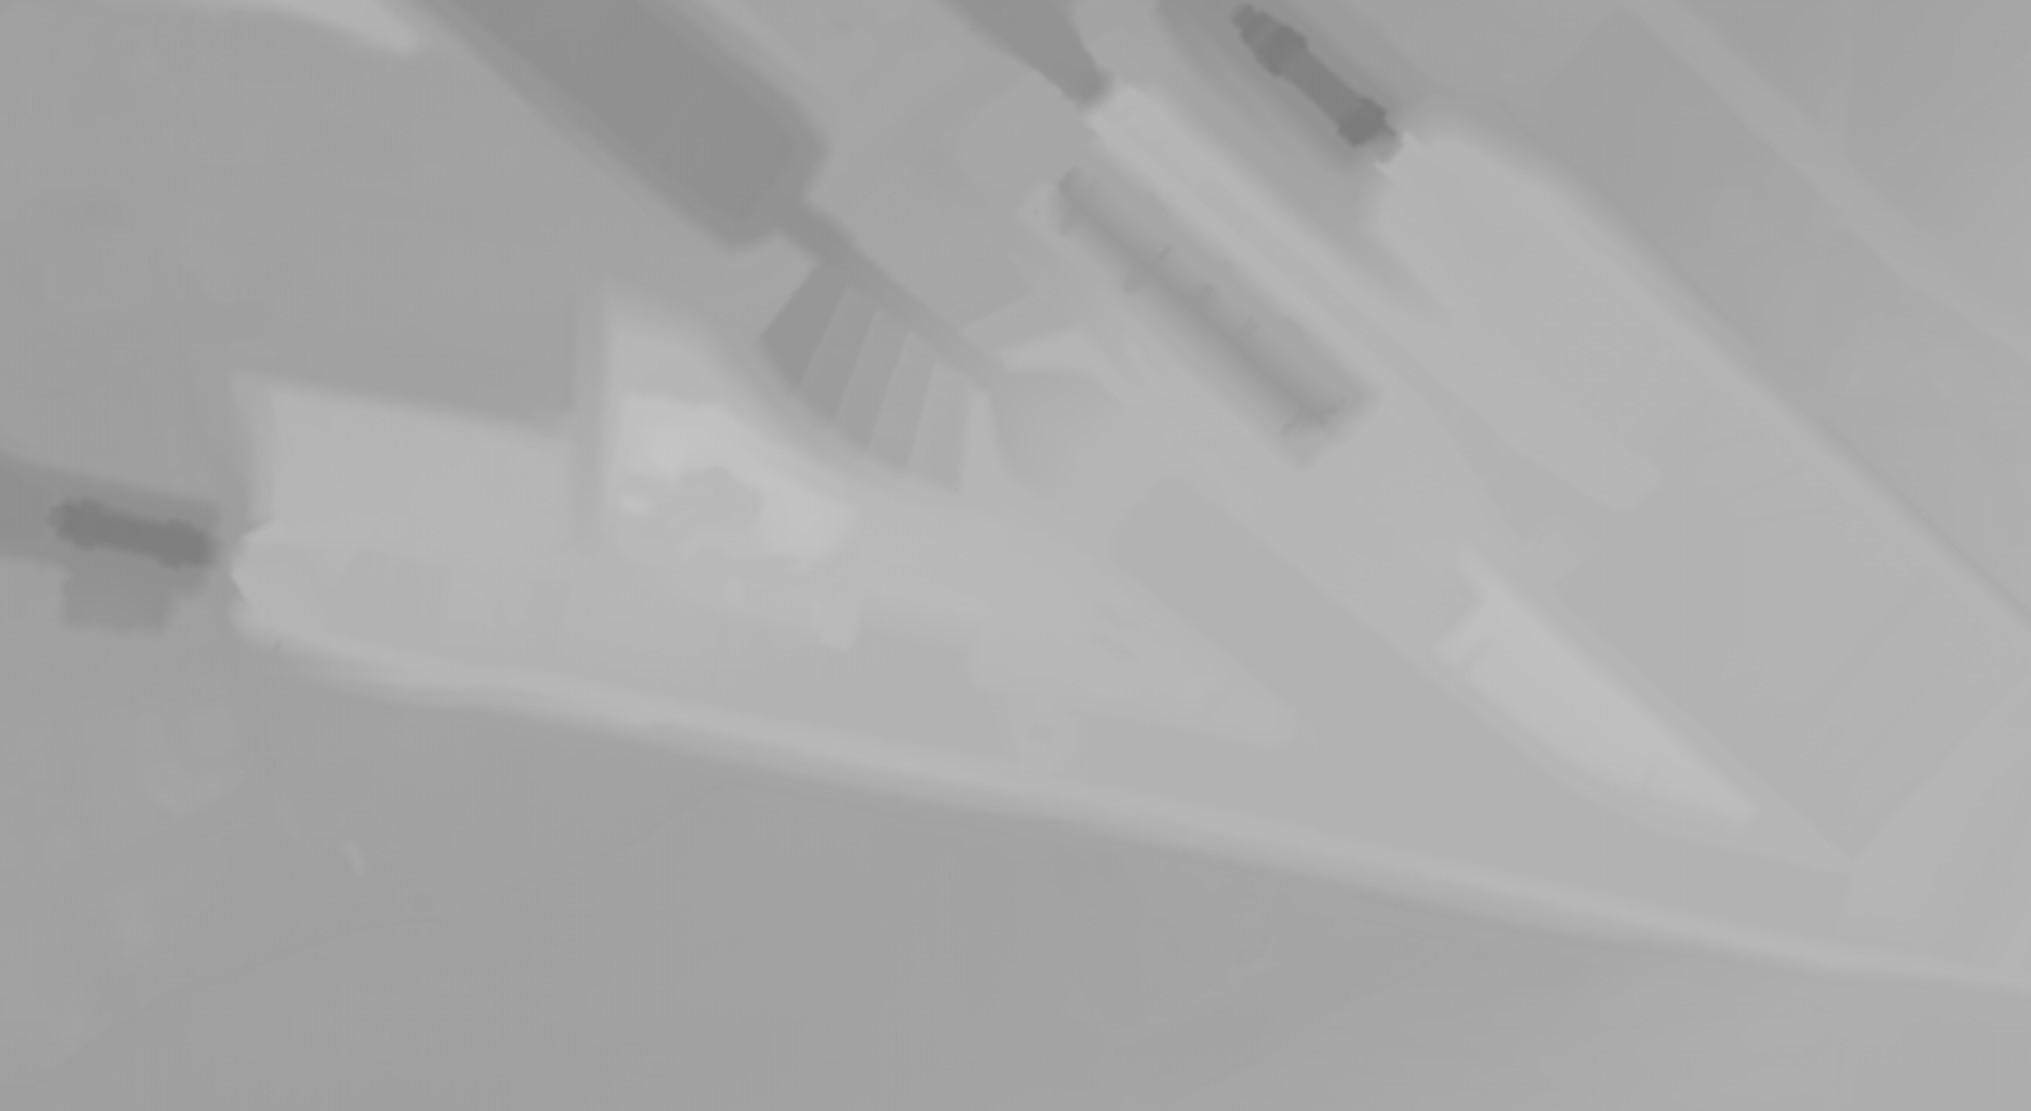
\includegraphics[width=.99\linewidth]{Bilder/Henrich_SE.jpeg}
		\caption{Height map of the scene that is to be modelled}\label{fig_HenrichHeight}
	\end{minipage}\hfill
	\begin{minipage}[t]{0.48\textwidth}
		\centering
		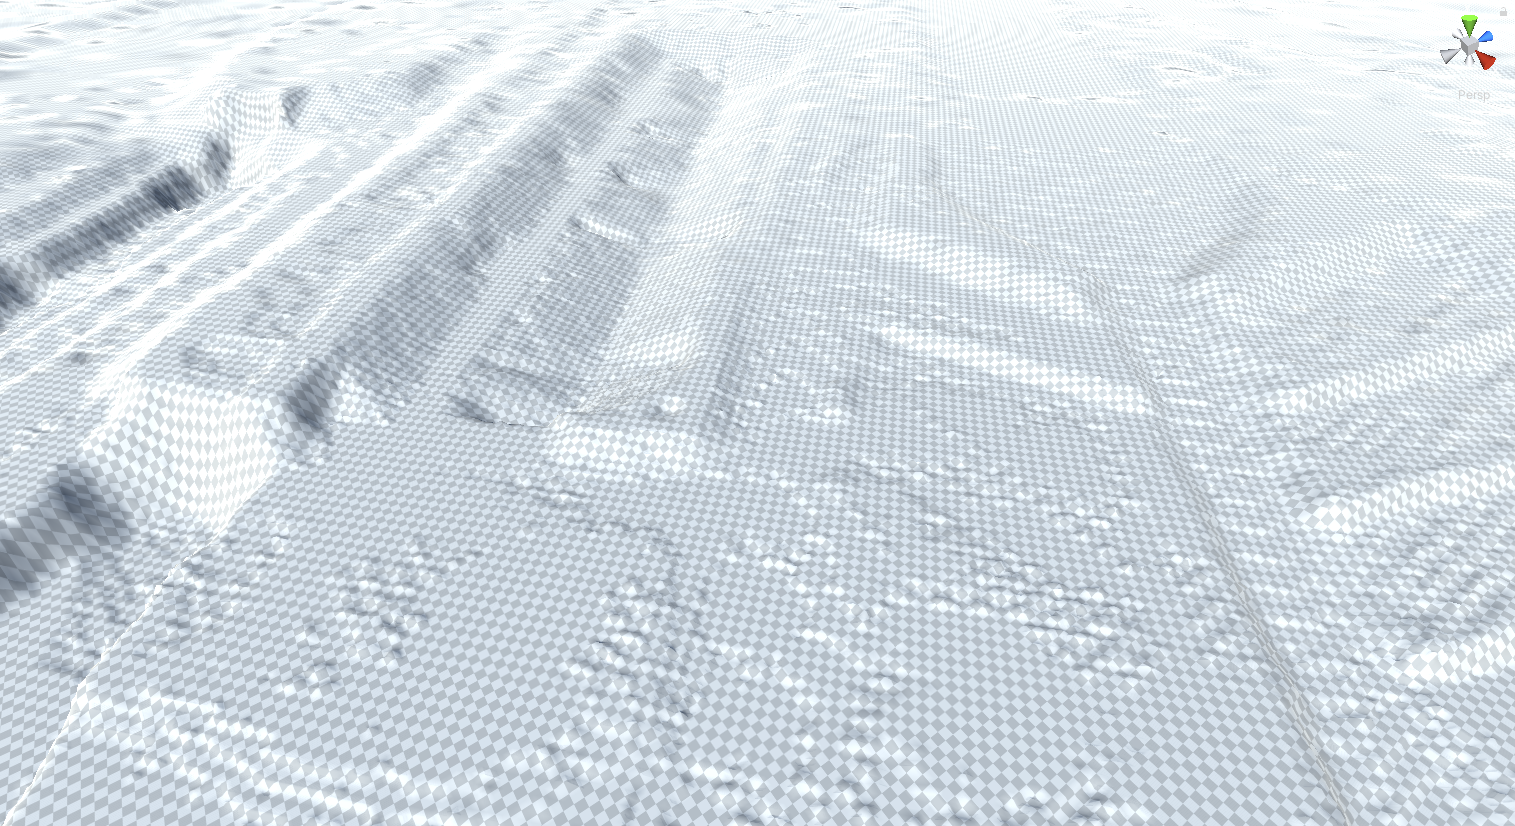
\includegraphics[width=.99\linewidth]{Bilder/terrainRaw.png}
		\caption{Terrain data in Unity3d derived from a height map}\label{fig_terrainRaw}
	\end{minipage}
\end{figure}

Another option to create a terrain out of the \ac{DEM} is represented by importing the data into blender and create a mesh that is then exported to Unity3d as an object. However it turned out that the advantage that comes with the possibility of granular mesh manipulation is at the same time a disadvantage. A highly intersected mesh with a very large amount of vertices can not be easily joined without destroying the integrity of the mesh, that is the consistency of vertices connections. Thus the larger the area that is modelled and the more details in terms of position resolution is required, the less manageable the mesh becomes in terms of processing time required for visualization.\\

The terrain as shown in figure \ref{fig_terrainRaw} is smoothed which is necessary because of the limited resolution of the height map that is restricted to 256-bit on the greyscale that represents the height. On the resulting terrain, a satellite image of the scene serves as a background texture. Various other textures are then applied to the scene to resemble the real environment. In the software Blender 2.92.0, 3D objects are created and imported into the virtual environment. As the process of creating the objects and applying textures and shader as well as collision meshes to the objects is rather tedious, only objects that are vital to the scene are modelled. For reasons of simplicity only rigid bodies are used in the scene. Rigid bodies are volume bodies in which every set of two different arbitrary points contained in the body have the same distance to each other at any time. Figure \ref{fig_smallvessel} shows the Blender model of the small vessel that is used in the Unity3d scene. It is composed of multiple connected objects that can be used to derive a collision mesh from. The collision mesh surrounding the vessel inside the modelled scene is depicted in figure \ref{fig_collisionmesh} with the mesh coloured in green. There are two option for the generation of the mesh in Unity3d. A concave mesh takes the vertices inside the object and a convex mesh is laid over the vertices outside. The collision mesh as depicted is a convex shape. It can be noted that there are differences of the mesh to the shape of the visible object that results of the inability of the mesh to project on concave and convex parts in the same object.\\

 	\begin{figure}[!htb]
 	\begin{minipage}[t]{0.48\textwidth}
 		\centering
 		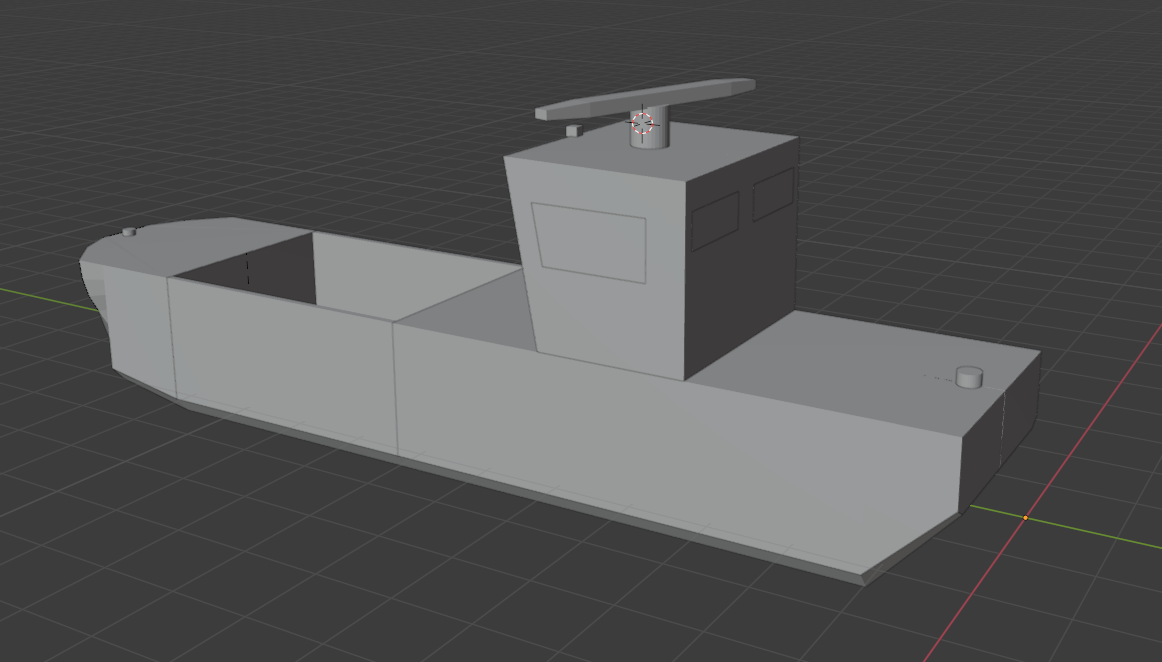
\includegraphics[width=.99\linewidth]{Bilder/BlenderVessel.png}
 		\caption{Blender vector model of a small vessel used in the modelled scene}\label{fig_smallvessel}
 	\end{minipage}\hfill
 	\begin{minipage}[t]{0.48\textwidth}
 		\centering
 		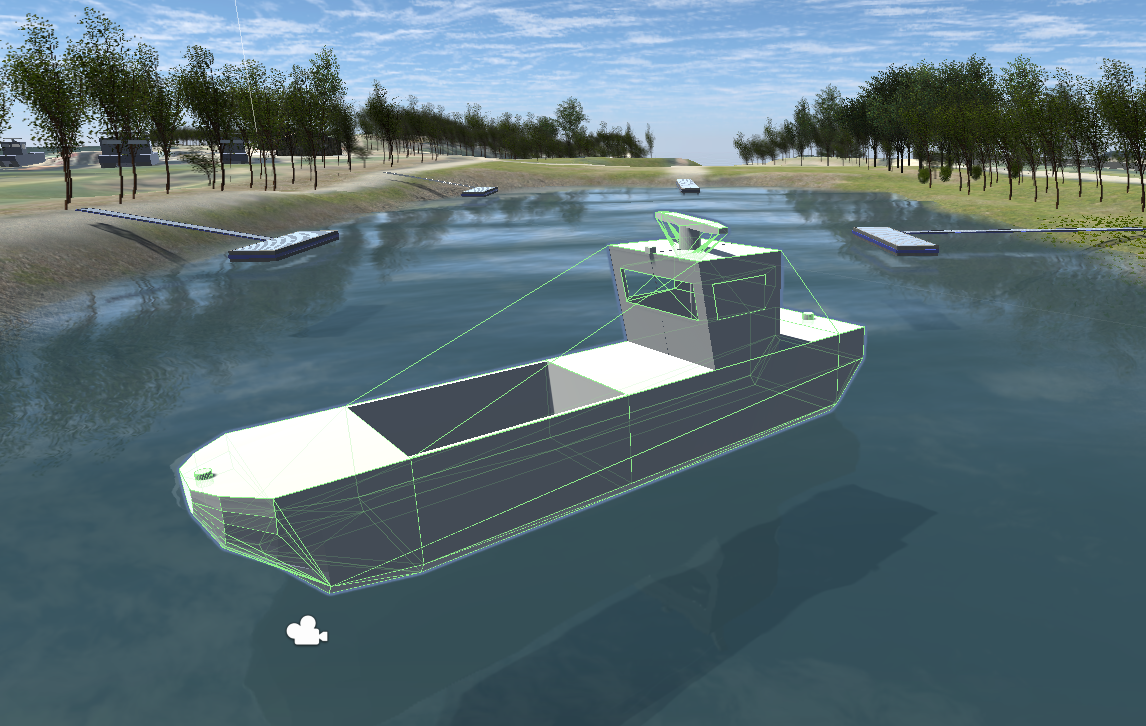
\includegraphics[width=.99\linewidth]{Bilder/CollisionmeshVessel.png}
 		\caption{Small vessel with collision mesh generated from the blender model}\label{fig_collisionmesh}
 	\end{minipage}
 \end{figure}

The scene as seen from above is shown in figure \ref{fig_UnityBird}. The V-shaped river is in the center of the image with a total of five landing stages and two small vessel located on it. With a satellite image as a background, texures for paths, meadows and the rivers shore are applied on the terrain. Trees and houses further detail the scene. The water is represented by a mesh of Unity3d's standard assets. The standalone application that can be run without a Unity3d IDE can be seen in figure \ref{fig_UnityPerson}. Settings in the top left of the application allows for the change of perspective out of which the scene is rendered, the change of resolution and for reloading or closing the scene. In the foreground the small vessel on which the sensors are mounted can be seen. In the background, the aforementioned textures and objects are visible.
 \begin{figure}[!htb]
 	\begin{minipage}[t]{0.48\textwidth}
 		\centering
 		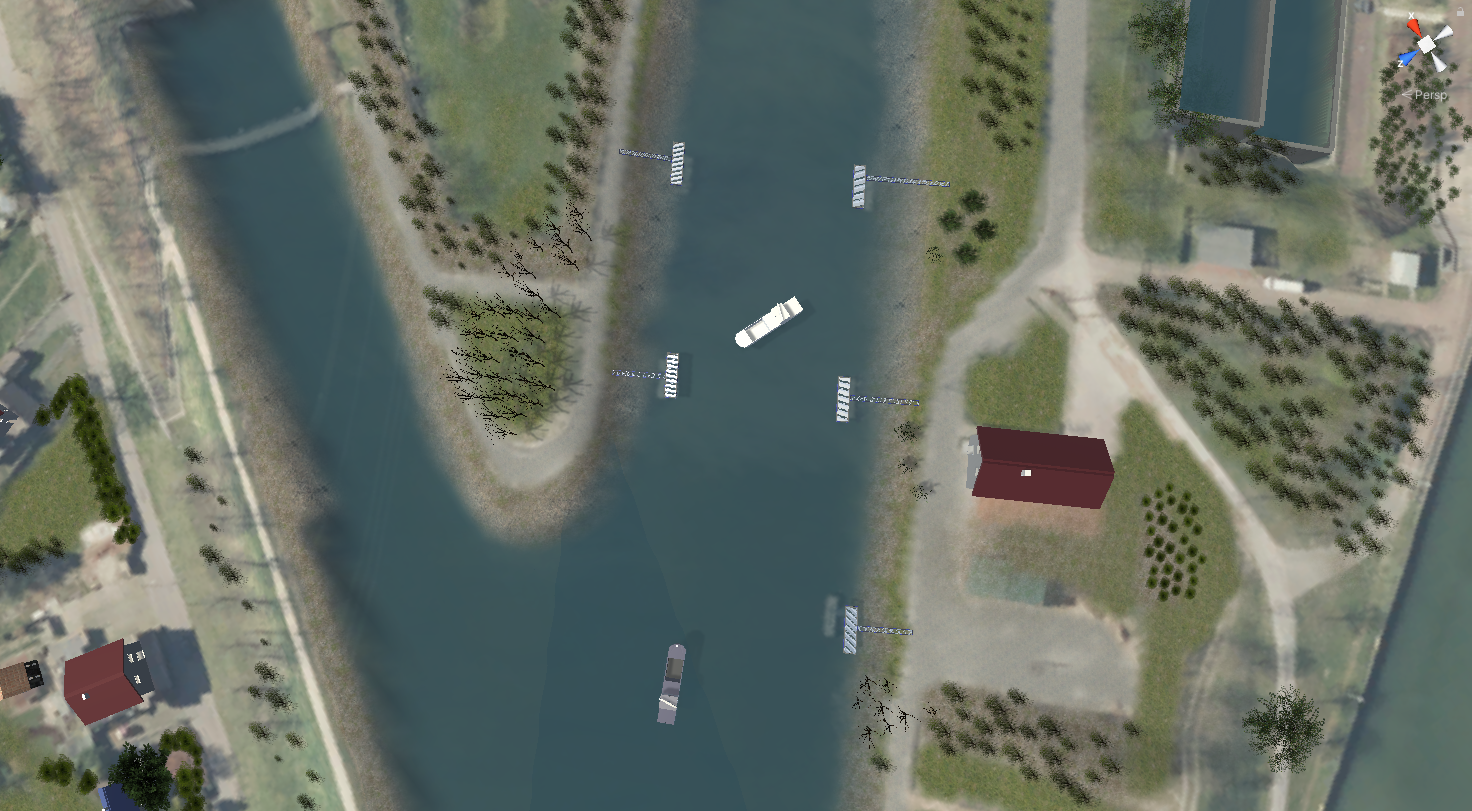
\includegraphics[width=.99\linewidth]{Bilder/UnitySceneBird.png}
 		\caption{Unity3d scene from above}\label{fig_UnityBird}
 	\end{minipage}\hfill
 	\begin{minipage}[t]{0.48\textwidth}
 		\centering
 		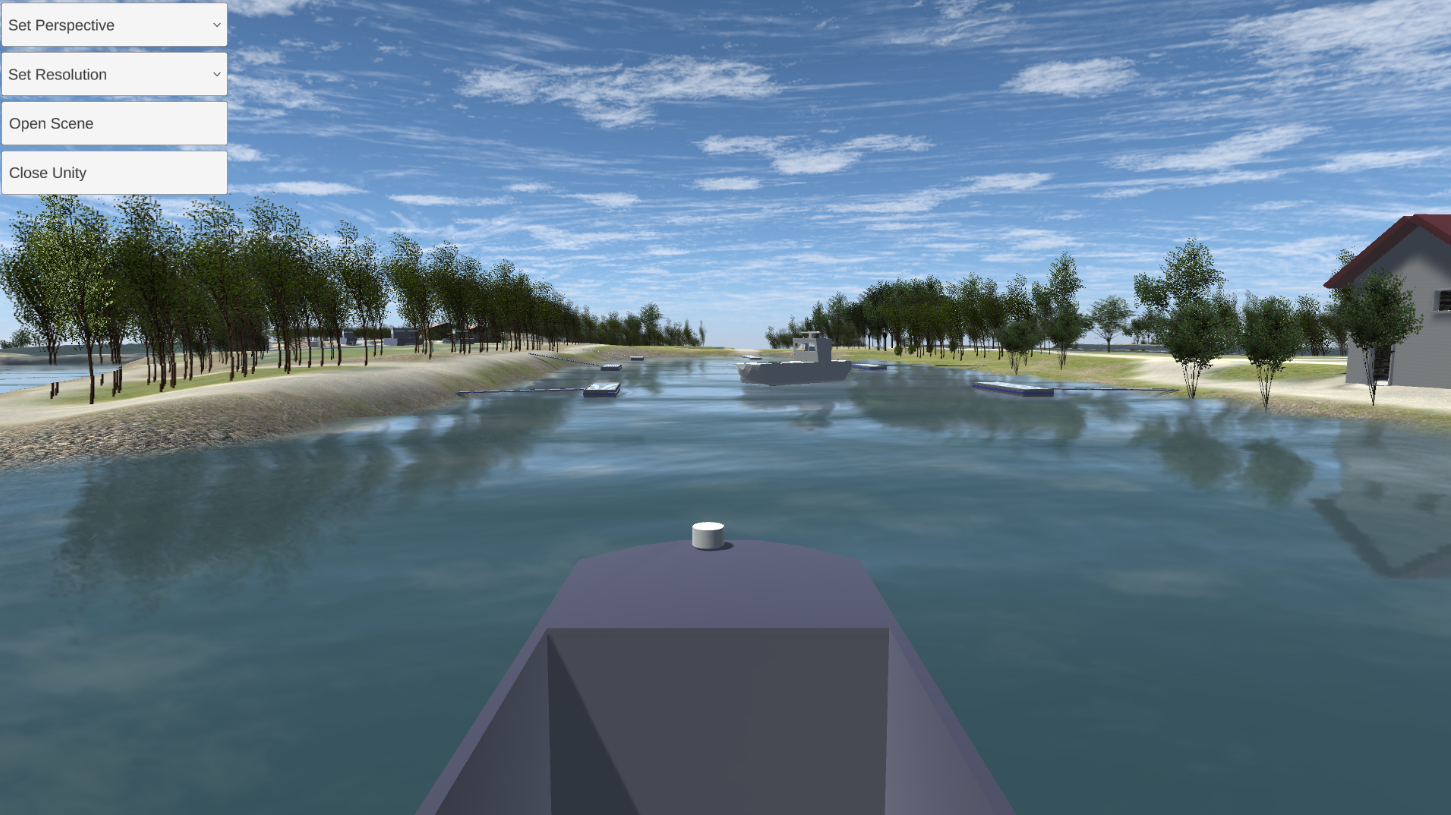
\includegraphics[width=.99\linewidth]{Bilder/UnitySceneFirstPerson.png}
 		\caption{Unity3d with menu from sensor perspective}\label{fig_UnityPerson}
 	\end{minipage}
 \end{figure}



\subsection{Dynamic Environment} \label{VirtEnvDyn}

With the scene modelled, defining its behaviour during runtime is the next step. To obtain a realistic physics simulation, Unity3d makes use of a physics engine. The main task of a physics engine is to solve forward dynamics, however there are many factors that determine the performance of a physics engine and thus there are many different implementations available. Collision and energy restitution, the modelling of constraints and the integrator performance are among the factors that can be evaluated in order to determine a suitable implementation. Unity3d default physics engines are PhysX supplied by Nvidia and Havok Physics supplied by Havok. It has to be noted, that both engines are optimized towards the appliance in games and therefore a strong focus is on the engines stability rather then the accuracy \cite{PhysXComp}. In Unity3d, the physics module provides an abstraction level to access functions related to 3D physics. These functions are used among others to steer a small vessel with a keyboard input through the scene. The forward movement and the rotation of the vessel are taken as an input and serve the purpose of altering the position of the virtual sensors that are mounted on the vessel.\\

All data types of the sensors are saved in a central script called Sensor Manager. For every sensor instance, a public data storage class is instantiated that can be accessed by the sensor class as well as by the class that sends the data to the \ac{ROS} network. The foundation of what is used as a \ac{LIDAR} sensor and \ac{IMU} sensor in Unity3d is already defined. Only the saving process is changed to allow an adaptation to the outlined data exchange method. The \ac{LIDAR} sensor class makes use of the so called raycast, which is one method provided by the physics engine to provide scene queries. A point cloud in the scenes global coordinate system results of the colliders that are hit by the emitted rays. Various variables such as the field of view and the sweep frequency allow for the simulation of physical implemented sensors. To transmit the pointcloud, its three-dimensional cartesian positional data is saved with one list for each dimension. A list with an altering size for each cycle comes with the disadvantage of a required memory allocation for every measurement cycle. However, as the data size of the pointcloud is changing depending on the objects that are hit by the raycast, a list allows for having the lowest data size possible.\\

Based on the physical operating principle of a real \ac{RADAR}, a virtual \ac{RADAR} is implemented in Unity3d as depicted in figure \ref{fig_radarrays}. The emittance of an electromagnetic wave of a real \ac{RADAR} is simulated by a discrete beam that consists of raycasts. As a sequential calculation of the collisions of objects with the emitted rays increases the process time and decreases the simulation performance, a job handle is used that is implemented in the \ac{LIDAR} sensor as well. A job handle allows for parallel execution of tasks and thus can increase the process time. The resolution of the discrete beams is adaptable with a variable in the script of the sensor. Each time an object is hit by the raycast, the positional data is saved together with a reflectance value of the object. The reflectance value is provided by a script that can be attached to objects to further detail its  material properties. That is useful especially for a \ac{RADAR} as the reflected energy not only results of the object size but of the objects material, too. After one turn that consists of a predetermined number of beams, the cartesian three-dimensional positional data of all detected objects is mapped to a two-dimensional space by omitting the height data.\\
\begin{figure}
	\begin{centering}
		\centering
		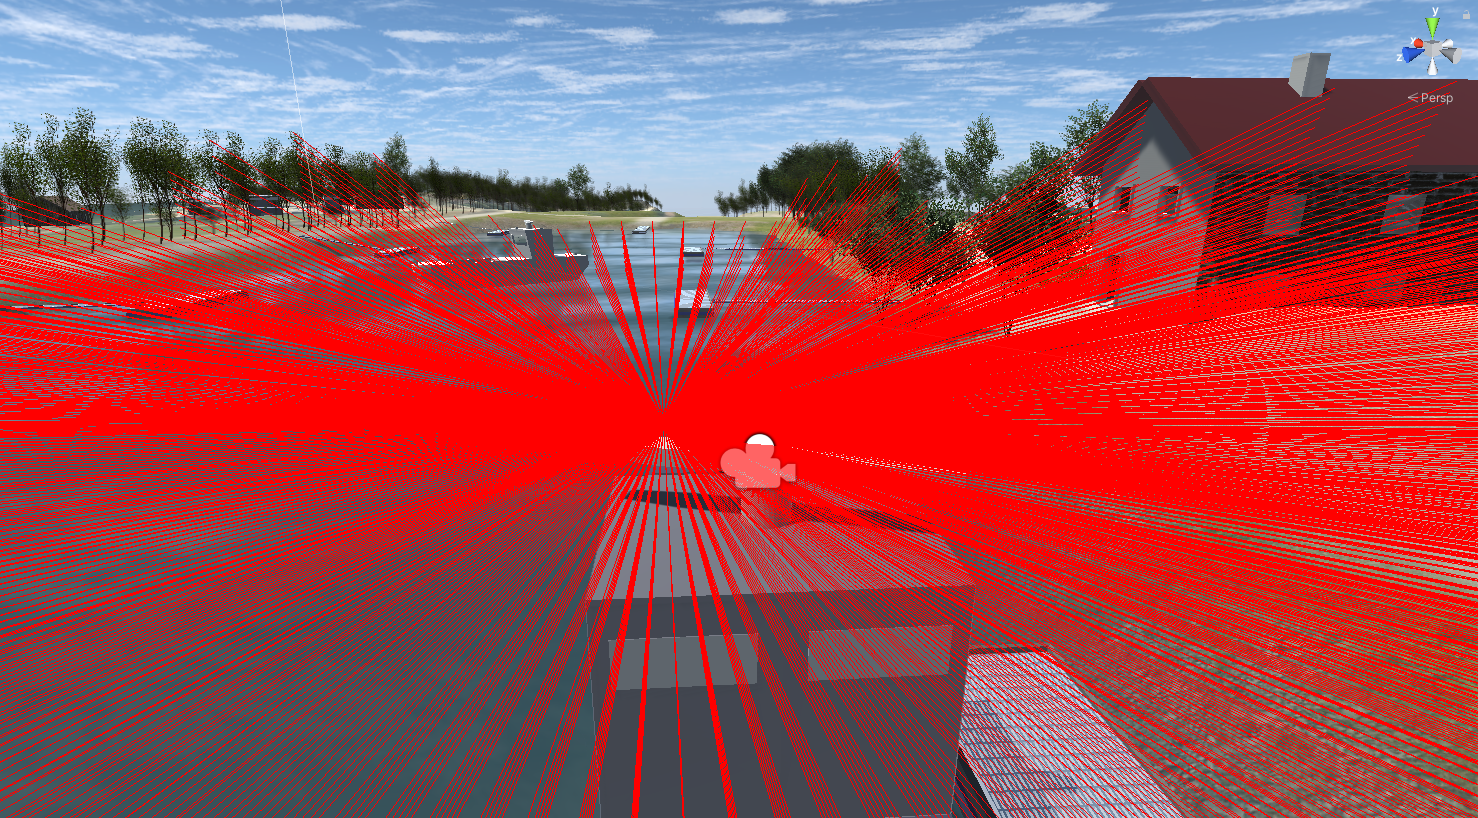
\includegraphics[width=0.6\linewidth]{Bilder/radarrays.png}
		\caption{Raycast of the radar with active rays visualized  in red}
		\label{fig_radarrays}
	\end{centering}
\end{figure}

To resemble the image of a radar, an array  is set up with the length resulting of the predetermined number of beams multiplied by the set cell extension in every beam. Starting at the center $M$ that is the sensor center, the array consists of the subsequent beams cell values. Each cell can be accessed with an index as shown in figure \ref{fig_radarPol} and is defined by its radius $r_{min}$ and $r_{max}$ and angle theta $t_{min}$ and $t_{max}$. The quantity $C$ of points inside the cell now follow equation \ref{eq_insideCell}. 
\begin{equation}
C = {r,t| r_{min}<r>r_{max} \wedge t_{min}<t>t_{max}}
\label{eq_insideCell}
\end{equation}
 The two-dimensional cartesian positional data is transformed to a quantity of polar coordinate representations called $P$. The points $I$ inside the cell now follow equation \ref{eq_PinsideCell}. 
\begin{equation}
	I = P \cap C
\label{eq_PinsideCell}
\end{equation}
The reflectance value $r$ of the each cell can be calculated with equation \ref{eq_RefinsideCell} with $ref_i$ being the aforementioned individual reflectance for each object. Each value can be saved to the array that can then be transmitted to the Sensor Manager.\\
\begin{equation}
% || = how many elements inside the quantity
r = \sum_{i=0}^{i=|I|} I_i * ref_i
\label{eq_RefinsideCell}
\end{equation}


 \begin{figure}
	\begin{centering}
		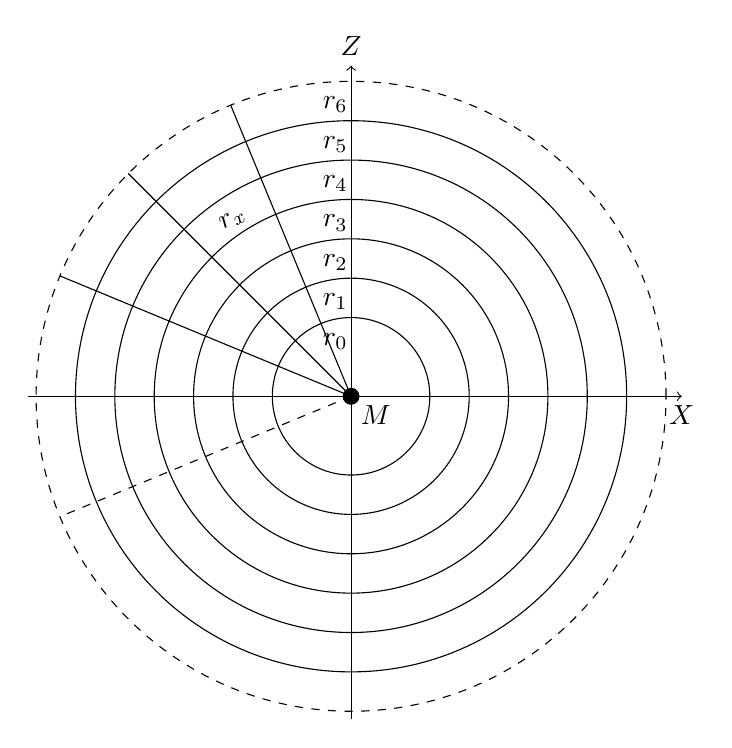
\begin{tikzpicture}      
		%\draw[help lines,xstep=.5,ystep=.5,dashed] (0,0) grid (10,10); %Hilfsdiagramm für Koordinaten
		%\foreach \x in {0,1 ,...,10} { \node [anchor=north] at (\x,0) {\x}; }
		%\foreach \y in {0,1,...,10} { \node [anchor=east] at (0,\y) {\y}; }
		
		\draw[->,] (0.9,5) -- 	(9.2,5) node  [at end,anchor= north]{$X$}; %x axis
		\draw[->,] (5,0.9) -- 	(5,9.2) node  [at end,anchor= south]{$Z$}; %z axis
		
		\draw[fill=black]       (5,5) circle (0.1) node (M)[below right]{$M$}; % point M
		
		\draw      (5,5) circle (1) node (M1){}; % first circle around center
		\draw      (5,5) circle (1.5) node (M2){}; % circle around center
		\draw      (5,5) circle (2) node (M3){}; % circle around center
		\draw      (5,5) circle (2.5) node (M4){}; % circle around center
		\draw      (5,5) circle (3) node (M5){}; % circle around center
		\draw      (5,5) circle (3.5) node (M6){}; % circle around center
		\draw [dashed]     (5,5) circle (4) node (M7){}; % last circle around center
		
		\draw[-,] (5,5) -- 	(3.47,8.7) node  [at end,anchor= north]{}; % 22.5 degree 
		\draw[-,] (5,5) -- 	(2.17,7.83) node  [at end,anchor= north]{}; % 45 degree 
		\draw[-,] (5,5) -- 	(1.3,6.53) node  [at end,anchor= north]{};% 67.5 degree
		\draw[dashed] (5,5) -- 	(1.3,3.47) node  [at end,anchor= north]{};% 115.5 degree
		
		
		\draw[fill=black]       (4.8,5.7) circle (0) node (C)[]{$r_0$}; % point 1
		\draw[fill=black]       (4.8,6.2) circle (0) node (C)[]{$r_1$}; % point 2
		\draw[fill=black]       (4.8,6.7) circle (0) node (C)[]{$r_2$}; % point 3
		\draw[fill=black]       (4.8,7.2) circle (0) node (C)[]{$r_3$}; % point 4
		\draw[fill=black]       (4.8,7.7) circle (0) node (C)[]{$r_4$}; % point 5
		\draw[fill=black]       (4.8,8.2) circle (0) node (C)[]{$r_5$}; % point 6
		\draw[fill=black]       (4.8,8.7) circle (0) node (C)[]{$r_6$}; % point 7
		\draw[fill=black]       (3.5,7.25) circle (0) node (C)[rotate=30]{$r_{x}$}; % point 1
		
		\end{tikzpicture}
		\caption{2D Cartesian and polar coordinates with index and reflectance value of \ac{RADAR} cells.}
		\label{fig_radarPol}
	\end{centering}
\end{figure}

To send sensor data to \ac{ROS}, a library for Unity3d called ROS\# is used. ROS\# can be integrated into Unity3d and makes use of the messages that are defined in \ac{ROS}1. As there are only few differences in the default messages provided by \ac{ROS}1 to the subsequent implementation \ac{ROS}2, the library can be used for both frameworks. However, it is noted that the message of type header makes use of a different notation for time units and thus has to be adjusted. In addition to default messages, \ac{ROS} provides the possibility to define custom messages that can then be exported to ROS\#. Custom messages in the context of the particular use case are derived from the sensor data classes. As a webbridge run by Node.js serves as an intermediary framework for data transmission, new messages types have to be introduced to it as well.\\

\subsection{Data processing} \label{DataProcessing}

New message transmitted to the \ac{ROS} network are first received by the nodes that process the message data. In \ac{ROS} nodes are executables that can communicate to other nodes with an interface such as datatypes defines in messages. To avoid stressing the network with high data rates, for large messages a design maxim in this project is the reduction of data size in the first node that receives the data. That can be done by algorithms that for example filter, cluster and segment data. \\

Figure \ref{fig_rqt} displays the structure of the data processing in \ac{ROS}. The node transform\_listener is not used as it is only relevant for coordinate system transformations that are not taking place in the scope of this work. The ros2\_web\_bridge-node connects to the programmed Unity3d scene and receives its messages. A total of four \ac{ROS} nodes that are named image\_subscriber, lidar1\_xyz, radar1\_img and get\_imu process the incoming data. After being processed, the lidar and radar data are published again and are received by the n\_rviz node that is a predefined \ac{ROS} visualization tool.  \\
\begin{figure}
	\centering
	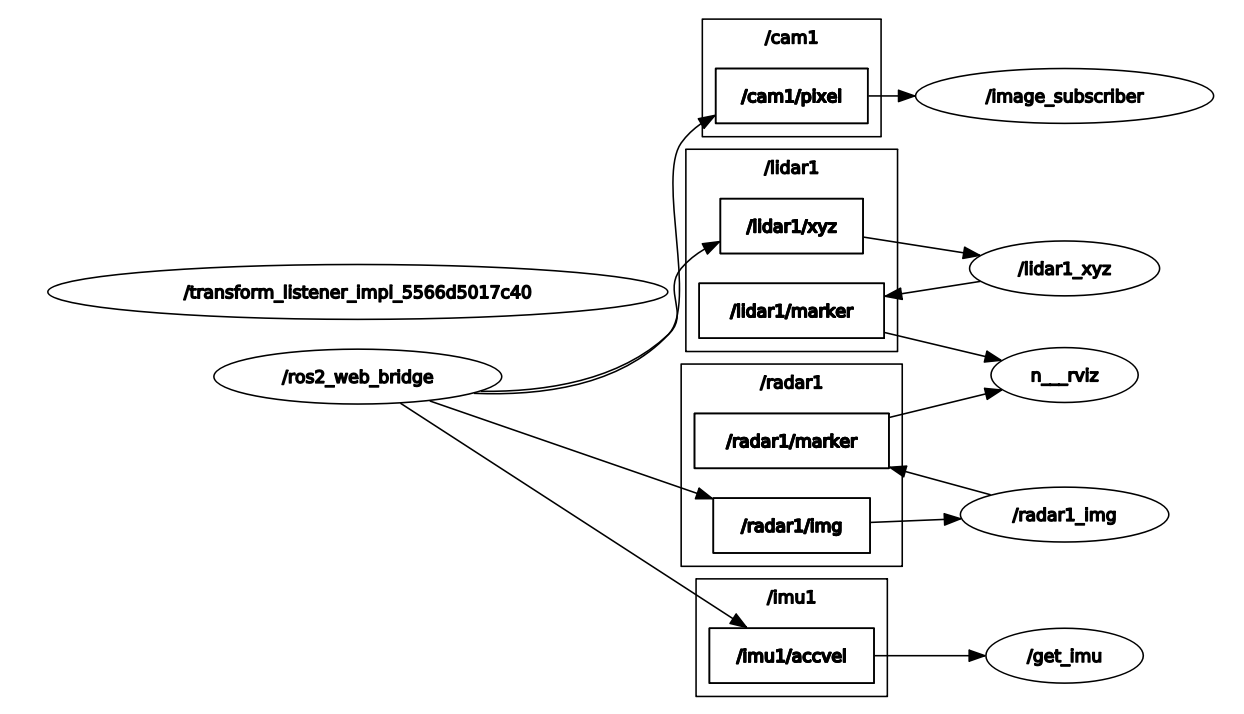
\includegraphics[width=.99\linewidth]{Bilder/rviz2.png}
	\caption{Node and interface structure of ROS2 navigation package}
	\label{fig_rqt}
\end{figure}

The incoming \ac{IMU} data is not further processed but solely displayed as shown in figure \ref{fig_IMU}. The angular velocity in $x$,$y$ and $z$ as well as the acceleration information of the sensor is plotted in a time frame of five seconds. As in Unity3d the sensor is mounted on a object without further specified physical characteristics, the object acceleration in positive as well as negative direction is not further specified by properties such as weight. Presumably this accounts for the rapid changes in for example the acceleration in $x$ direction. The visualization makes use of the \textit{matplotlib} library for python with the plot style set to continuous plotting. It has to be kept in mind that the library as well as \ac{ROS} has its own event handling and resulting loop. Therefore, not every setting of \textit{matplotlib} can be used for plotting data together with \ac{ROS}. \\

The \ac{LIDAR} data that is received from the Unity3d scene has to be processed in order to extract obstacles that are used to map the environment. As there are many algorithms that operate on large datasets of three dimensional data, the approach that is best suited for the application has to be found. The Hough Transform Algorithm directly extract contours in the data it is applied on. That comes in handy as it requires no other processing. However as on every point of the data iterations are conducted, it can be expected that the method does not provide the performance used for realtime applications in which new data comes in at high intervals. The same drawback counts for the disqualification of the partition based K-Means clustering algorithm. Additionally, this algorithm only gets to local optimal solutions in a limited processing time. The hierarchic \ac{BIRCH} clustering algorithm tends to subdivide large cluster that in fact are intended to be viewed as one cluster. The last discussed algorithm is the density based \ac{DBSCAN} clustering algorithm. An advantage of this method is the detection of noise that can then be neglected for mapping the environment. This algorithms promises the best results as no disadvantages can be noticed. Thus it is applied in the node that clusters the \ac{LIDAR} data in an implementation that makes use of parallel procession of points \cite{ParaDBSCAN}. Figure \ref{fig_lidarMat} displays the segmented data. For example the coloured vertical lines can be classified as colliders of trees. Again, \textit{matplotlib} is used for the data visualization.\\
 \begin{figure}[!htb]
 	\begin{minipage}[t]{0.48\textwidth}
 		\centering
 		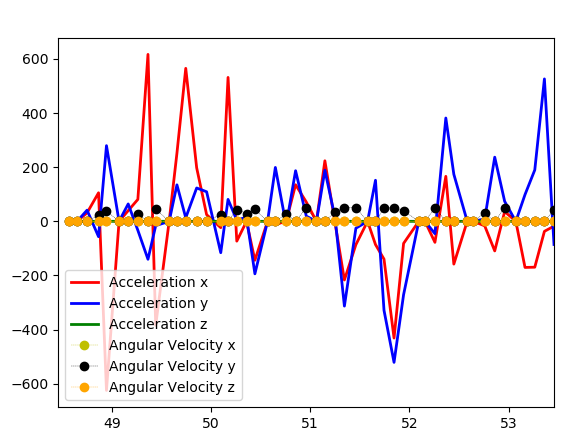
\includegraphics[width=.99\linewidth]{Bilder/IMU.png}
 		\caption{IMU data with acceleration and angular velocity}\label{fig_IMU}
 	\end{minipage}\hfill
 		\begin{minipage}[t]{0.48\textwidth}
		\centering
		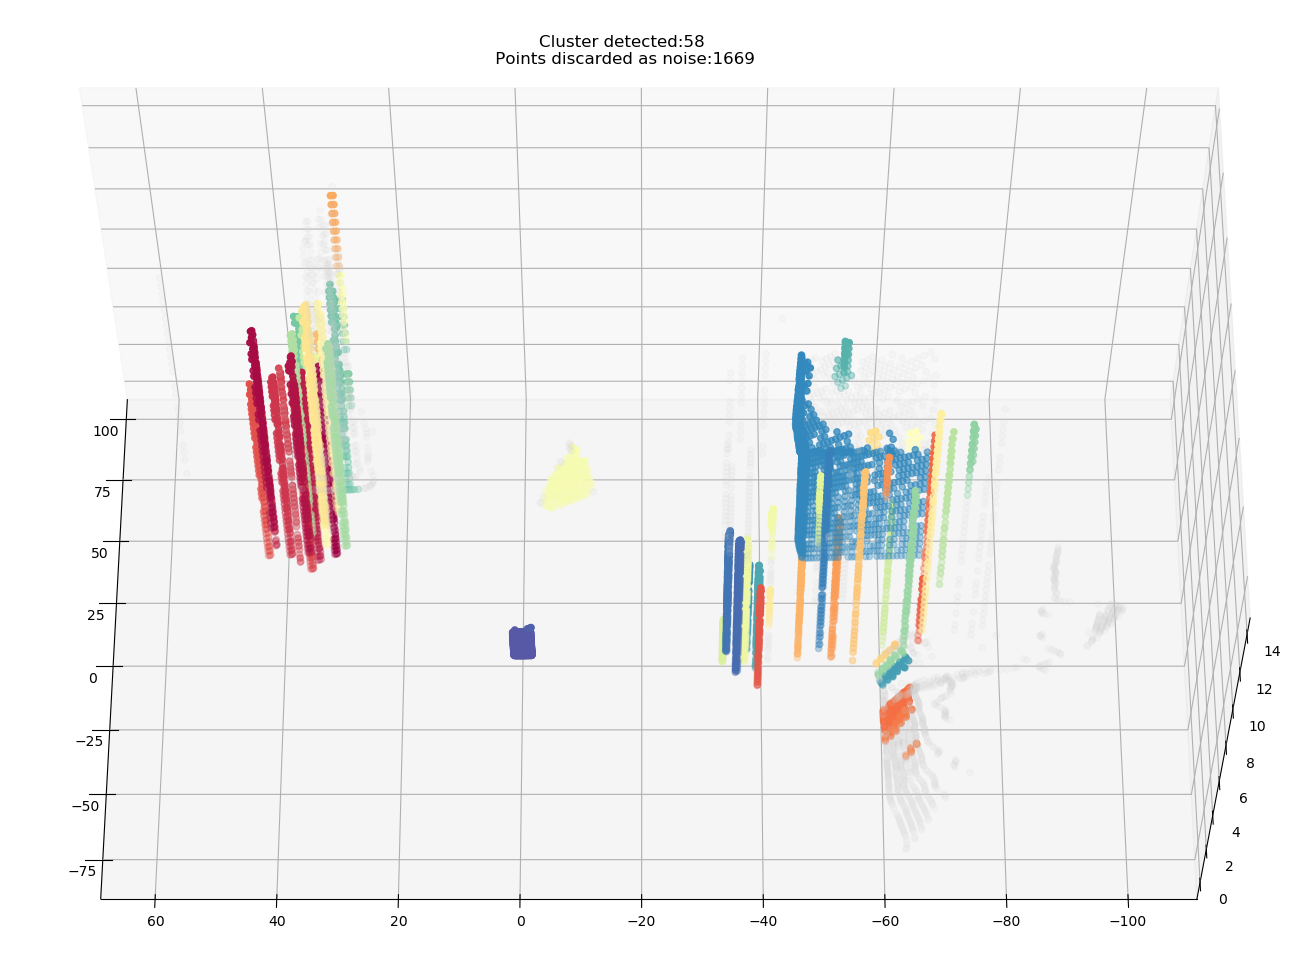
\includegraphics[width=.99\linewidth]{Bilder/LidarCluster.png}
		\caption{Lidar pointcloud with colored clusters}\label{fig_lidarMat}
	\end{minipage}
	
\end{figure}

As by clustering, the datasets size is not reduced apart from the neglected noise, the resolution of the clusters has to be reduced. That can be done by finding one or more shapes that enclose the cluster and thus includes all of its data. For reasons of simplicity only rectangluar shapes with a fixed orientation are used. In figure \ref{fig_lidarbox1} the black circles represent a two-dimensional cluster. The smallest rectangular shape with a fixed orientation parallel to $X$and $Y$ that includes all data points is the box that is set up by the lines $a,b,c$ and $d$. Being required to run in parallel to $Y$ the lines $a$ and $b$ are defined by the outmost position of points to the left and to the right respectively. Lines $c$ and $d$ run in parallel to $X$ and are defined by the highest and lowest point respectively in respect to the $Y$ axis. By dividing the resulting box into four even sized smaller boxes, the resolution of the cluster can be increased. As depicted in figure  \ref{fig_lidarbox2}, boxes that are not populated by points of the cluster can be discarded. Applied on the three-dimensionl lidar cluster, the boxes are intersected as long as they do not full fill the condition of being smaller than three meters in each dimension. For every resulting box it is checked whether there is a point inside the box. Boxes that contain points are then send to the \ac{ROS} network by taking their center and the extension in every dimension. \\

 \begin{figure}
 	\begin{minipage}[t]{0.48\textwidth}
	\begin{centering}
		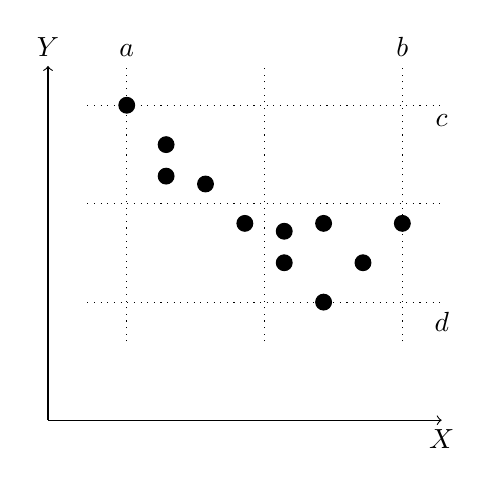
\begin{tikzpicture}      
		%\draw[help lines,xstep=.5,ystep=.5,dashed] (0,0) grid (6,6); %Hilfsdiagramm für Koordinaten
		%\foreach \x in {0,1 ,...,6} { \node [anchor=north] at (\x,0) {\x}; }
		%\foreach \y in {0,1,...,6} { \node [anchor=east] at (0,\y) {\y}; }
		
		\draw[->,] (0,0) -- 	(5,0) node  [at end,anchor= north]{$X$}; %x axis
		\draw[->,] (0,0) -- 	(0,4.5) node  [at end,anchor= south]{$Y$}; %z axis
		
		% sorted in rising x
		\draw[fill=black]       (1,4) circle (0.1) node (M)[below right]{}; % point M
		\draw[fill=black]       (1.5,3.5) circle (0.1) node (M)[below right]{}; % point M
		\draw[fill=black]       (1.5,3.1) circle (0.1) node (M)[below right]{}; % point M
		\draw[fill=black]       (2,3) circle (0.1) node (M)[below right]{}; % point M
		\draw[fill=black]       (2.5,2.5) circle (0.1) node (M)[below right]{}; % point M
		\draw[fill=black]       (3,2) circle (0.1) node (M)[below right]{}; % point M
		\draw[fill=black]       (3,2.4) circle (0.1) node (M)[below right]{}; % point M
		\draw[fill=black]       (3.5,1.5) circle (0.1) node (M)[below right]{}; % point M
		\draw[fill=black]       (3.5,2.5) circle (0.1) node (M)[below right]{}; % point M
		\draw[fill=black]       (4,2) circle (0.1) node (M)[below right]{}; % point M
		\draw[fill=black]       (4.5,2.5) circle (0.1) node (M)[below right]{}; % point M
	
		\draw[dotted] (1,1) -- 	(1,4.5) node  [at end,anchor= south]{$a$}; %left line
		\draw[dotted] (4.5,1) -- 	(4.5,4.5) node  [at end,anchor= south]{$b$}; %right line
		\draw[dotted] (0.5,1.5) -- 	(5,1.5) node  [at end,anchor= north]{$d$}; %bottom line
		\draw[dotted] (0.5,4) -- 	(5,4) node  [at end,anchor= north]{$c$}; %top line
		
		\draw[dotted] (0.5,2.75) -- 	(5,2.75) node  [at end,anchor= south]{}; %horizontal intersect
		\draw[dotted] (2.75,1) -- 	(2.75,4.5) node  [at end,anchor= north]{}; %vertical intersect
		
		
		\end{tikzpicture}
		\caption{Possible boxes to include data points of one cluster}
		\label{fig_lidarbox1}
	  \end{centering}
   	\end{minipage}\hfill
	\begin{minipage}[t]{0.48\textwidth}
	\begin{centering}
		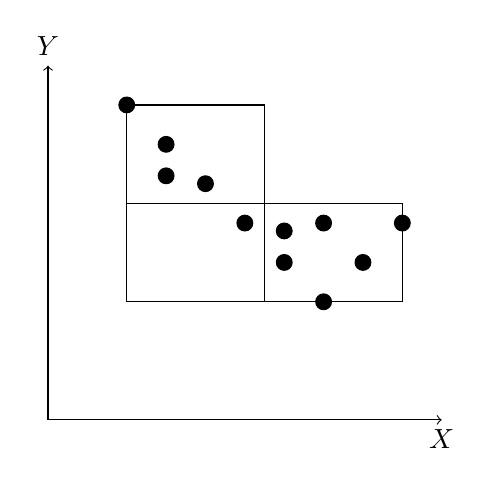
\begin{tikzpicture}      
		%\draw[help lines,xstep=.5,ystep=.5,dashed] (0,0) grid (6,6); %Hilfsdiagramm für Koordinaten
		%\foreach \x in {0,1 ,...,6} { \node [anchor=north] at (\x,0) {\x}; }
		%\foreach \y in {0,1,...,6} { \node [anchor=east] at (0,\y) {\y}; }
		
		\draw[->,] (0,0) -- 	(5,0) node  [at end,anchor= north]{$X$}; %x axis
		\draw[->,] (0,0) -- 	(0,4.5) node  [at end,anchor= south]{$Y$}; %z axis
		
		\draw[] (1,1.5) -- 	(1,4) node  [at end,anchor= south]{}; %left line
		\draw[] (4.5,1.5) -- 	(4.5,2.75) node  [at end,anchor= south]{}; %right line
		\draw[] (1,1.5) -- 	(4.5,1.5) node  [at end,anchor= north]{}; %bottom line
		\draw[] (1,4) -- 	(2.75,4) node  [at end,anchor= north]{}; %top line
		
		\draw[] (1,2.75) -- 	(4.5,2.75) node  [at end,anchor= south]{}; %horizontal intersect
		\draw[] (2.75,1.5) -- 	(2.75,4) node  [at end,anchor= north]{}; %vertical intersect
		
		% sorted in rising x
		\draw[fill=black]       (1,4) circle (0.1) node (M)[below right]{}; % point M
		\draw[fill=black]       (1.5,3.5) circle (0.1) node (M)[below right]{}; % point M
		\draw[fill=black]       (1.5,3.1) circle (0.1) node (M)[below right]{}; % point M
		\draw[fill=black]       (2,3) circle (0.1) node (M)[below right]{}; % point M
		\draw[fill=black]       (2.5,2.5) circle (0.1) node (M)[below right]{}; % point M
		\draw[fill=black]       (3,2) circle (0.1) node (M)[below right]{}; % point M
		\draw[fill=black]       (3,2.4) circle (0.1) node (M)[below right]{}; % point M
		\draw[fill=black]       (3.5,1.5) circle (0.1) node (M)[below right]{}; % point M
		\draw[fill=black]       (3.5,2.5) circle (0.1) node (M)[below right]{}; % point M
		\draw[fill=black]       (4,2) circle (0.1) node (M)[below right]{}; % point M
		\draw[fill=black]       (4.5,2.5) circle (0.1) node (M)[below right]{}; % point M
		\end{tikzpicture}
		\caption{Boxes resulting of discarded empty boxes of the cluster}
		\label{fig_lidarbox2}
	\end{centering}
\end{minipage}
\end{figure}
 
After receiving a \ac{RADAR} array with reflection values from Unity3d, its data is visualized in a \textit{matplotlib} plot in polar coordinate representation. Figure \ref{fig_RadarIntense} displays the resulting image. The byte typed array of reflection intensities is plotted for every cell from 0$\degree$ to 360$\degree$ with the according radius. To decrease the false alarm detection rate, a dynamic threshold is used in a next step to extract targets. The array that contains the detected signals is computed back to carthesian coordinates in order to obtain a general data format that was introduced by the \ac{LIDAR} data. It then is send to the \ac{ROS} network by taking the center of each detected signal.\\
 
In the scope of this work, only a two-dimensional collision mesh for the simulation of water is used and thus there are no wakes that can be falsely classified as a signal. Therefore the implementation of a \ac{OS-CFAR} algorithm is not required and the \ac{SOCA-CFAR} is used. However, in more sophisticated simulations or real world applications where situations can be expected in which many objects have to be detected that are in close proximity to each other, the \ac{OS-CFAR} is the algorithm of choice. Additionally, with the ability to model the strength of wakes with the Rayleigh \ac{PDF}, the \ac{OS-CFAR} provides further chances to reduce the false alarm rate.\\

Especially in artificially confined spaces with defined borders an algorithm that detect lines in the scenes images can provide useful information to specify the environment. In order to detect lines, the edges of the image have to be extracted. For that 
the python library OpenCV with a focus on real time applications for computer vision provides the so called Canny Edge Detection function. To extract edges, first a Gaussian filter is applied on the greyscale image to reduce noise. In a next step the edge gradients in vertical and horizontal directions are computed. The function allows for choosing the number of pixels that are included in the calculation for each gradient. If the gradient value is above a threshold one, the position is considered as an edge. If its below a threshold two, the value is discarded. For the values in between the two thresholds, the decision whether an edge is present or not is dependent on the existence of values above threshold two in the neighbourhood. The resulting edge image can be passed to the Hough-algorithm which then extracts the lines. Figure \ref{fig_Houghlines} visualizes the result of a line extraction applied to the image from the image sensor. Three blue lines indicate the detection of lines from an image, that has been passed to a edge detection beforehand. As the serialization of bytes is not implemented in the \textit{rosbridgelib} that connects Unity3d with ROS2, the image is saved in the underlying Linux filesystem. Only a message that indicates the availability of a new image and the place where it is saved is published in the ROS2 network. After the according \ac{ROS} node receives the message, the image is read from the specified storage place and can be processed.


\begin{figure}[!htb]
	\begin{minipage}[t]{0.48\textwidth}
		\centering
		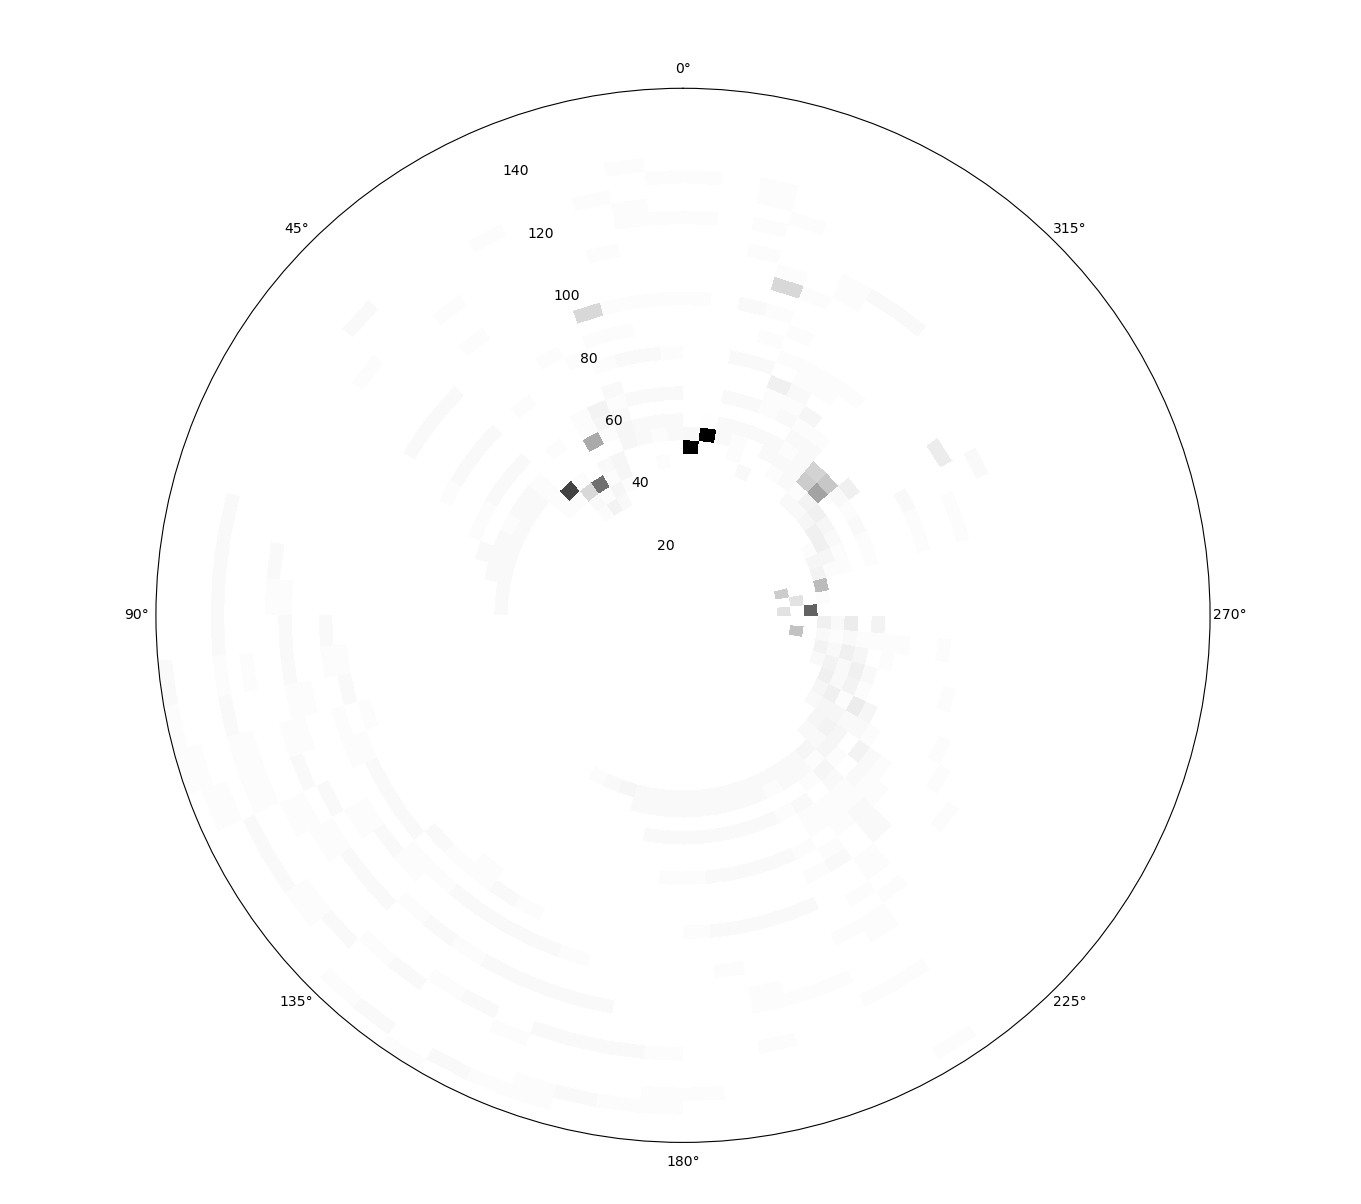
\includegraphics[width=.9\linewidth]{Bilder/RadarIntensity.png}
		\caption{Radar data with reflection intensity}
		\label{fig_RadarIntense}
	\end{minipage}\hfill
	\begin{minipage}[t]{0.48\textwidth}
		\centering
		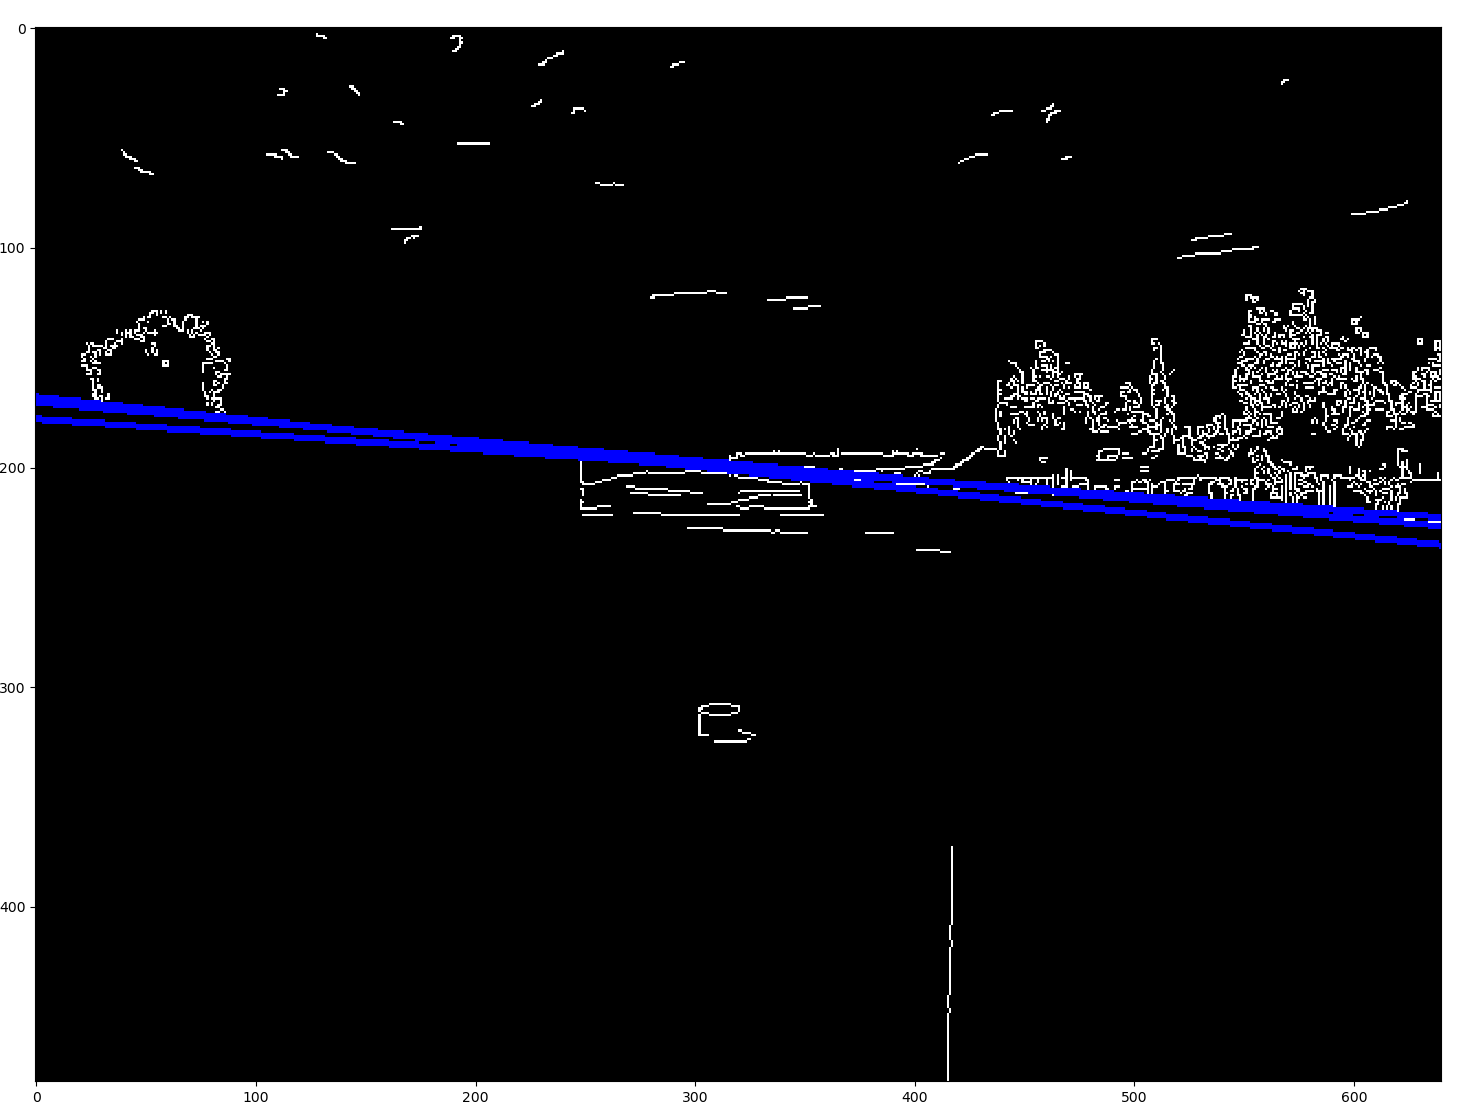
\includegraphics[width=.9\linewidth]{Bilder/houghlines.png}
		\caption{Edge image with visualized hough line detection in blue }
		\label{fig_Houghlines}
	\end{minipage}
\end{figure}

As a last step, the processed information of the \ac{LIDAR} and \ac{RADAR} are displayed together. Figure \ref{fig_RvizBird} displays the \ac{RADAR} data in red circles together with the \ac{LIDAR} data in yellow rectangles from a perspective above the scene. Figure \ref{fig_RvizThird} displays the same state of the scene from a third person perspective. The aforementioned bounding boxes of the \ac{LIDAR} data become visible in yellow with the size of a single box not exceeding a certain limit. The sensor center is indicated by  small coordinate system arrows in the center of the figure. Around the arrows the shape of the small vessel is displayed. The two dimensional \ac{RADAR} data is visualized with red cylinders. 
 \begin{figure}[!htb]
	\begin{minipage}[t]{0.48\textwidth}
		\centering
		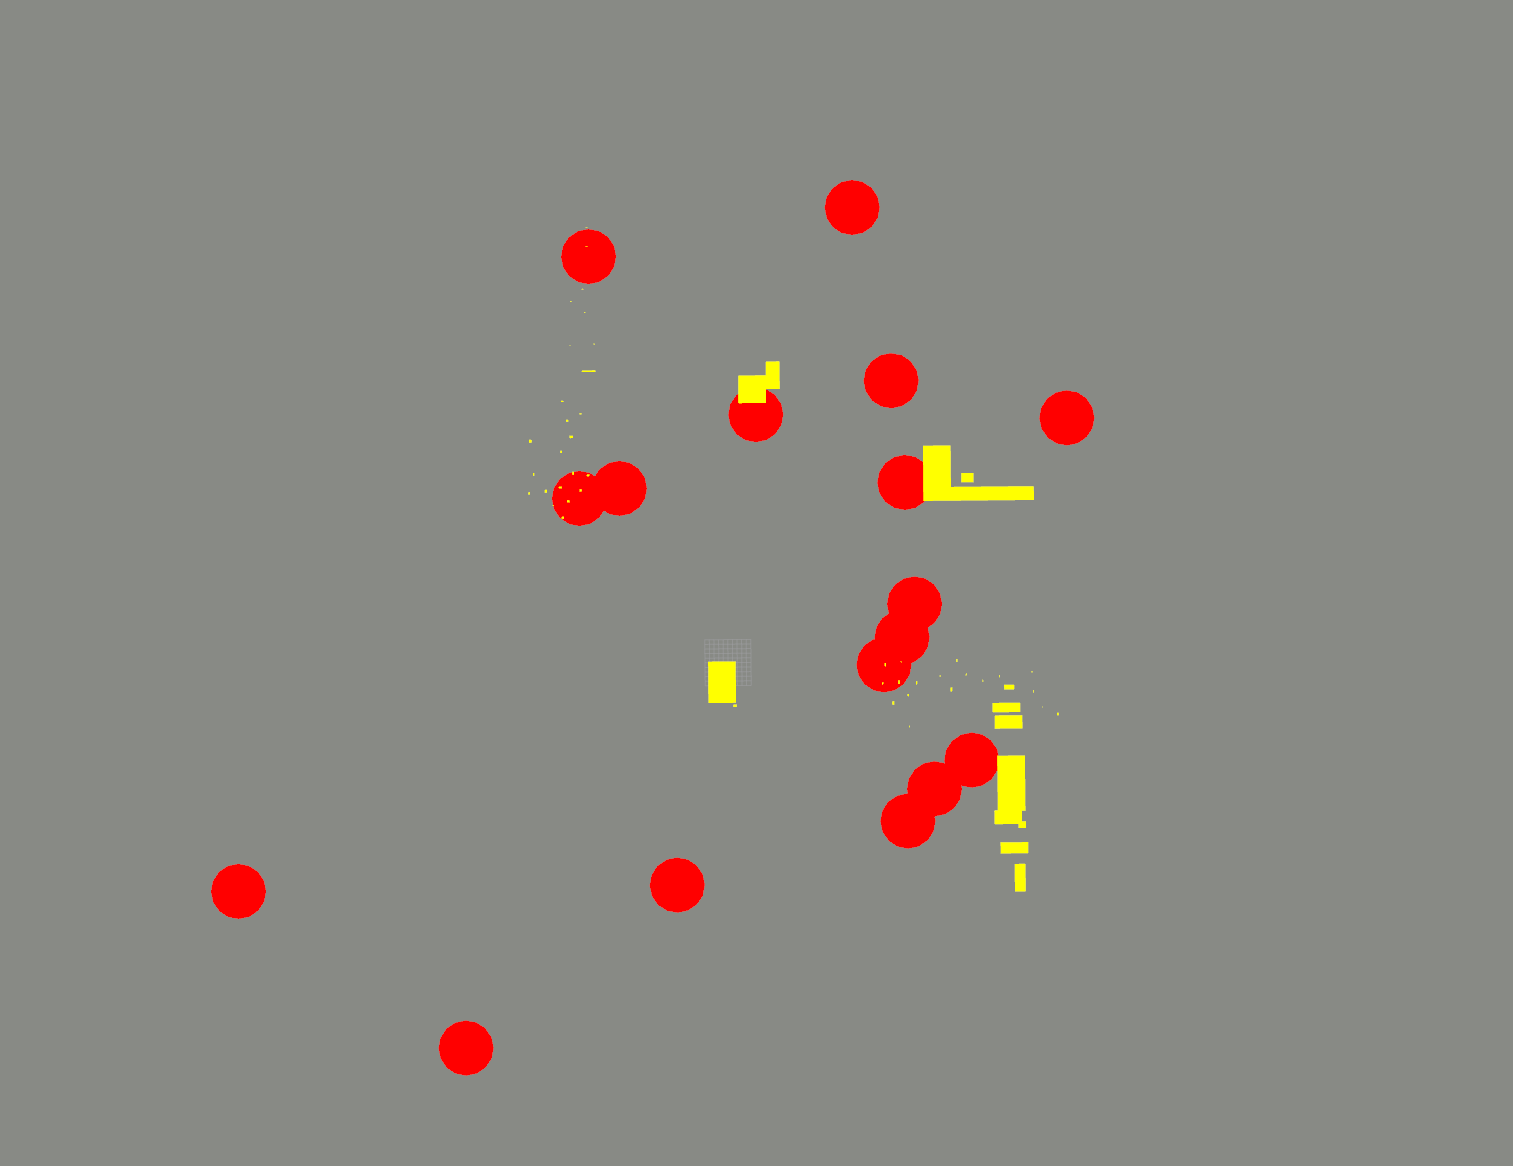
\includegraphics[width=.9\linewidth]{Bilder/Objectmap.png}
		\caption{Lidar (yellow) and radar (red) objects from above}\label{fig_RvizBird}
	\end{minipage}\hfill
	\begin{minipage}[t]{0.48\textwidth}
		\centering
		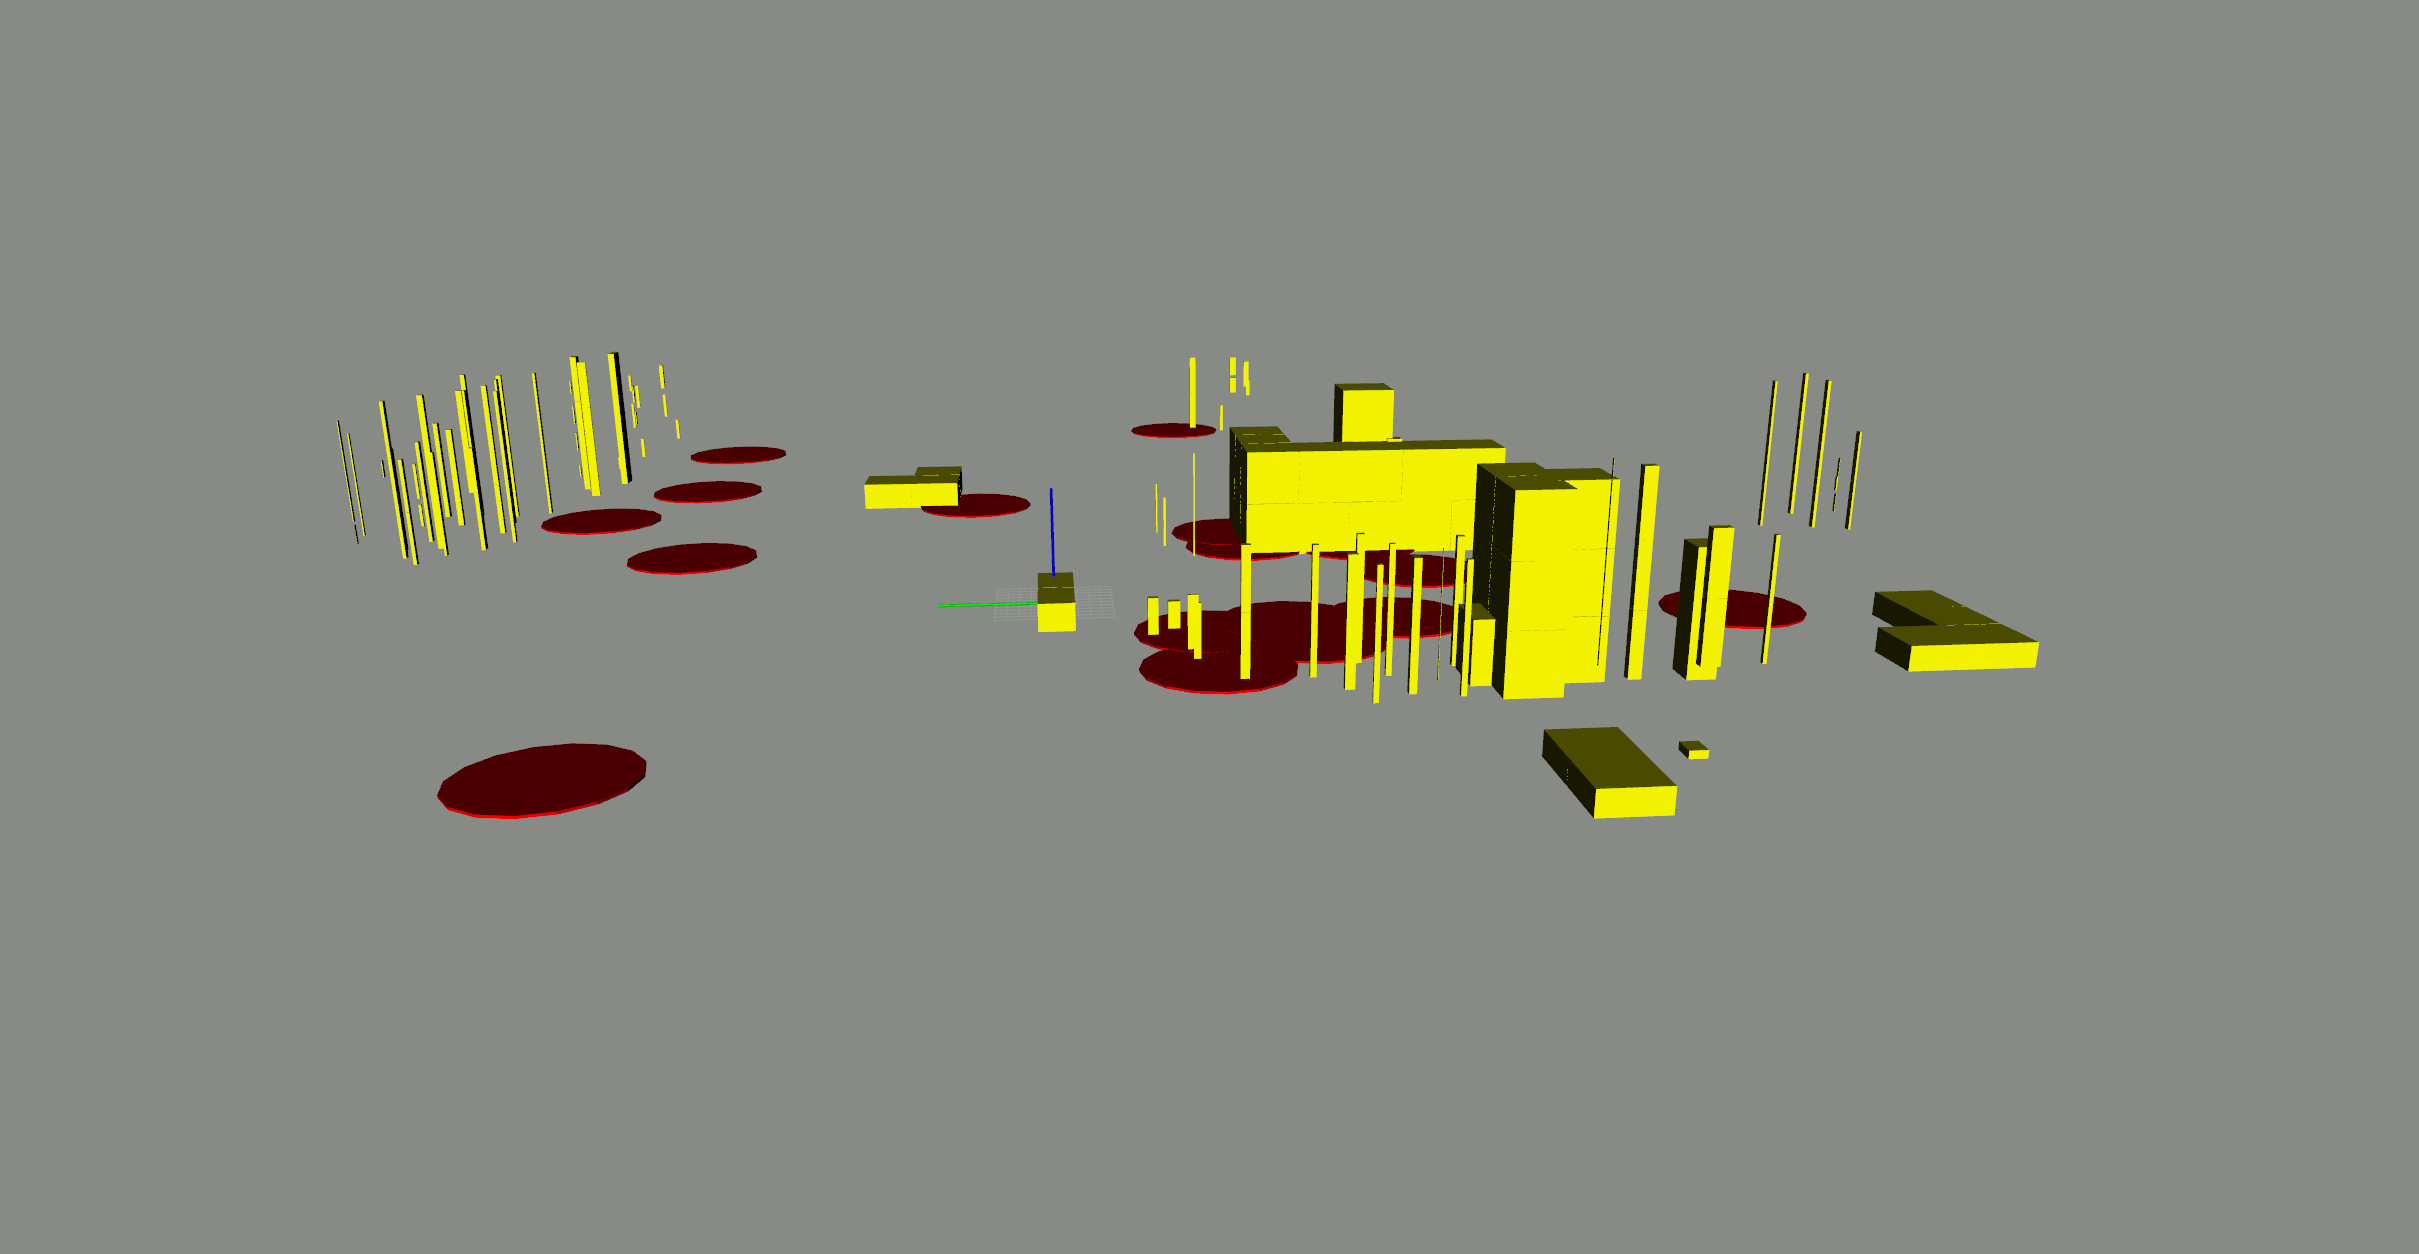
\includegraphics[width=.9\linewidth]{Bilder/RvizThirdPerson.png}
		\caption{Lidar and radar objects in third person perspective}\label{fig_RvizThird}
	\end{minipage}
\end{figure}
%\begin{figure}
%	\centering
%	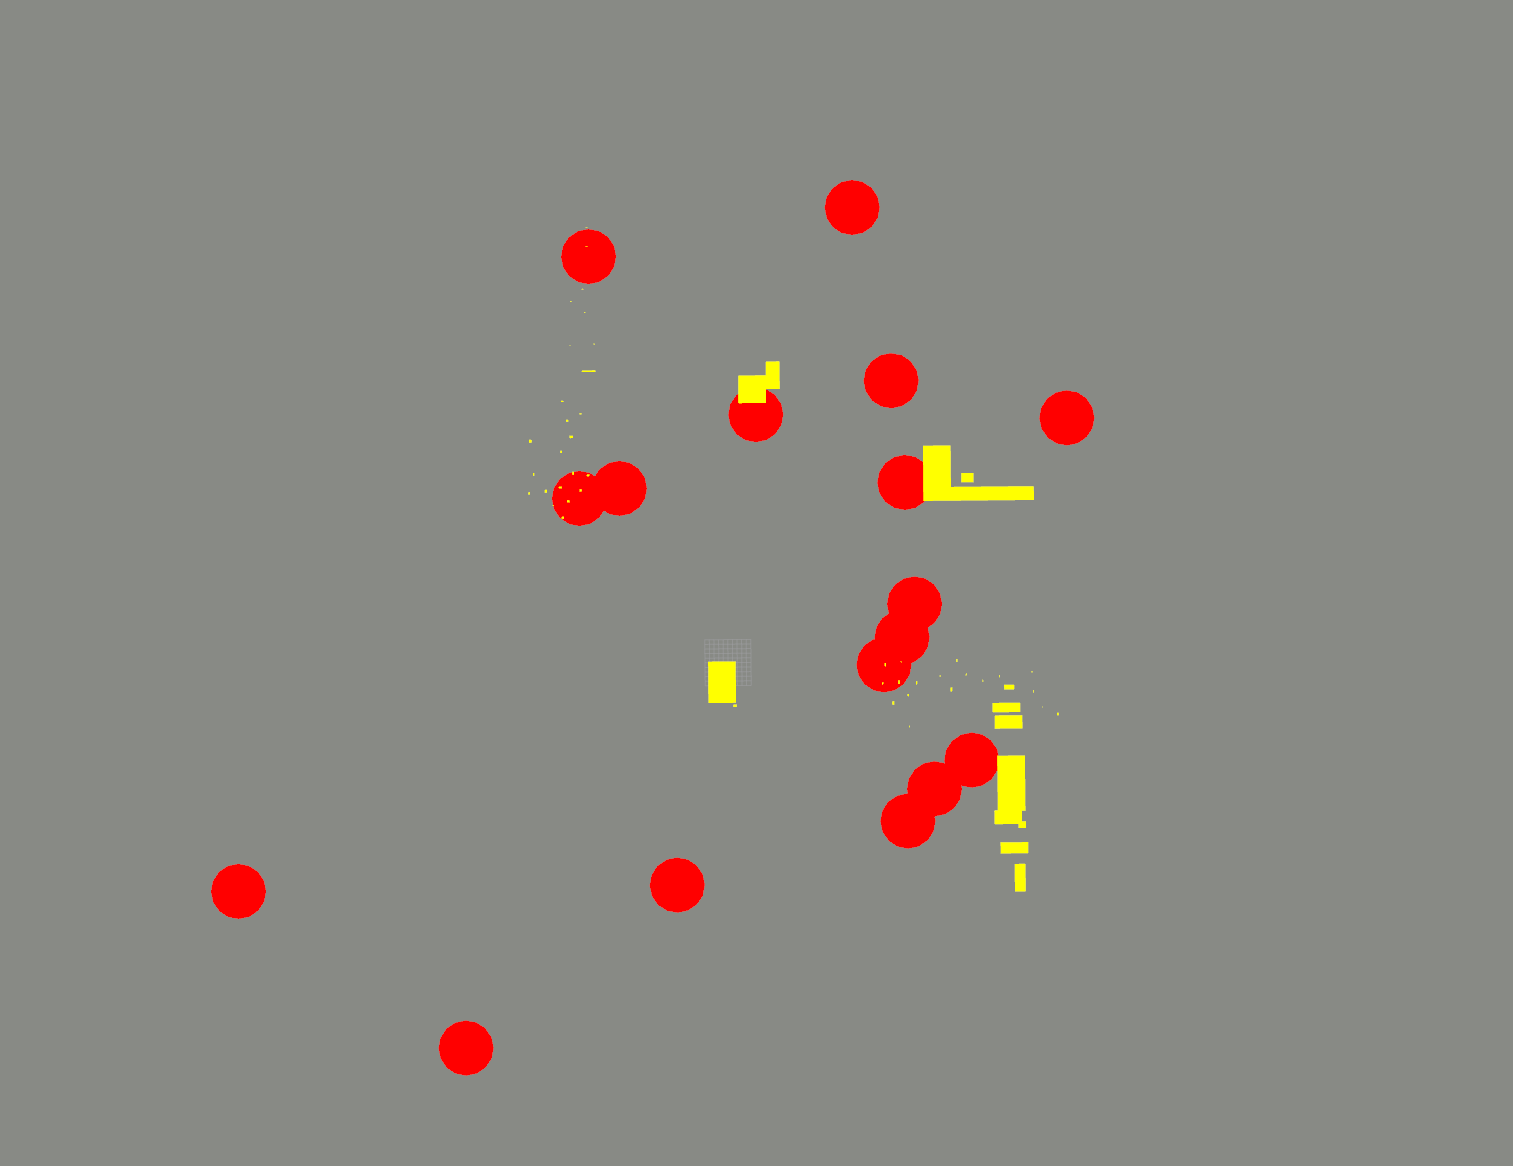
\includegraphics[width=10cm]{Bilder/Objectmap.png}
%	\caption{Lidar (yellow) and radar (red) objects from above}\label{fig_RvizBird}
%\end{figure}
%\begin{figure}
%\centering
%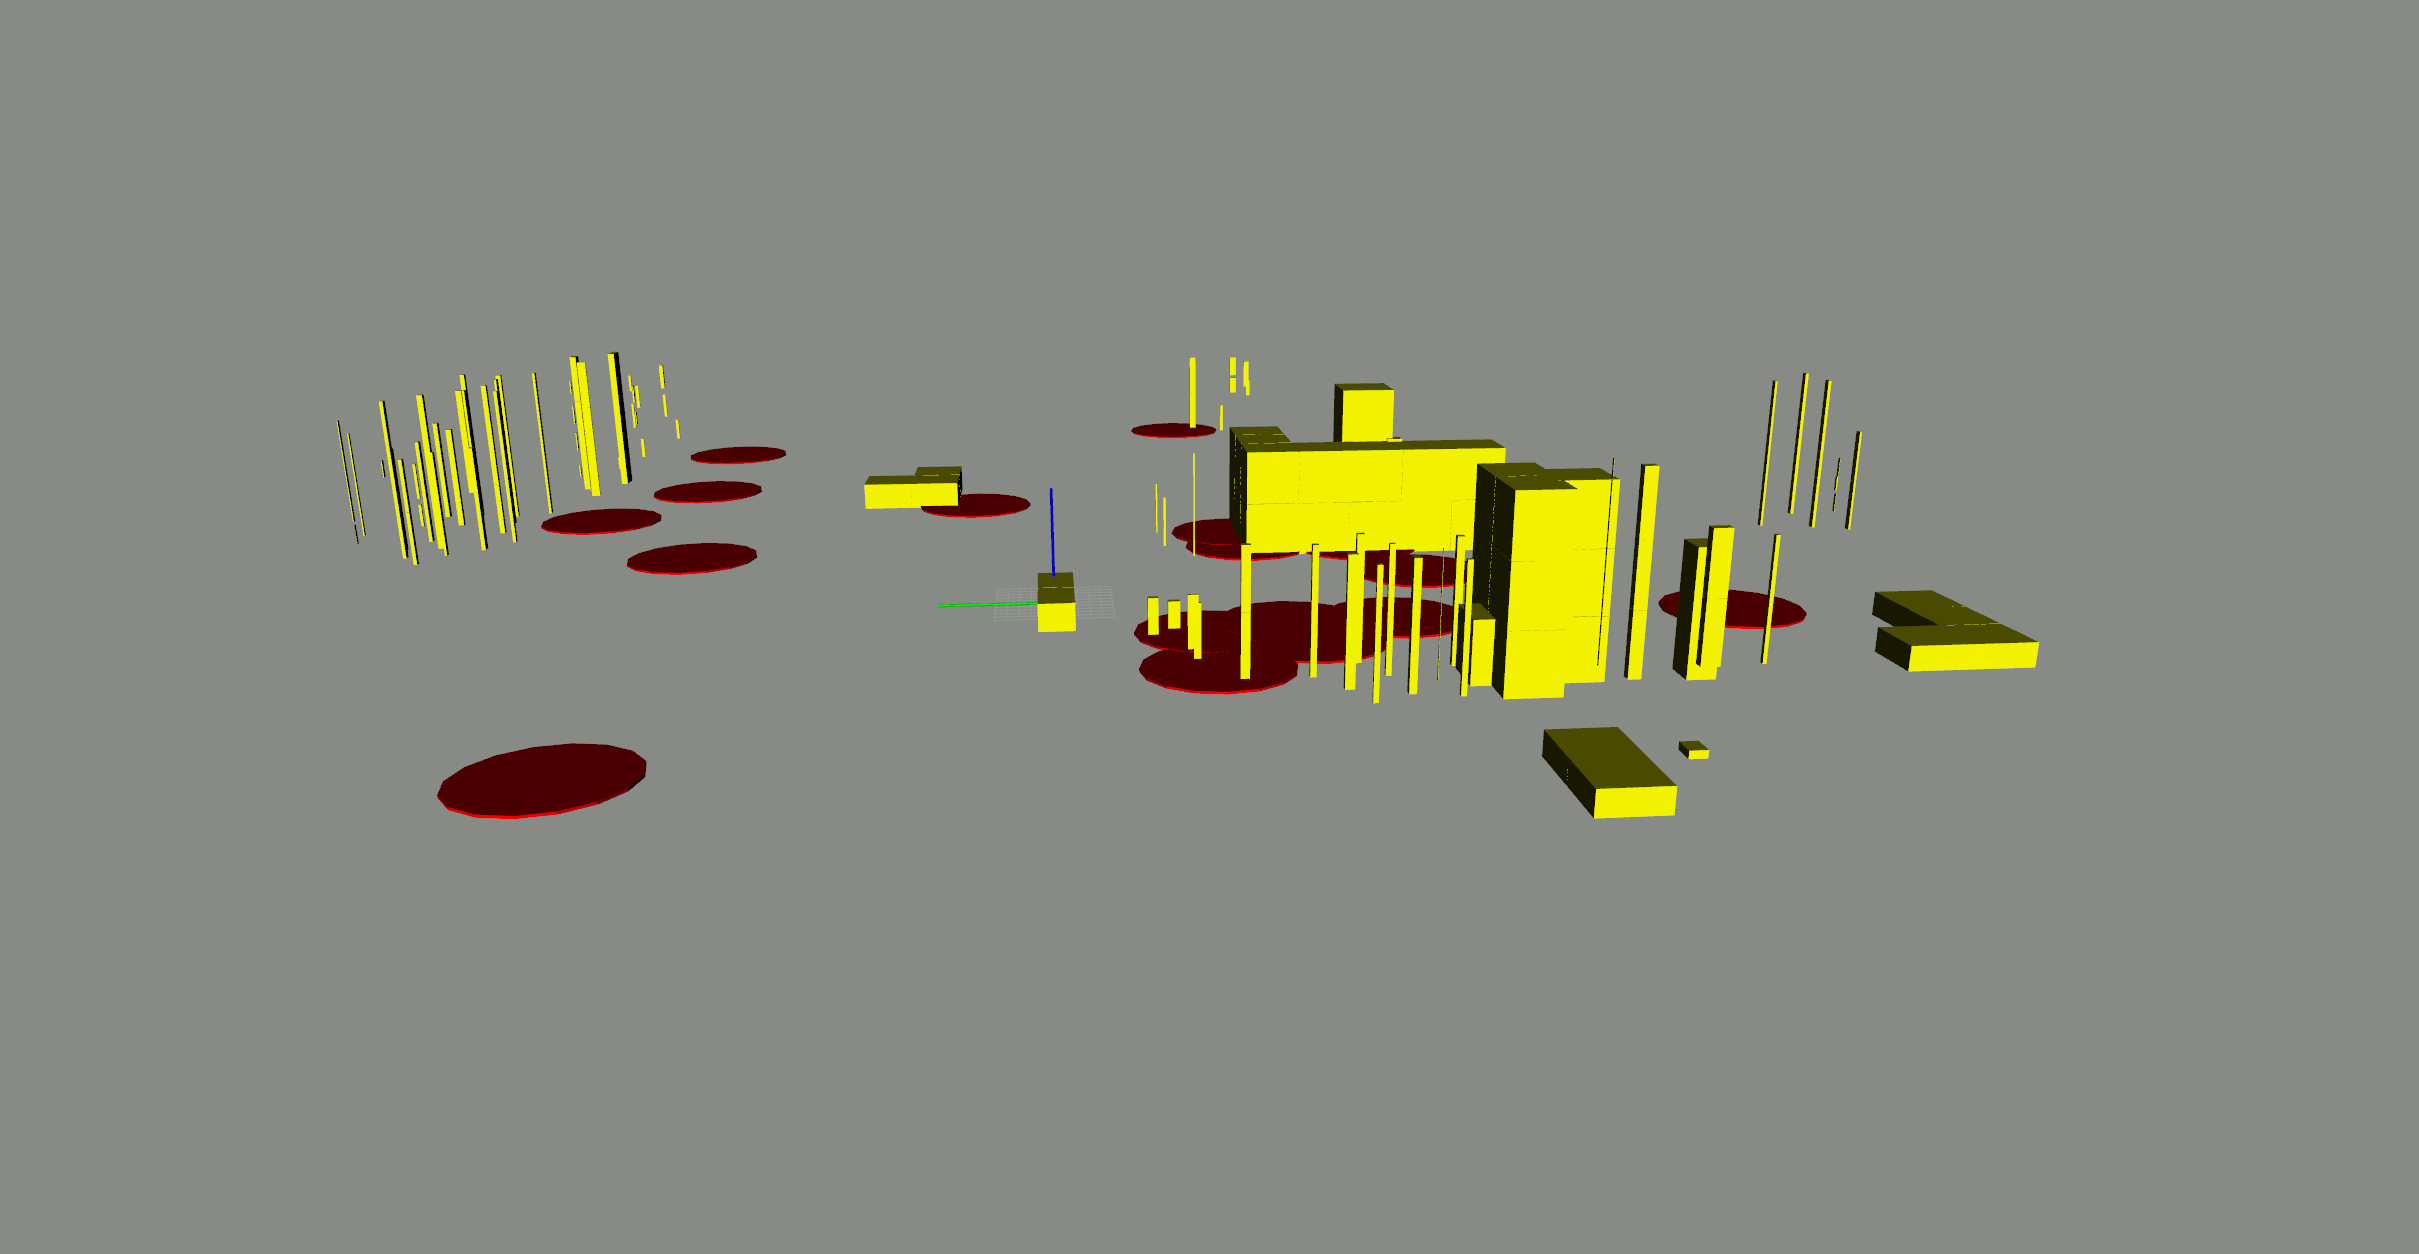
\includegraphics[width=10cm]{Bilder/RvizThirdPerson.png}
%\caption{Lidar and radar objects in third person perspective}\label{fig_RvizThird}
%\end{figure}



  \chapter{Results and Discussion} \label{Result}
 With the suitable algorithms implemented, in this section the parameters of the algorithms are further discussed. As the data of the virtual sensors are dependent on its preferences in the Unity3d scene, they are documented in subsection \ref{Parameters}. Subsequently the performance of the system is evaluated by taking the latency of every processing step. The tests are strongly focused on the median latency and reliability in terms of timing inaccuracies and scattering of the data generation, transmission and processing. The tests that are conducted in the following can be divided into the test of the modules which goes along with the integration of the modules in subsection \ref{latency}, the test to proof the successful integration of parts in subsection \ref{intpart} and the validation of the software as a whole in subsection \ref{validate}.
 
 \section{Sensor Parameters} \label{Parameters}
 The virtual sensors as implemented in the Unity3d scene have to generate data about its digital environment by reproducing the physical properties of real sensors. Inherent to this approach is the limitations that are set by the processing power of the unit that calculates the virtual sensors data. Therefore, in addition to the values that can be derived from real sensors, the performance of the system has to be observed when for example increasing the resolution of a sensor to resemble an analogous sensor signal by means of discrete digital values. The settings of the sensors and data processing algorithms values are determined experimentally and merely provide an example for the possibilities of the overall system architecture. Therefore in the following the validation of the values is conducted on a qualitatively basis without comparing the performance effects of different sensor settings. \\
 
 The resolution of the virtual \ac{RADAR} is an example for the necessity to deviate from the real sensor as proposed before. To realize an object detection in a range of several kilometres with a detection rate that equals that of an analogous \ac{RADAR}, the digital \ac{RADAR}'s angular resolution exceeds the processing power of a common computer. Thus its detection range is limited to about 100m for objects below four meters in the current implementation. Table \ref{tab_radarsens} provides an overview of the settings of the \ac{RADAR}. One beam of the \ac{RADAR} is five degrees wide in azimuth and 15$\degree$ wide in altitude. The resolution of one beam is 30x2 raycasts. For the detection of objects close to the \ac{RADAR}'s origin the resolution proved to be sufficiently detailed. However, after exceeding a certain range, small objects are able to pass the \ac{RADAR}'s rays undetected due to the increasing space between subsequent rays. To increase the detection rate of objects, providing them with a very high reflection value of about 100 provided good results when applying the \ac{SOCA-CFAR} filter.\\ 
 
 The settings of the filter that proved to be most effective are documented in table \ref{tab_filter}. A total of 100 cells are taken into consideration to compute the decision whether the \ac{CUT} is classified as an target object or not. Ten cells that are five to the right and five to the left of the \ac{CUT} are ignored and thus decrease the chance that signals of objects are taken into consideration when computing the noise average. The false detection rate is set to 0.1. In contrast to a fixed threshold, the \ac{SOCA-CFAR} provides usable results even when changing the settings of the virtual \ac{RADAR} which for example results in an increased overall reflection value. That can be considered as an effect of the dynamic threshold    calculation.                                                                                                                                                                                                                                                                                  
  
  \begin{figure}[!htb]
 	\begin{minipage}[t]{0.48\textwidth}	
 		\begin{table}[H]	
 			\centering
 			\caption{\ac{RADAR} sensor values}
 			\begin{tabular}{l l } 
 				\midrule\midrule
 				Unity3d  & Value\\ 
 				\midrule
 				Cell Azimuth Extension  &5.0\\
 				Cell Extension & 4  \\
 				Cell Altitude Extension & 15\\
 				Burst Vertical Resolution & 30\\
 				Burst Horizontal Resolution & 2
 			\end{tabular}
 			\label{tab_radarsens}
 		\end{table}
 	\end{minipage}\hfill
 	\begin{minipage}[t]{0.48\textwidth}
 		\begin{table}[H]
 			\centering
 			\caption{Filtering values}
 			\begin{tabular}{l l } 
 				\midrule\midrule 
 				SOCA-CFAR  & Value\\ 
 				\midrule
 				Training Cells&100 \\	
 				Guard Cells&10 \\
 				False Detection Rate& 0.1
 			\end{tabular}
 			\label{tab_filter}
 		\end{table}
 	\end{minipage}
 \end{figure}
 The physical principle of operation of the \ac{LIDAR} allows virtual data generation without further transformation and approximation. Thus, the data generation in the simulation can forgo without substantial compromises. As listed in table \ref{tab_lidarsens} the \ac{LIDAR} is set to about 345000 points with a frequency of two Hertz. The horizontal and vertical resolution are 0.25$\degree$ per ray with an field of view of 360$\degree$ and 60$\degree$ respectively. The procession of the points with the \ac{DBSCAN} algorithm yields the most promising results with the settings in table \ref{tab_cluster}. The values have been determined experimentally with adjustments taken in comparison with the objects spatial limitations as visible in the Unity3d scene. An $Eps$ value of one equals to points being considered as neighbours with an distance of below one meter to each other. $MinPts$ set to ten indicates that a minimum of ten points is required in a cluster to be considered as such. The resolution of the bounding box is a further value that can be set. With applications prioritising accuracy, the resolution can be set higher and thus allow for boxes that frame the data more precisely. However, in situations that require a highly responsive system, compromising the accuracy by decreasing the resolution to higher bounding box values can lead to a higher performance in terms of processing time. The value of three that equals to three meters provides a sufficient accuracy without using to much processing time.
 \begin{figure}[!htb]
 	\begin{minipage}[t]{0.48\textwidth}	
 		 \begin{table}[H]	
 			\centering
 			\caption{\ac{LIDAR} sensor values}
 				\begin{tabular}{l l } 
 				\midrule\midrule
 				Unity3d  & Value\\ 
 				\midrule
 				Horizontal Resolution	& 0.25\\
 				Vertical Resolution& 0.25 \\
 				Vertical Field of View	& 60\degree
 				\end{tabular}
 			\label{tab_lidarsens}
 		\end{table}
 	\end{minipage}\hfill
 	\begin{minipage}[t]{0.48\textwidth}
 		 \begin{table}[H]
 			\centering
 			\caption{Clustering values}
 				\begin{tabular}{l l } 
	 			\midrule\midrule 
 				DBSCAN  & Value\\ 
 				\midrule
 				Eps&1 \\	
 			    MinPts&10 \\\\
 			    
 				\midrule\midrule
 				Bounding Box & Value\\
 				\midrule
 				Resolution & 3
 				\end{tabular}
 			\label{tab_cluster}
 		\end{table}
 	\end{minipage}
 \end{figure}
 By choosing the resolution and compression of the rendered image from the Unity3d scene, the data size of the visual environment information can be reduced or increased. As shown in table \ref{tab_imagesens}, 640 pixel in width and 480 pixel in height are chosen as values for the image resolution together with a jpeg compression. These values provide enough details for the subsequent line extraction and at the same time allow for an acceptable procession time. For the edge detection and line extraction, table \ref{tab_extraction} provides information of the used variables. The algorithm for the edge detection as proposed by Canny uses 170 for a first threshold and 260 as a second threshold. With an value above one for $Rho$ as the distance in pixels between sampled pixels and a $Theta$ of one as the angular distance in which lines through edge points are computed, the Hough algorithm provides a sufficient computation time. To decrease the false alarm rate, the $Threshold$ is set to 190. Increasing this value results in a higher amount of lines with the same value in the Hough feature space for an edge to be considered a line in the Hough image space.
 \begin{figure}[!htb]
	\begin{minipage}[t]{0.48\textwidth}	
		\begin{table}[H]	
			\centering
			\caption{Image sensor values}
			\begin{tabular}{l l } 
				\midrule\midrule
				Unity3d  & Value\\ 
				\midrule
				Width & 640 \\
				Height & 480 \\
				Compression & Jpeg\\
				
			\end{tabular}
			\label{tab_imagesens}
		\end{table}
	\end{minipage}\hfill
	\begin{minipage}[t]{0.48\textwidth}
		\begin{table}[H]
			\centering
			\caption{Line extraction values}
			\begin{tabular}{l l } 
				\midrule\midrule 
				Canny  & Value\\ 
				\midrule
				Threshold 1 &170 \\	
				Threshold 2 & 260 \\
				\midrule\midrule 
				Hough  & Value\\ 
				\midrule
				Rho & 1.1 \\	
				Theta & 1\degree\\
				Threshold & 190
			\end{tabular}
			\label{tab_extraction}
		\end{table}
	\end{minipage}
\end{figure}



	\section{Module and Module Integration Test}\label{latency}
	The specifications of the hardware that is used to test the system is given in table \ref{tab_hardware}. With 30 GiB of random access memory, 16 cores at 3.60 GHz and a RTX series graphics card, the system can be considered as being up to date. As an operating system Ubuntu LTS is used. This Linux derivative has the advantage that it is supported by \ac{ROS2} as well as Unity3d.	
	
	\begin{table}[H]
		\centering	
		\caption{Hardware used for testing}
		\begin{tabular}{l l } 
			\toprule
			Category  & Type\\ 
			\midrule
			Processor & 			Intel Core i9-9900KF CPU @ 3.60GHz x 16 \\ 
			Random Access Memory & 	30GiB\\
			Graphics Card & 		Nvidia TU104 GeForce RTX 2070 SUPER\\
			Operating System & 		20.04.2 LTS Ubuntu\\
			\bottomrule	
		\end{tabular}
		\label{tab_hardware}
	\end{table}

	To test the modules that are represented by methods in Unity3d and ROS2, the time each method takes to be executed is saved multiple times. As the system modules are dependent on each other, the test is executed with a function-able system without executing single methods in an isolated environment. Therefore, module and integration test are conducted simultaneously. Table \ref{tab_abb} in appendix \ref{Attachtable} depicts the single methods and average times of execution of these methods. As a benchmark for the execution time in the Unity3d system, the default physics engine update time of 20ms is used. Values below 20ms allow an event calculation as intended by the engine and enable Unity3d to render a consistence visual simulation representation. The benchmark of the \ac{ROS2} process time is the frequency of the sensors data generation e.g. the \ac{LIDAR} sensor is set to 2 Hertz.\\
	
    The processor and \ac{GPU} utilization in the system during the tests is shown in table \ref{tab_cpuload}. For the CPU, the load in three system states is taken with the tool \textit{htop}. With a total of 16 cores, a value of 16 results in the CPU being full loaded. Values above 16 result in queued processes. The system in idle mode uses 60\% of one core and the system with an active Unity3d simulation and running ROS2 nodes uses six cores and 56 \% of the seventh core. Regarding the GPU load that is measured with \textit{nvidia-smi}, only 49\% is used with Unity3d and ROS2 running. It can be stated, that the CPU and GPU processing power constitute no limitation for conducting tests on the system.
		
		\begin{table}[H]
		\centering	
		\caption{CPU and GPU load}
		\begin{tabular}{l l } 
		\midrule\midrule 
		System processes & CPU Load (max 16) $\varnothing1min$\\ 
		\midrule
		Idle			 & 0.6 \\	
		Unity3d 		 & 3.91 \\
		Unity3d and ROS2 & 6.56 \\
		\midrule\midrule
		System processes & GPU Load (max 100\%)\\
		\midrule
		Unity3d and ROS2 & 49\% \\
	\end{tabular}
		\label{tab_cpuload}
	\end{table}

	To test the implementation of the modules in the system, the average execution time of the methods for the \ac{IMU}, Image, \ac{RADAR} and \ac{LIDAR} in Unity3d and \ac{ROS2} is taken. Figure \ref{fig_time} depicts these values. In the first category with execution times from (a) to (d), the methods for the \ac{IMU} data (a) equals to zero as the average is below the vertical axis that is logarithmic scaled in milliseconds. (a), (b) and (c) are below the 20ms with which Unity3d updates its physics per default. The calculation of the \ac{LIDAR} data (d) exceeds 20ms with a value of 69ms. This makes a more detailed analysis  necessary to narrow down on the methods that are responsible for the high computation time.\\
	
	The second category in figure \ref{fig_time} is represented by the \ac{ROS2} subsystem. The according values for (e) to (h) represent the time that is required to process and visualize the data of the sensors. With a value of above 72ms, the \ac{IMU} (e) with an update rate of 50 Hertz exceeds its benchmark value of 20ms values by 52ms. The same counts for the calculation of the \ac{LIDAR} data (h). With an update rate of 500ms, the processing time surpasses the defined benchmark by 517ms. Both the methods of (e) and (h) are looked upon in greater detail in the following. (f) and (g) can be considered as performing well in comparison to its update rate of 500ms. 
	\begin{figure}
		\begin{centering}
			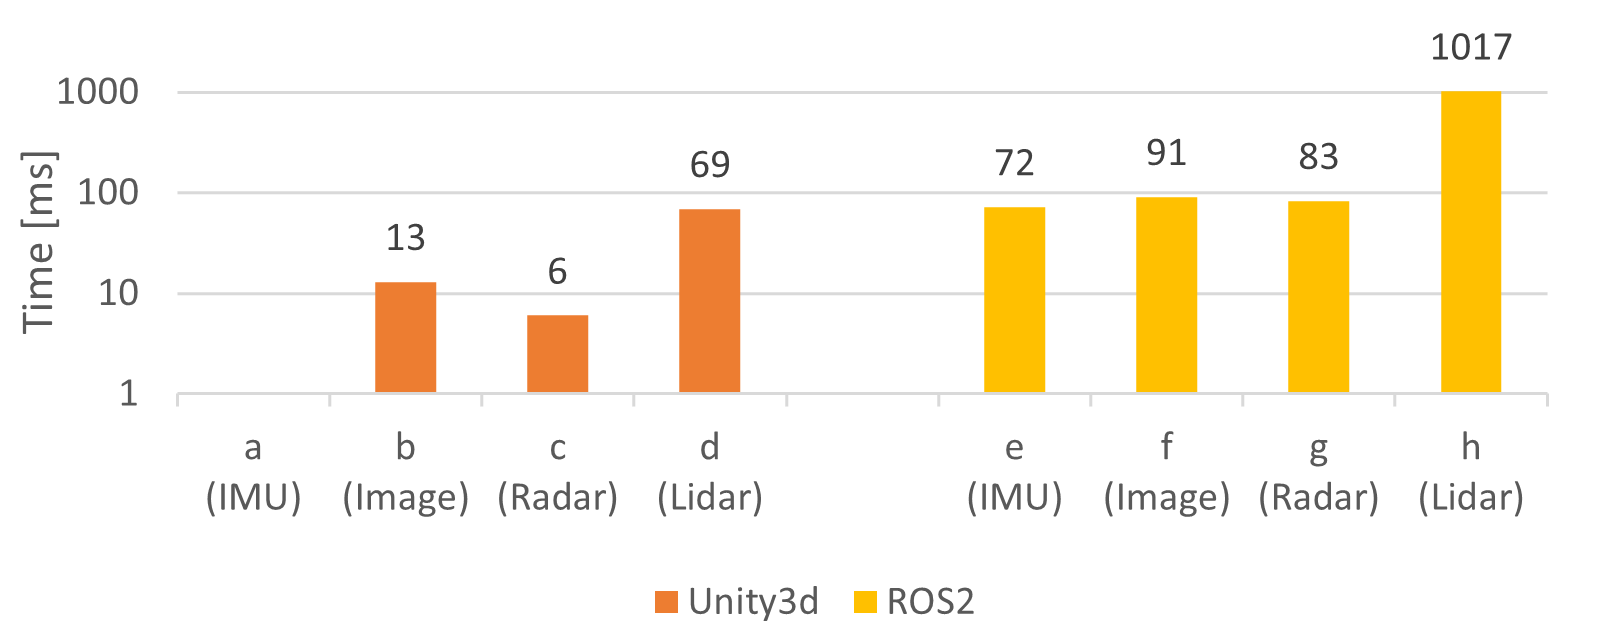
\includegraphics[width=0.75\textwidth]{Bilder/Time.PNG}
			\caption{Methods average execution time (total of 165000 execution)}
			\label{fig_time}%Label für das Referenzieren 
		\end{centering}
	\end{figure}
	
	Figure \ref{fig_Unity3d1} provides more detailed information about the execution time of methods in Unity3d with a box and whisker plot. The figure is divided into two plots with the plot to the left describing the methods execution time in milliseconds up to 18 milliseconds and the plot to the right methods with a longer execution time up to 180 milliseconds. A total of fourteen methods of the categories Radar, Image, \ac{IMU} and Lidar are investigated over a total of 126000 executions with an update frequency of two Hertz with the \ac{IMU} being an exception with 50 Hertz. In the plot to the left, the raycast of the \ac{RADAR} (1b) takes the longest time by comparison of medians. However, with 4 milliseconds this value can be considered as sufficient low compared to the time of 20ms with which the the physics engine of Unity3d calculates new data per default. In terms of reliability, there are outliers which are higher than the 4ms of (1b). This is of importantance in particular as they compromise the reliability of data generation in a fixed time. Especially publishing the \ac{IMU} data (1i) stands out in terms of difference from the median to the outliers. The longest execution time of (1i) is around 17ms. However, when using the benchmark of the repetition rate of the physics update, this value can be considered as sufficiently fast to avoid missing physics events.\\
	
	The plot to the left depicts the three most time consuming methods on Unity3d with the data generation of the \ac{LIDAR} (2a), publishing the data of the \ac{LIDAR} (2b) and generation i.e. rendering of the image. By exceeding the physics update repetition rate, methods (2a) and (2c) show a very limited range of the times of the outliers. In contrast executing (2c) can take up to 170ms with a median of 13ms. It can be assumed that for the three outliers that are considerably higher than the median an exception occurs e.g. other processes are scheduled to be executed on the same processor core as (2c). To summarize, for a higher performance in Unity3d, (2b) has to be optimized towards a higher overall performance and modifications in the system should lead to avoidance of the peak values of (2c).\\
	
	%However, as the update frequency of (2a),(2b) and (2c) is two Hertz, the implementation as tested is sufficient for the application with the backdraw of missing some physic events and visual representations. This effect should be minded for appliances that require a simulation  \\ 
	
	\begin{figure}
		\begin{center}
			\resizebox{.9\textwidth}{!}{%
				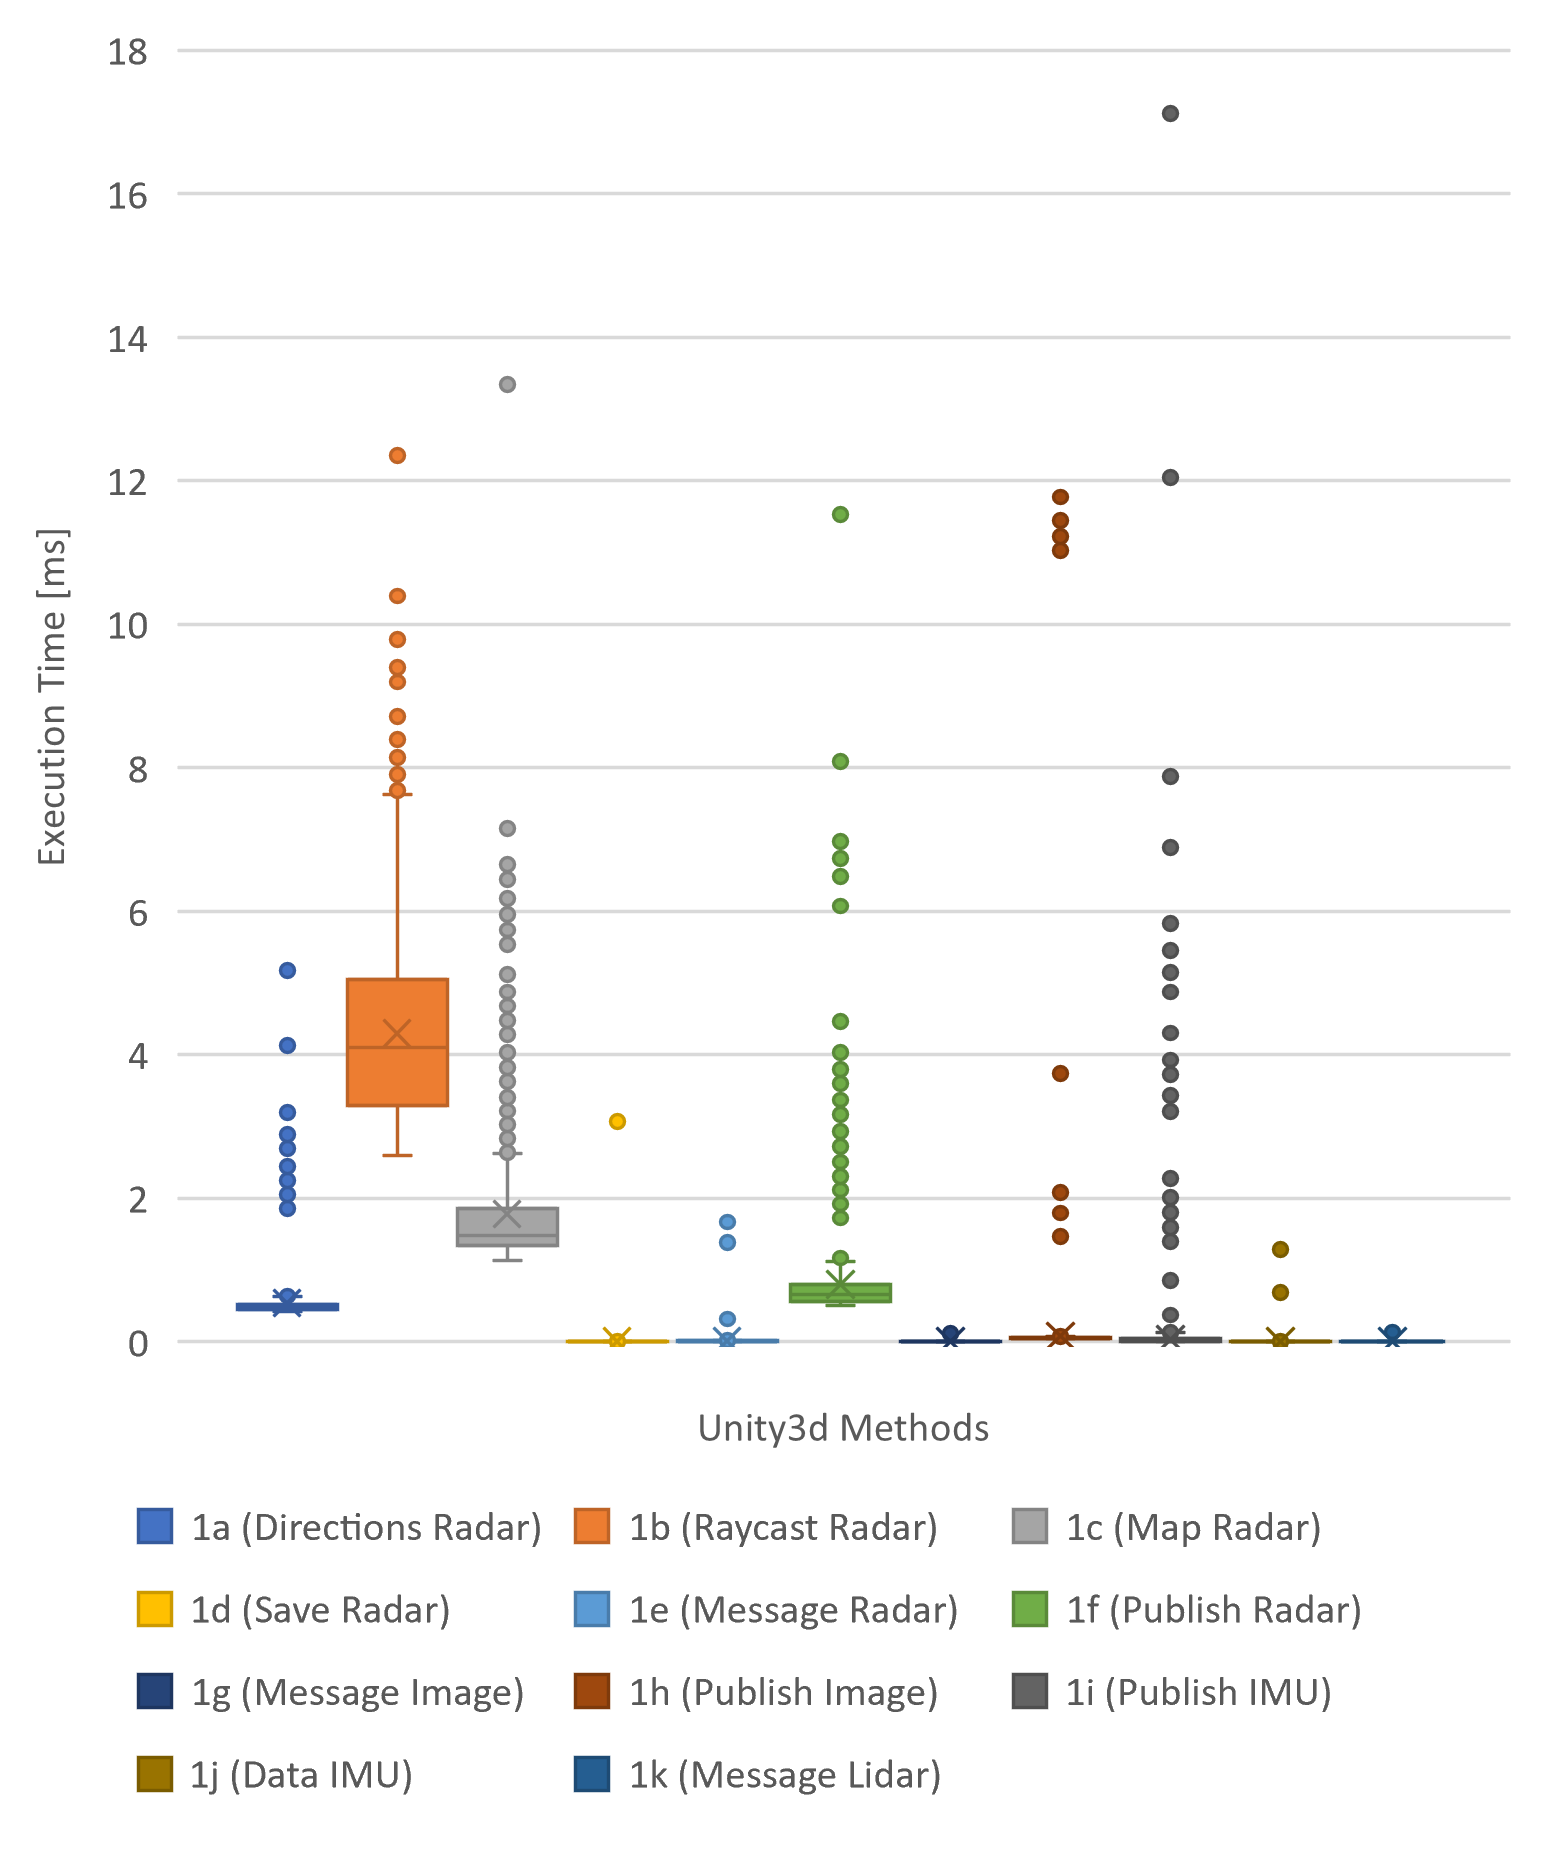
\includegraphics[height=3cm]{Bilder/Unity3d1.png}%
				\enskip
				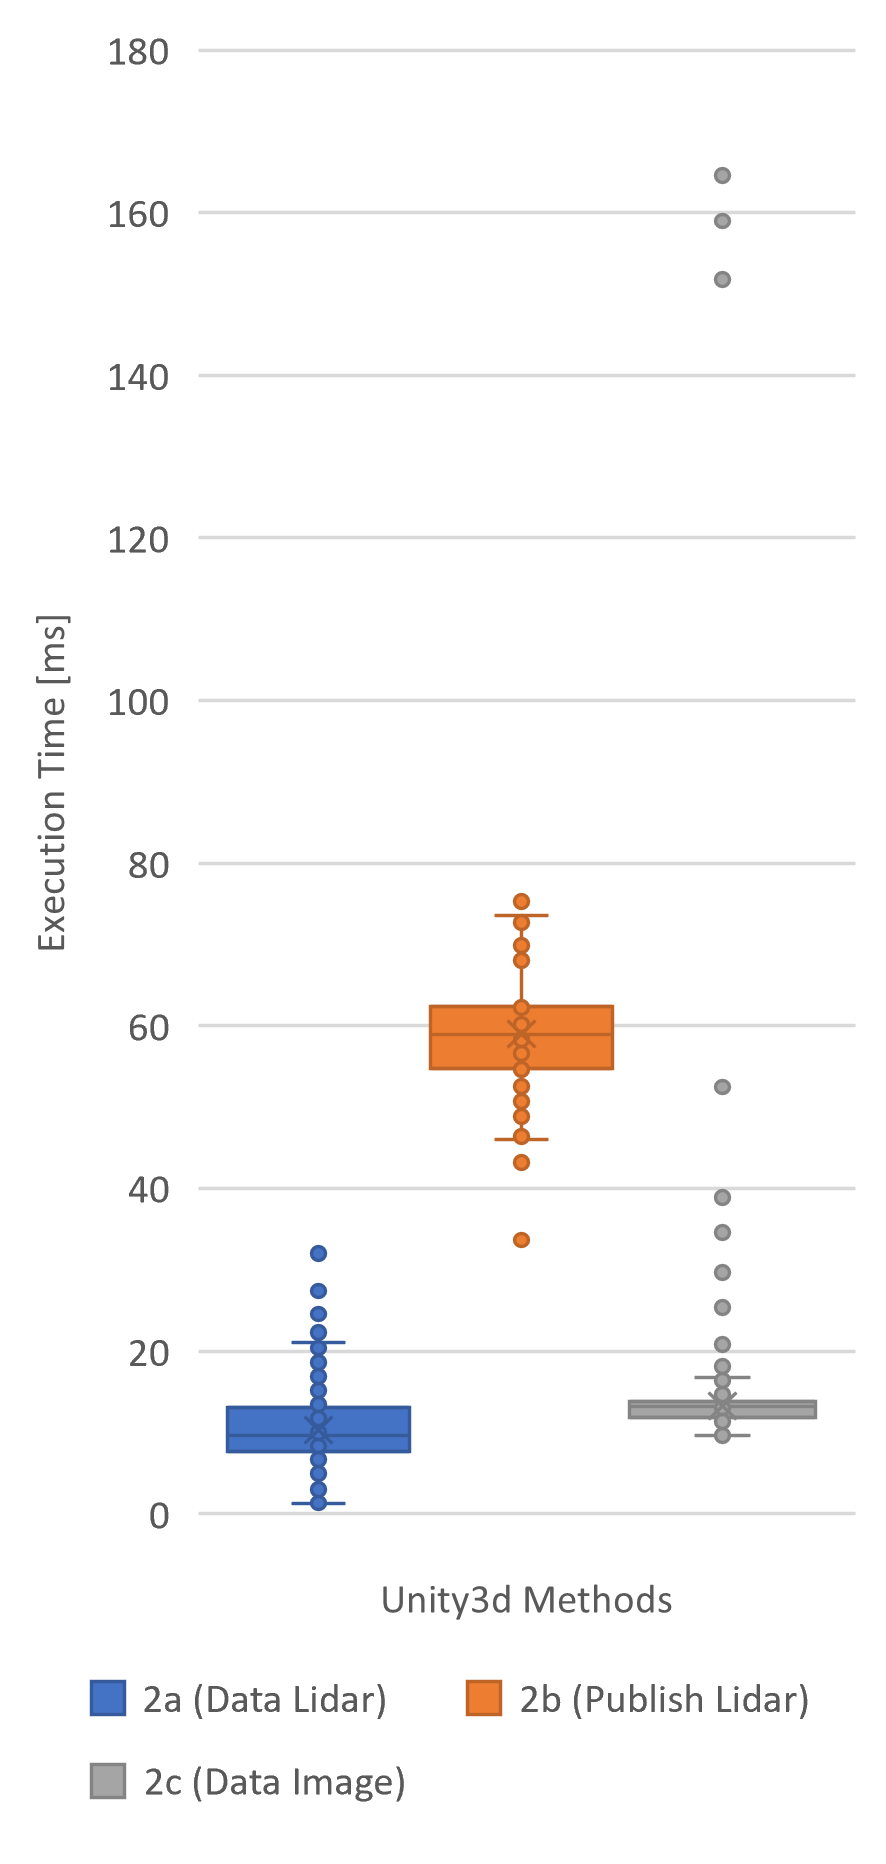
\includegraphics[height=3cm]{Bilder/Unity3d2.png}%
			}
			\caption{Unity3d methods time (total of 126000 executions)}
			\label{fig_Unity3d1}%Label für das Referenzieren 
		\end{center}
	\end{figure}
  
   For the methods that are executed in \ac{ROS2} figure \ref{fig_Ros21} provides two figures with a similar structure to figure \ref{fig_Unity3d1}. The figure to the left plots data up to 300ms and the plot to the right data up to 3s in a box and whisker representation of about 27300 executions. Again the methods that are depicted can be looked up in appendix \ref{Attachtable} in table \ref{tab_abb}. In figure \ref{fig_Ros21}, (3a) to (3h) process times at below 300ms even for exceptional outliers are shown, which is sufficient for the application at hand. Going into further detail, method (3g) that computes the bounding boxes for the \ac{LIDAR} data is noteworthy as it shows an comparable high median of just below 200ms. Thus (3g) provides a first method that can be optimized towards a lower computing time to minimize the \ac{LIDAR} data processing time.\\ 
   
    In the plot to the right it becomes clear that the execution times of (4a) to (4b) can exceed 500ms. That is a critical limit as the frequency from the data generation in Unity3d is set to two Hertz. With the methods execution time above 500ms the \ac{ROS2} network is not able to process the data in time which can lead to data being ignored. Upon further investigation, it becomes clear that these methods solely visualize data. As the data visualization is implemented with the matplotlib library for Python, finding another library more suited to plot data in a repeated cycle provides a way to improve the time needed for visualization. A further chance of improvement is given by the visualization of already processed data e.g. visualizing the bounding boxes of the \ac{LIDAR} data instead of the whole point cloud.
	\begin{figure}
		\begin{center}
			\resizebox{.9\textwidth}{!}{%
				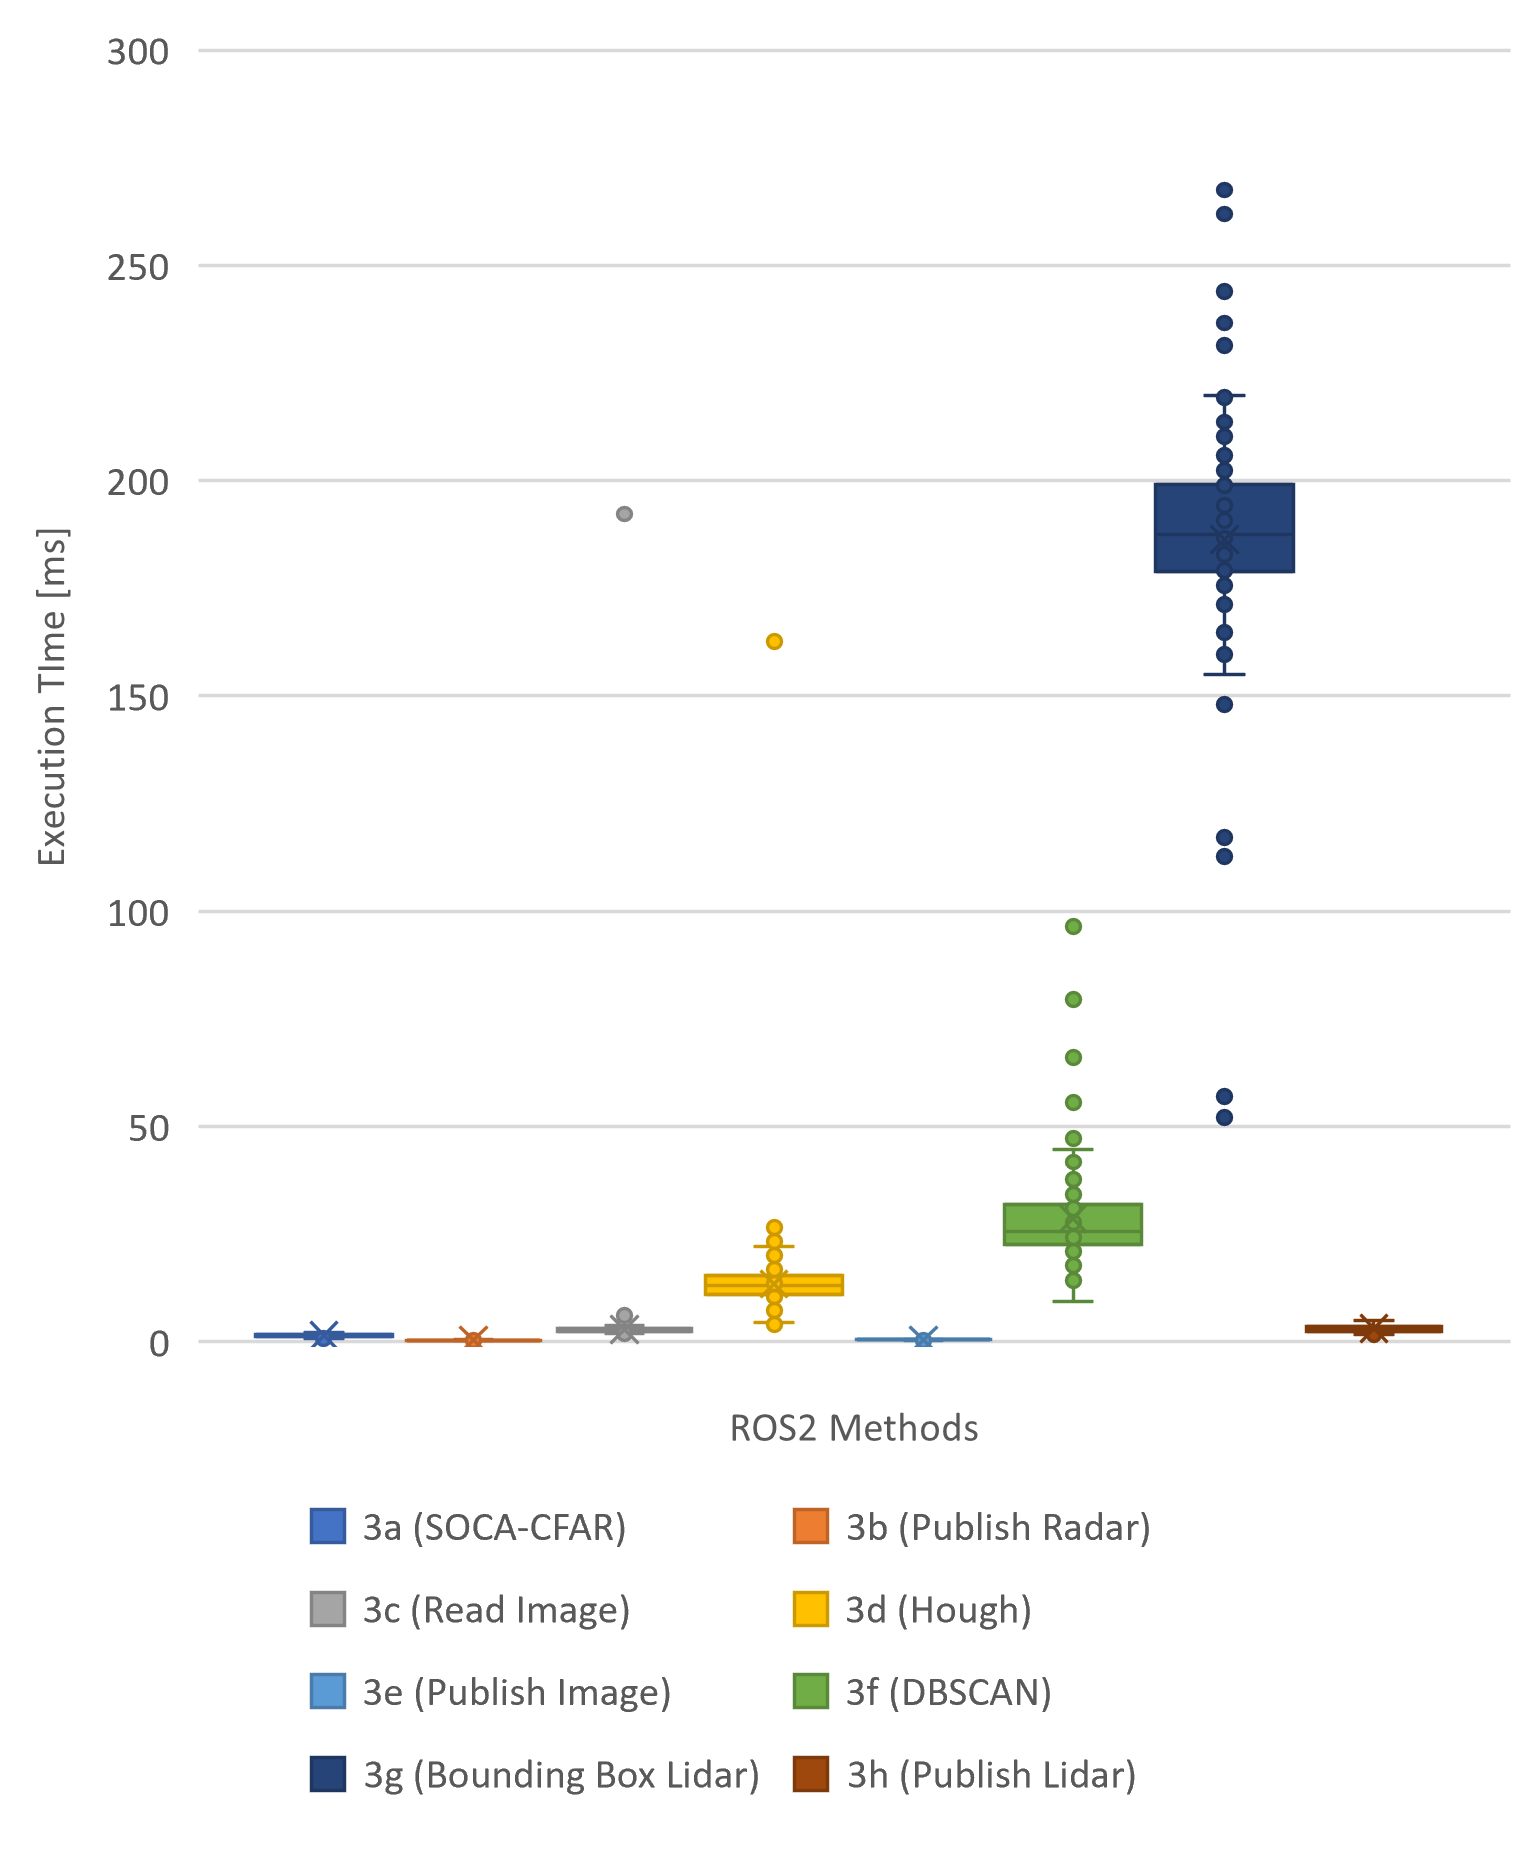
\includegraphics[height=3cm]{Bilder/ROS22.png}%
				\enskip
				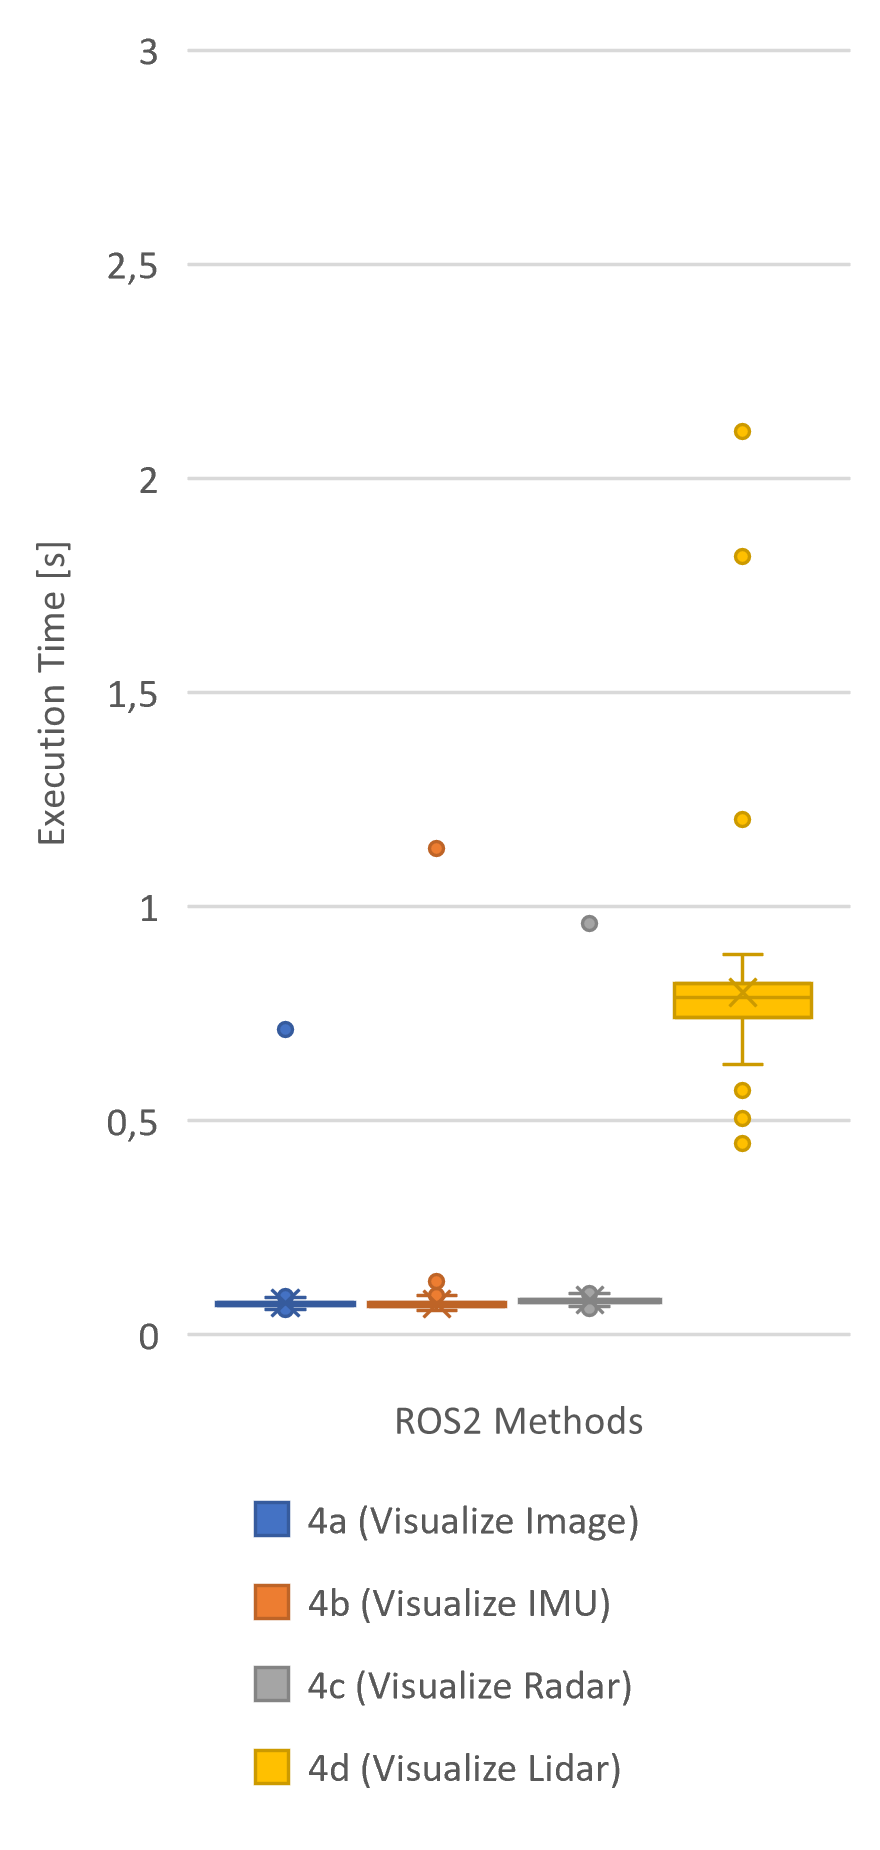
\includegraphics[height=3cm]{Bilder/ROS21.png}%
			}
			\caption{ROS2 methods time in (total of 27300 executions)}
			\label{fig_Ros21}%Label für das Referenzieren 
		\end{center}
	\end{figure}

	\section{Part Integration Test}\label{intpart}

	 Continuing with the time that is required to transmit the data, as a first step the average size of the messages that are transmitted is taken. To avoid measurements that are delayed by processing data in \ac{ROS2}, empty nodes with the only purpose of accepting data are written. In table \ref{tab_msgsize}, (5a) to (5e) show the average size of 100 message of the \ac{RADAR}, \ac{LIDAR}, \ac{IMU} and Image sensor respectively as well as the total transmitted size per second. With 285 KB/s, (5b) stands out of (5a), (5c) and (5d) and makes up a large part of the sum of messages sizes of about 291 KB/s. Considerably larger than the message size is the average intern network load of the system that is measured with the tool \textit{nload} and calculated over 100 samples. 1.62 MB/s as shown in table \ref{tab_netload} are send over the network under load of which only 24.418 KB/s are used from the operating system. The high value can be explained with the necessity of converting and resending the data between the Unity3d environment in C\# and the ROS2 environment in C++ over the Node.js framework in Java. However, a multiplication of about five relative to the total size of the messages is considered as high and can be investigated in further studies to increase the system performance and decrease the latency.\\
	 \begin{figure}[!htb]
	 	\begin{minipage}[t]{0.48\textwidth}	
	 		\begin{table}[H]	
	 			\centering
	 			\caption{Message size in ROS2}
	 			\begin{tabular}{l l } 
	 				\toprule
	 				Name  & Size  $\varnothing100$\\ 
	 				\midrule
	 				5a (Radar) & 5.78 KB/s\\
	 				5b (Lidar) & 285.37 KB/s\\
	 				5c (\ac{IMU}) & 32 B/s \\
	 				5d (Image) & 88 B/s \\\\
	 				
	 				5e Sum         & 	291.270 KB/s\\
	 				\bottomrule
	 			\end{tabular}
	 			\label{tab_msgsize}
	 		\end{table}
	 	\end{minipage}\hfill
	 	\begin{minipage}[t]{0.48\textwidth}
	 		\begin{table}[H]
	 			\centering
	 			\caption{Network Load}
	 			\begin{tabular}{l l } 
	 				\toprule
	 				Network Load & $\varnothing300s$ \\ 
	 				\midrule
	 				Idle In/Out &24.418 KB/s \\	 
	 				Publishing In/Out & 1.62 MB/s \\
	 				\bottomrule
	 			\end{tabular}
	 			\label{tab_netload}
	 		\end{table}
	 	\end{minipage}
	 \end{figure}
	 
	 Investigating the latency, to the left of figure \ref{fig_transmission}, (i) to (l) provide the values for the average transmission time from the Unity3d system to the \ac{ROS2} system. With an average of 86ms, the \ac{LIDAR} data (h) stands out from the other values but can be considered as acceptable as the \ac{LIDAR} data includes a high amount of single point values that have to be transmitted. However, more important than the average time is the reliability with which the transmission time is in a certain interval of time. Therefore, a more detailed representation of the data is shown in figure \ref{fig_transmission} to the right with a box and whiskers plot. It becomes clear that the average transmission time of the message conceal a highly scattered latency. Especially for the \ac{IMU} (5c) with only 32 B/s of data size, transmission times of above 80ms are possible with an median of below 10ms. Similar to (5c), the difference of the median to the highest latency value measured in (5b) is about 50ms. However, no requirement on the real time behaviour is set for the system and times of below 140ms are within a range that can be considered as sufficient for an adequate response in the scope of the appliance at hand. Detailing the real time definition of the appliance may be considered in further studies. 
	 
		\begin{figure}
		\begin{center}
			\resizebox{.9\textwidth}{!}{%
				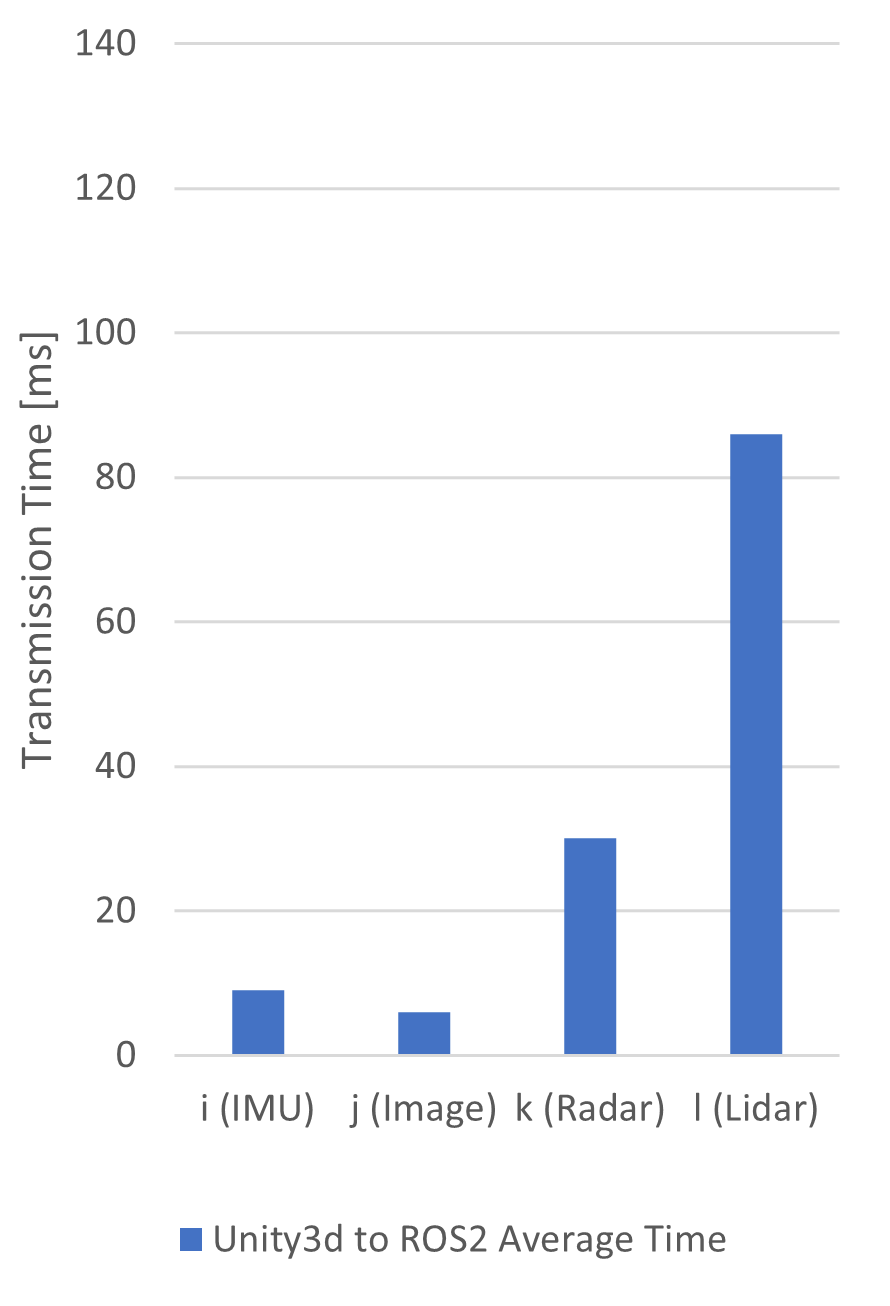
\includegraphics[height=3cm]{Bilder/TimingAver.png}%
				\enskip
				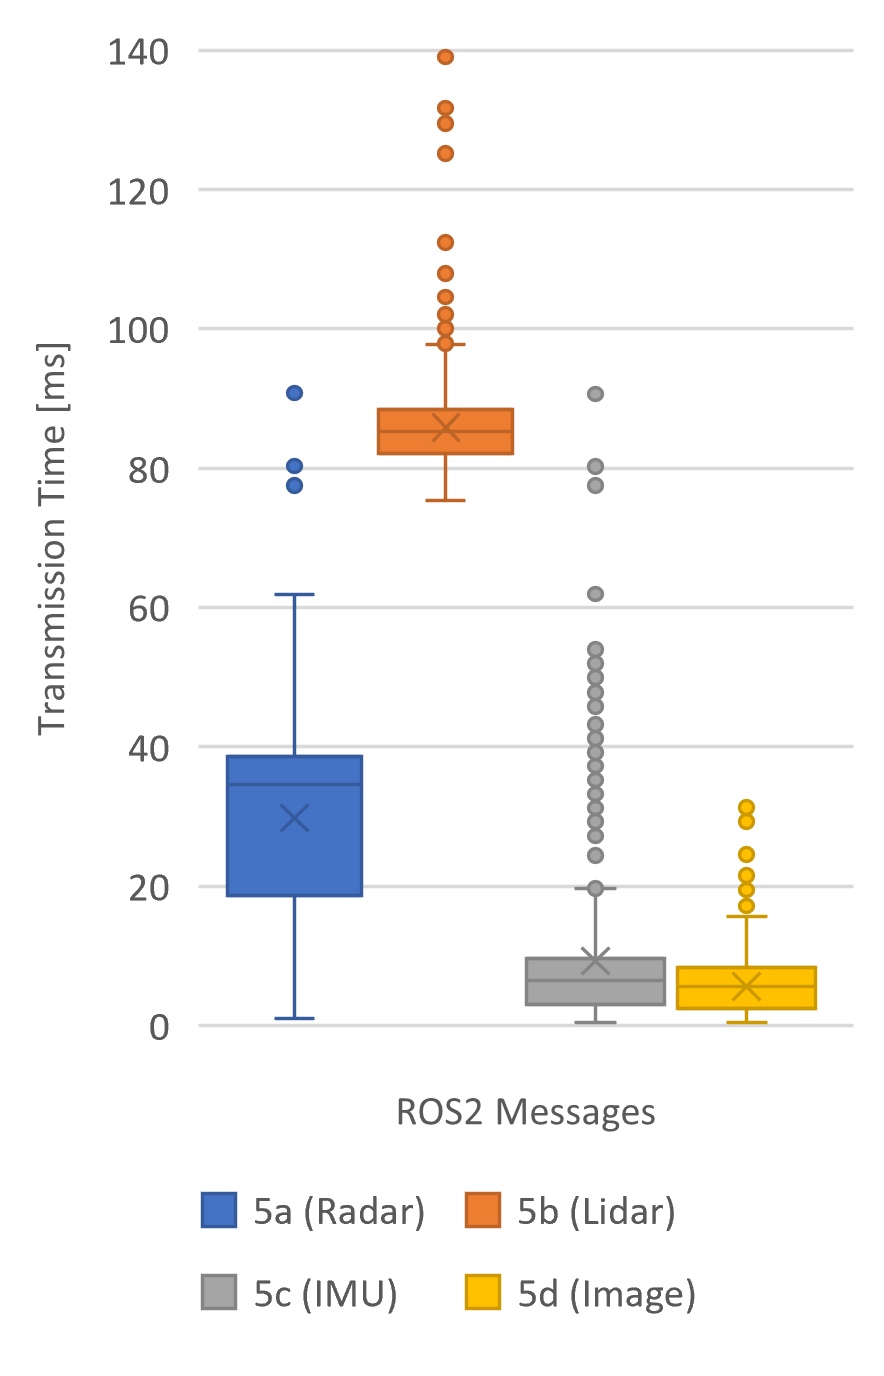
\includegraphics[height=3cm]{Bilder/Transmission.png}%
			}
			\caption{ROS2 methods time in (total of 12600 executions)}
			\label{fig_transmission}%Label für das Referenzieren 
		\end{center}
	\end{figure}
	
	\section{Validation Software} \label{validate}
	In this section, the implemented system is validated by using the proposed system architecture, the system specification and requirements defined in terms of safety. Central to the implementation is the software framework \ac{ROS2} that can be used to connect real sensors as well as virtual sensors, control actuators and share information with a control center. The library that is chosen to connect to the virtual sensors allows for a physical separation of the processing units that calculates the virtual sensors data and the subsequent processing of the data. Unity3d as the simulation environment proofed to be able to generate virtual sensor data and it is possible to resemble different types of sensors to percept the virtual environment. Therefore the chosen modules and the implemented system architecture is in compliance with the specified design. The system implementation is oriented at the V- Model and therefore complies with the demand to use a valid software safety life cycle model. Verifying the software further, the part of the regulations that relate to the design of a software framework state, that the information that result in any autonomous decision making is to be shared with the personell of the \ac{MASS} trial. The software as implemented fullfills this demand by visualizing the processed data of the sensors after each processing step.\\
	
	Continuing with a more detailed analysis, the system as implemented is tested against the criteria set in section 7.4 of \ac{VDE} 0803-3 \cite{DIN_3} and described in section \ref{Require}. A total of 14 criteria should be met in the software design and development process. In table \ref{tab_veri}, the criteria of the test that is conducted is given with the result being positive or negative. To start with the first two tests that are specified, it can be concluded that there no fault in the concept is detectable (1) and the overall system is designed with a focus on easy comprehensibility (2). With the utilization of \ac{ROS2} as a central framework, a deterministic behaviour of the data processing can be ensured (3). As only the Unity3d environment is used in the system and therefore influences of a real environment are missing, criteria (4) can not be evaluated. Both Unity3d and \ac{ROS2} provide possibilities to ad or replace components where required through the asset store in the first case and packages in the latter. This option results in a modular (5) and changeable code (6). By making use of classes and methods, the code in Unity3d is divided into several submodules that are easily testable. However, the methods of one class are dependent on each other. Therefore testing each method for itself requires a considerable amount of additional code that simulate the respective methods before the method that is to be tested. The same is the case for the code in \ac{ROS2}. With a division into nodes, classes and methods, methods are still dependent on each other. However, as the separate testing is not a requirement, criteria (7) and (8) are considered to be met. By making use of a structured process oriented at the V-model throughout every aspect of the system design is  documented which includes the intended design of the system (9), the integration test (10) that falls together with the module test (11) and the safety validation. In the module implementation, a summary is provided by every class and method that is written to ease the understanding of the purpose of the code (13). The author of the code is documented, too (14). It is noted that no liability or responsibility is taken for the code.\\
	
	

		\begin{table}[H]
		\centering	
		\caption{Safety criteria in system validation}
		\begin{tabular}{ l l } 
	\toprule
	Criteria & Criteria met \\
	\midrule
	(1)  Without faults in the concept  &  \cmark \\
	(2)  Easily comprehensible 			&   \cmark\\
	(3)  Display a deterministic behaviour &\cmark\\
	(4)  Fault tolerant in the event of external events &\xmark$^1$\\
	(5)  Modularity 					&\cmark\\
	(6)  Changeable code 				&\cmark\\
	(7)  Divided into several more detailed submodules &\cmark $^2$\\
	(8)	 Testable 						&\cmark\\
	(9)  Intended design of the system documented &\cmark\\
	(10) Integration Test documented	&\cmark\\
	(11) Module test documented 		&\cmark\\
	(12) Safety validation of the system is documented &\cmark\\
	(13) Software is documented &\cmark\\
	(14) Responsibility is documented  &\cmark $^3$\\
	\bottomrule
	
	\multicolumn{2}{l}{\small $^1$ no test specified, only the simulation is used as a test environment } \\
	\multicolumn{2}{l}{\small $^2$ submodules are dependent on each other, separate testing requires more effort } \\
	\multicolumn{2}{l}{\small $^3$ translates to the documentation of the author of the code} \\
\end{tabular}
\label{tab_veri}
\end{table}


  
\chapter{Conclusion and Outlook}\label{ConFut}
 	\section{Conclusion} \label{Con}
    
    In this thesis a software architecture for virtual sensors in autonomous small vessels is conceptualized and implemented that allows for the integration of virtual and physical sensors.  A structured and safe design process is obtained by following the V-model for software designs. To avoid possible restrictions imposed by the limitations of the chosen software frameworks, a focus is laid on the system specification. With \ac{ROS2}, Unity3d and Node.js a solution is specified which not only meets the requirements but opens up the opportunity for further implementations that expand the scope of the introduced system. In conjunction with the system design, an Unity3d scene is created that resembles the topographic as well as visual data from an existing location. Furthermore, a viable way is shown to reconstruct and implement a \ac{RADAR} in a virtual environment. By integrating four different virtual sensors into the scene, the scalability of the design is demonstrated. It is shown, that algorithms in \ac{ROS2} which comprise a cluster analysis (\ac{DBSCAN}) and a false alarm detector (\ac{SOCA-CFAR}) are able to process the environmental data of the sensors and thus functions are implemented that are vital for the navigation subsystem of a \ac{GNC} system. Furthermore, routines that calculate bounding boxes around clustered \ac{LIDAR} data provides condensed environmental data and a way is shown to connect to the guidance subsystem of a \ac{GNC} system with a low data rate.\\
    
    In compliance with the defined requirements, the final result of this thesis is an architecture that allows for the easy incorporation of software that is vital to the design of autonomous inland navigation vessels. In addition, a variety of tested algorithms demonstrate the diverse opportunities that result of the chosen solution.
    
 	\section{Suggestions for Future Work} \label{Sug}
	Further waypoints of detailing the proposed architecture are to be found in the specified functions of a \ac{GNC} system. Starting with the implementation of a guidance subsystem that utilizes the information of the guidance subsystem, also a control subsystem has to be realized that connects to the actors of a vessel. It remains open which algorithms prove to full fill the required functionality of this subsystems. In this context, modelling the virtual scene in greater detail is clearly beneficial to the quality of information that can be derived from the simulation and exported to the behaviour of a real vessel. Especially adding a more sophisticated simulation of water is expected to increase the possibilities of testing algorithms closer to conditions that may occur in a real world scenario.  With the architecture providing an easy way to embed real sensors, it remains open how the system reacts to a substitution of the virtual sensors and influences of a real environment.\\
	
	 With the focus on demonstrating the versatility of the architecture, the focus in the implementation is on a variety of use cases instead of optimizations. Therefore, concerning the realized software, a number of possible improvements show up e.g. improving the GPU utilization in Unity3d. The interested reader may refer to appendix \ref{Attachlistb} where possible improvements to the existing software are detailed.

  \printbibliography % Anzeigen der Bibliography	 
 
  \clearpage
  \listoffigures
  
  \clearpage
  \listoftables
  
  \clearpage
  %\lstlistoflistings
  \appendix		
  \chapter{Execution time of the systems methods}\label{Attachtable}
 Table \ref{tab_abb} details the execution time on average of every method that is used in this thesis. In the first column, an abbreviation for the method is defined. Followed by the class the method can be found in, the methods name is given. The name is followed by the average execution time of the according message. The last column shows the average execution time of all methods of one class. Methods (1) to (2) belong to the Unity3d environment and methods (3) to (4) relate to the \ac{ROS} system. Every horizontal single line represents a different sensor and every horizontal double line indicates a different system. An exception from the previous explanation is made for the case (5a) to (5d). These are the messages for a \ac{ROS} interface and the average execution time translates to the time that is needed for a transmission from Unity3d to \ac{ROS}. As the messages are transmitted in parallel to each other, they are not summed up. 
 \newpage
	\begin{table}[H]
	\centering
	\caption{Average execution time of methods}
	\begin{tabular}{l l l c c }  
		Abbreviation&Class/Package& Method/Message&\multicolumn{1}{p{1cm}}{$\varnothing$\newline [ms]} &\multicolumn{1}{p{1cm}}{ Sum\newline [ms]} \\ 
		\midrule\midrule
		1a (Directions Radar)	& RadarSensor &Calculate direc.()&1&\multirow{6}{*}{6}\\
		1b (Raycast Radar)	& RadarSensor 	& CommandRaycast	&4&	\\
		1c (Map Radar)		& RadarSensor 	& MapToPlane() 		&2&	\\
		1d (Save Radar)	& RadarSensor 	& Save() 			&0&	\\
		1e (Message Radar)	& ROSPublishRadar1 & SetMessage()	&0&	\\ 	
		1f (Publish Radar)	& ROSPublishRadar1 & Publish() 		&1&	\\
		\midrule
		2c (Data Image)	& SensorImage 	& UpdateImage()		&13&\multirow{3}{*}{13}	\\
		1g (Message Image)	& ROSPublishImg & SetMessage() 		&0&	\\
		1h (Publish Image)	& ROSPublishImg	& Publish()			&0&	\\
		\midrule
		1i (Publish IMU)	& ROSPublishIMU	& Publish() 		&0&\multirow{2}{*}{0}	\\	
		1j (Data IMU)		& SensorIMU		& GetIMUData()		&0&	\\
		\midrule
		1k (Message Lidar)	& ROSPublishXYZ	& SetMessage 		&0&\multirow{3}{*}{69}	\\				
		2a (Data Lidar)	& LidarSensor	& Lidar() 			&10&	\\
		2b (Publish Lidar)	& ROSPublishXYZ	& Publish() 		&59&	\\	
		\midrule\midrule
		5a (Radar) 	&gnc/interfaces&/radar1/img 								&30&30	\\	
		5b (Lidar) 	&gnc/interfaces&/lidar1/xyz								&86&86	\\
		5c (IMU) 	&gnc/interfaces&/imu1/accvel								&9&9	\\
		5d (Image) 	&gnc/interfaces&/cam1/pixel								&6&6	\\
		\midrule\midrule
		3a (SOCA-CFAR)         & get\_radar &bounding\_box() 	&2&	\multirow{3}{*}{83}\\
		3b (Publish Radar)   & get\_radar &publish()			&0&	\\	
		4c (Visualize Radar) & get\_radar &visualize\_cluster()&81&	\\
		\midrule
		3c (Read Image)      & get\_image & read\_image()		&3&\multirow{4}{*}{91}	\\	
		3d (Hough)             & get\_image & lines\_extraction()&13&	\\
		3e (Publish Image)   & get\_image & publish\_lines() 	&1&	\\
		4a (Visualize Image) & get\_image & visualization()	&74&	\\
		\midrule	
		3f (DBSCAN)            & get\_lidar & dbscan()			&29& \multirow{4}{*}{1017}	\\
		3g (B. Box Lidar)& get\_lidar & bounding\_box()	&186&	\\
		3h (Publish Lidar)   & get\_lidar & publish()			&3&	\\
		4d (Visualize Lidar) & get\_lidar & visualize\_cluster()&799&	\\
		\midrule
		4b (Visualize IMU)   & get\_imu   & visualize\_data()	&72& \multirow{1}{*}{72}	\\	
		% Change position, group with other image times

	
		
	\end{tabular}
	\label{tab_abb}
\end{table}
\chapter{Improvements to the existing system}\label{Attachlistb}	
In the following, a list of implementations is shown that may improve the software of the system. In itself the single points are expected to contribute only little to the overall system performance but may increase the performance considerably when summed up.
\begin{itemize}
	\item The \ac{GPU} utilization in the Unity3d scene is low even with a low framerate due to a high computational effort. Parallelizing more tasks would contribute to a higher framerate as the computation load is focused not only on one \ac{GPU} unit. 
	\item The intern network load of the operating system is considerably higher than the messages that are send from Unity3d. The image message as implemented in this work provides an example of dividing a message in metadata that is send over the \ac{ROS} network and data that is saved by the operating system and captured by \ac{ROS} upon request. However it has to be kept in mind that this approach is not in compliance with the design rules for a \ac{ROS} package.
	\item As shown, visualizing high amounts of data with the python library \textit{matplotlib} takes a long time when executed in the \ac{ROS} environment. Finding another way to plot data with \textit{matplotlib} or find an optimized library for this purpose may prove to be advantageous.   
	\item The calculation of the bounding boxes of the \ac{LIDAR} cluster takes a long time due to recurrent iterations over the dataset. Elaborate on the used algorithm can result in lower computation time. 
	\item Due to the raycasts in the simulation that reconstruct the \ac{LIDAR} laser beams, the resulting virtual sensor takes a long time until all rays are send. Dividing the raycast into beams that are independent from each other could provide an opportunity to utilize multiple cores in addition to the \textit{JobHandle} that is already used. Investigating in other steps that need a long time to be executed may result in further possibilities of optimization.
	\item  As the methods used in this work are dependent on each other, they were not tested in an isolated environment. Creating data that simulates the output of methods, single routines can be tested and influences, e.g. queing data, of other methods can be avoided.
	\item The rendering of the reflection on water requires a separate camera in the Unity3s scene. Several water planes are used and thus the computational effort is rising. Avoiding a multitude of rendered cameras can increase the frames per second with which events are calculated in Unity3d. As proposed, using a more elaborated water simulation can solve this problem.
	\item To simulate the analogous beam signal of a real \ac{RADAR}, many ray casts are necessary in Unity3d. Using a box raycast that is given by the physics engine of Unity3d, instead of many rays, one cast over an area is made with a three dimensional shape. The advantage is the reduced computational effort due to the reduced ray casts.
	\item Instead of using a decentralised solution in which every data is saved locally in the classes that transmit data to other classes, a central location to can be allocated from where the classes do queries for the data they need. This avoids the recurrent allocation of memory for the data e.g. from sensors.
	
\end{itemize}
  
  \clearpage
\end{document}
